\documentclass[11pt]{article}
\usepackage[margin=1in]{geometry}
\usepackage{amsmath,amssymb,amsthm}
\usepackage{booktabs}
\usepackage{enumitem}
\usepackage{xcolor}
\usepackage[colorlinks=true,linkcolor=blue!50!black,urlcolor=blue!50!black,citecolor=blue!50!black]{hyperref}
\usepackage{microtype}
\usepackage{tikz}
\usetikzlibrary{calc}
\usepackage{pdflscape}
\usepackage{graphicx}
\usepackage{longtable}
% shared TikZ macros for the geometry figures (unit cells; source cell at the origin, target cell at the offset)
\newcommand{\cube}[3]{%
 \draw[gray!55,thin] (#1,#2,#3) -- ++(1,0,0) -- ++(0,1,0) -- ++(-1,0,0) -- cycle;
 \draw[gray!55,thin] (#1,#2,#3+1) -- ++(1,0,0) -- ++(0,1,0) -- ++(-1,0,0) -- cycle;
 \draw[gray!55,thin] (#1,#2,#3) -- ++(0,0,1) (#1+1,#2,#3) -- ++(0,0,1) (#1+1,#2+1,#3) -- ++(0,0,1) (#1,#2+1,#3) -- ++(0,0,1);}
\newcommand{\facex}[4]{\fill[#4,opacity=0.40] (#1,#2,#3) -- ++(0,1,0) -- ++(0,0,1) -- ++(0,-1,0) -- cycle; \draw[#4,thick] (#1,#2,#3) -- ++(0,1,0) -- ++(0,0,1) -- ++(0,-1,0) -- cycle;}
\newcommand{\facey}[4]{\fill[#4,opacity=0.40] (#2,#1,#3) -- ++(1,0,0) -- ++(0,0,1) -- ++(-1,0,0) -- cycle; \draw[#4,thick] (#2,#1,#3) -- ++(1,0,0) -- ++(0,0,1) -- ++(-1,0,0) -- cycle;}
\newcommand{\facez}[4]{\fill[#4,opacity=0.40] (#2,#3,#1) -- ++(1,0,0) -- ++(0,1,0) -- ++(-1,0,0) -- cycle; \draw[#4,thick] (#2,#3,#1) -- ++(1,0,0) -- ++(0,1,0) -- ++(-1,0,0) -- cycle;}
\newcommand{\axes}{\draw[->,gray] (-0.3,-0.3,0) -- ++(0.5,0,0) node[right,gray,font=\tiny]{$x$}; \draw[->,gray] (-0.3,-0.3,0) -- ++(0,0.5,0) node[above right,gray,font=\tiny]{$y$}; \draw[->,gray] (-0.3,-0.3,0) -- ++(0,0,0.5) node[above,gray,font=\tiny]{$z$};}
\tikzset{geo/.style={x={(0.95cm,-0.28cm)}, y={(0.62cm,0.42cm)}, z={(0cm,0.95cm)}, scale=1.0, every node/.style={font=\footnotesize}}}

% one tikzpicture per sub-geometry, drawn with the macros of figs.tex.
% Source cell at the origin (red = source face F'), target cell displaced by
% Delta (blue = target face F). Same coordinates as figcontact/figshell/figextra.
\newcommand{\gbox}[1]{\begin{tikzpicture}[geo]\useasboundingbox (-0.7,-0.7,-0.3) rectangle (2.7,2.4,2.5); #1\end{tikzpicture}}

\newcommand{\figSS}{\gbox{\cube{0}{0}{0}\cube{1}{0}{0} \facex{1}{0}{0}{red} \facex{1}{0}{0}{blue} \axes}}
\newcommand{\figEf}{\gbox{\cube{0}{0}{0}\cube{1}{0}{0} \facey{0}{0}{0}{red} \facey{0}{1}{0}{blue}}}
\newcommand{\figEc}{\gbox{\cube{0}{0}{0} \facez{0}{0}{0}{red} \facey{0}{0}{0}{blue}}}
\newcommand{\figEcx}{\gbox{\cube{0}{0}{0}\cube{1}{1}{0} \facex{1}{1}{0}{blue} \facey{1}{0}{0}{red}}}
\newcommand{\figVc}{\gbox{\cube{0}{0}{0}\cube{1}{1}{0} \facez{0}{0}{0}{red} \facez{0}{1}{1}{blue}}}
\newcommand{\figVp}{\gbox{\cube{0}{0}{0}\cube{1}{1}{1} \facez{1}{0}{0}{red} \facex{1}{1}{1}{blue}}}
\newcommand{\figPa}{\gbox{\cube{0}{0}{0} \facex{0}{0}{0}{red} \facex{1}{0}{0}{blue} \axes}}
\newcommand{\figPb}{\gbox{\cube{0}{0}{0}\cube{1}{0}{0} \facex{0}{0}{0}{red} \facex{2}{0}{0}{blue}}}
\newcommand{\figPas}{\gbox{\cube{0}{0}{0}\cube{1}{0}{0} \facey{1}{0}{0}{red} \facey{0}{1}{0}{blue}}}
\newcommand{\figPbs}{\gbox{\cube{0}{0}{0}\cube{1}{1}{0} \facex{0}{0}{0}{red} \facex{2}{1}{0}{blue}}}
\newcommand{\figXg}{\gbox{\cube{0}{0}{0}\cube{1}{0}{0} \facex{0}{0}{0}{red} \facey{0}{1}{0}{blue}}}
\newcommand{\figXgb}{\gbox{\cube{0}{0}{0}\cube{1}{1}{0} \facez{0}{0}{0}{red} \facex{2}{1}{0}{blue}}}
\newcommand{\figXgc}{\gbox{\cube{0}{0}{0}\cube{1}{1}{0} \facey{0}{0}{0}{red} \facex{2}{1}{0}{blue}}}
\newcommand{\figXgd}{\gbox{\cube{0}{0}{0}\cube{1}{1}{1} \facey{0}{0}{0}{red} \facex{2}{1}{1}{blue}}}
\newcommand{\figPasb}{\gbox{\cube{0}{0}{0}\cube{1}{1}{0} \facez{1}{0}{0}{red} \facez{0}{1}{1}{blue}}}
\newcommand{\figPbsb}{\gbox{\cube{0}{0}{0}\cube{1}{1}{1} \facex{0}{0}{0}{red} \facex{2}{1}{1}{blue}}}


\newtheorem{theorem}{Theorem}[section]
\newtheorem{proposition}[theorem]{Proposition}
\newtheorem{lemma}[theorem]{Lemma}
\newtheorem{corollary}[theorem]{Corollary}
\theoremstyle{remark}
\newtheorem{remark}[theorem]{Remark}

\newcommand{\dd}{\mathrm{d}}
\newcommand{\ii}{\mathrm{i}}
\newcommand{\asinh}{\operatorname{asinh}}
\newcommand{\atan}{\operatorname{atan}}
\newcommand{\Rr}{\mathbb{R}}
\newcommand{\code}[1]{\texttt{#1}}
\newcommand{\Gs}{G_{\mathrm{s}}}
\newcommand{\geofig}[2]{\begin{center}#1\\[2pt]{\footnotesize #2}\end{center}}

\allowdisplaybreaks
\setlength{\emergencystretch}{3em}

\title{The Moments of Gila:\\ Closed Forms for Every Panel-Pair Integral of $r^{m}$}
\author{Claude (Anthropic, Claude Fable 5.1)\\[2pt]\small prepared for Paul Virally, GilaElectromagnetics}
\date{6 September 2026}

\begin{document}
\maketitle

\begin{abstract}
The companion document \emph{The Integrals of Gila} proved that every moment
$I_m(F,F') = \int_F\int_{F'}|\mathbf{x}-\mathbf{y}|^m\,\dd S'\,\dd S$ of a pair of
axis-aligned rectangles is an elementary function of the edge lengths, and left the
formulas themselves to be found. This document finds them. Every face pair of two
touching cuboid cells on a regular lattice falls into ten Table-1 codes, which resolve
into fifteen inequivalent sub-geometries once the offsets of the convolution weights are
distinguished; for all fifteen, and for every integer $m\ge -1$, we give closed forms and
verified recurrences with explicit elementary seeds, together with a floating-point
arrangement whose \code{Float64} evaluation loses at most $0.91$ decimal digits against a
$320$-bit reference over aspect ratios from $10^{-6}$ to $10^{6}$ and $m = -1,\ldots,12$.
Correctness is at the reference evaluator's own convergence floor, $10^{-44}$ to
$10^{-68}$ relative, at eleven cell shapes and at all $144$ face pairs of the four
touching-cell offsets. The series built from these moments reproduces Gila's
\code{wekS}, \code{wekE}, \code{wekV} at \code{intOrd} $48$ and $64$ and its order-9 fixed
rule for the non-touching pairs to the accuracy of those numerics, and exposes a defect in
the order-9 rule on slender cells. Four independent derivation families --- polar
coordinates with the secant-power reduction, the divergence recursion on the product box,
the box-potential route, and numerical discovery with exact coefficient recovery --- were
run without knowledge of each other and converged on the same five primitive blocks;
that convergence, and not any single derivation, is the reason to believe the result. The
deliverable is \code{notes/moments/moments.jl}, a standalone Julia file generic in the
number type, with \code{verify.jl} and \code{gilacmp.jl} producing every table quoted here.
\end{abstract}

\tableofcontents

\section{Overview}
\label{sec:over}

\subsection{What was asked}

The task statement in \code{notes/PROMPT\_integrals.md} was: for each of the ten
rectangle-pair geometries that occur between touching cells on a regular grid, produce
elementary closed forms for $I_{-1}$ and for every odd moment $I_{2m+1}$, either as an
explicit formula valid for general $m$ or as a verified recurrence in $m$ with explicit
elementary seeds, together with a cancellation-free floating-point arrangement of each;
verify each against an independent high-precision reference to at least $10^{-30}$
relative for $m = -1,\ldots,12$ at cubic cells, at slender cells with aspect ratios
$10^{-3}$ and $10^{3}$ in each direction and at the two cell shapes Gila actually uses;
measure a digits-lost table over aspect ratios $10^{-6}$ to $10^{6}$ and keep the loss
under one decimal digit; demonstrate that the resulting power series reproduces Gila's
\code{wekS}, \code{wekE}, \code{wekV} and its order-9 fixed-rule values; and ship a
standalone Julia implementation generic over the number type.

The ten codes, in the notation of Table~1 of \emph{The Integrals of Gila}, are S
(coincident faces), Ef (coplanar, sharing an edge), Ec (perpendicular, sharing an edge),
Vc (coplanar, sharing only a corner), Vp (perpendicular, sharing only a corner), P1 and P2
(parallel, one or two cell lengths apart, aligned), P1s and P2s (the same, laterally
shifted by one cell length), and Xg (perpendicular planes whose faces do not meet). Of
these, S was already solved for every $m$; $I_{-1}$ was known for Ef and Ec; nothing was
known for the rest.

\subsection{The result}

All ten Table-1 codes are done, and they are more than ten geometries. Classifying the
$144$ face pairs $(\Delta, F, F')$ of the four touching-cell offsets by the exact per-axis
convolution signature (Section~\ref{sec:cat}) splits Xg into four inequivalent
sub-geometries, and P1s and P2s into two each, giving \textbf{fifteen} sub-codes:
S, Ef, Ec, Vc, Vp, P1, P2, P1s, P1s-b, P2s, P2s-b, Xg, Xg-b, Xg-c, Xg-d, with the counts
$7, 6, 34, 5, 22, 8, 1, 8, 8, 2, 3, 12, 20, 2, 6$ summing to $144$. For all fifteen and
for every integer $m \ge -1$ there is now a closed form: an explicit elementary expression
where one is useful, and always a finite ladder of exact two-term recurrences in $m$ whose
seeds at $m = -1$ and $m = 0$ are the elementary functions $\asinh$, $\atan$ and square
roots of sums of squares. Against the $320$-bit reference evaluator \code{pairMom} the
worst relative error over the fifteen sub-codes, the eleven prescribed cell shapes and
$m = -1,\ldots,12$ is $7.35\times10^{-44}$, with zero of $2310$ values above the
$10^{-30}$ bar, and over all $144$ face pairs at $m = -1,\ldots,8$ it is
$1.91\times10^{-48}$ with zero of $1440$ above the bar; in both cases the residual is the
reference's own quadrature refinement residual, not the formulas', which order refinement
demonstrates by falling $8$ to $14$ orders per order-step with no floor. The
cancellation-free arrangement loses at most $\mathbf{0.91}$ decimal digits in
\code{Float64} over the $13\times 14$ aspect grid $a/b, c/b \in [10^{-6},10^{6}]$ and
$m = -1,\ldots,12$, with zero cells above one digit out of roughly $37\,000$ measured. The
series assembled from these moments reproduces \code{wekS}, \code{wekE}, \code{wekV} to
$6.3\times10^{-11}$ (S), $2.9\times10^{-10}$ (Ef), $9.3\times10^{-11}$ (Ec),
$5.0\times10^{-10}$ (Vc) and $1.8\times10^{-9}$ (Vp) at \code{intOrd} $48$, with the
order-$64$ values lying between the order-$48$ values and the series, and reproduces the
order-9 fixed rule for the non-touching pairs to $10^{-16}$--$10^{-13}$ on cubic cells.

\subsection{How to use it}
\label{sec:use}

The deliverable is \code{notes/moments/moments.jl}: $1720$ lines, no package
dependencies, generic in the number type (\code{BigFloat} in gives \code{BigFloat} out;
\code{Float32} works; \code{Rational} panels give exactly the values of the corresponding
float panels). A panel is a triple of coordinate intervals with one axis degenerate,
\code{((x1,x2),(y1,y2),(z1,z2))}. The three entry points are

\begin{center}\small
\begin{tabular}{@{}ll@{}}
\toprule
call & returns \\
\midrule
\code{pairMoments(A, B, mMax; tol = nothing)} & \code{Vector} with \code{out[m+2]} $= I_m$, $m = -1,\ldots,\code{mMax}$ \\
\code{faceMoments(D, F, Fp, s, mMax; tol = nothing)} & the same for face $F$ of a cell at offset \code{D} against $F'$ \\
\code{momentSeries(A, B, f, mMax)} & \code{(value, rel)}: $\int_A\int_B g$ and $|\text{last term}|/|\text{sum}|$ \\
\bottomrule
\end{tabular}
\end{center}

\noindent
Even $m$ is returned as well as odd; it costs nothing, since the same ladder carries both
parities. \code{tol} defaults to \code{nothing}, which makes the box breakpoints exactly
rational; passing a number instead merges breakpoints closer than \code{tol} relative to
the axis extent, which is the right choice when the panel coordinates are not exactly
representable (Section~\ref{sec:sliver}). \code{momentSeries} sums
$\frac{1}{4\pi f^2}\sum_n \frac{(2\pi\ii f)^n}{n!} I_{n-1}$ and returns its own
convergence indicator; that indicator is an honest upper bound on the truncation error in
all $240$ rows of the audit's series sweep, over-stating by a factor between $3.4$ and
more than $10^{3}$ and never under-stating. \code{mMax}$\,=12$ is a $\lambda/8$ tool: at a
$\lambda/4$ cell it leaves up to $7.5\times10^{-3}$ relative error on the far sub-codes,
and \code{mMax}$\,=30$ removes that.

The file also carries the plain explicit closed forms of Sections~\ref{sec:cop} and
\ref{sec:prp} (\code{momSlf}, \code{momFlt}, \code{momVtxCop}, \code{momPar},
\code{prpMom}, \code{vcMom}, \code{vpMom}, \code{xgMom}). They are cross-checks only: they
are correct but are \emph{not} arranged against cancellation, and lose up to $22.6$ digits
in \code{Float64}. Every actual evaluation should go through \code{pairMoments}.

Verification is reproduced by
\begin{center}\small
\code{JULIA\_NUM\_THREADS=1 julia -{}-startup-file=no verify.jl a|b|c|d|e}
\end{center}
which writes \code{tables/\{a,b,c,d,e\}\_*.txt}: (a) correctness at the eleven shapes,
(b) all $144$ face pairs against \code{pairMom}, (c) cross-checks against the explicit
forms plus homogeneity, symmetries, orientation invariance and the \code{tol} test,
(d) the digits-lost grids, (e) timing. The whole run is $7$ minutes $5$ seconds
single-threaded; only part (b) calls \code{pairMom} and only part (c) calls
\code{pairKer}. Part (a) reads \code{refcache.txt}, a $1155$-line cache of $320$-bit
\code{pairMom} values that took $36.7$ minutes to build, so no cached case is recomputed.

The comparison with Gila's own numerics is
\begin{center}\small
\code{JULIA\_NUM\_THREADS=1 julia -{}-startup-file=no -{}-project=<env> gilacmp.jl a|b|c}
\end{center}
with \code{<env>} any environment in which \code{using GilaElectromagnetics} works. It
writes \code{tables/f\_gila\_\{a,b,c\}.txt}: (a) \code{wekS}/\code{wekE}/\code{wekV} at
\code{intOrd} $48$ and $64$ against the series, (b) the order-9 fixed rule on every
non-touching face pair, (c) the frequency homogeneity of the series terms. Part (a) takes
$37$ minutes, $36$ of them inside Gila's own weak integrals; part (b) $35$ minutes, nearly
all of it in $280$ \code{BigFloat} series sums; part (c) $5$ seconds.

\subsection{How to read this document}

Section~\ref{sec:struct} is the part worth reading first: it sets out the single
decomposition that all fifteen geometries share, the five primitive blocks it terminates
in, and the fact that four independent derivation families found the same blocks.
Sections~\ref{sec:cop} and \ref{sec:prp} then treat the coplanar/parallel and the
perpendicular families, one subsection per sub-code, each with its figure, its derivation,
its boxed formula or recurrence with seeds, the explicit low-$m$ forms where they exist,
its cancellation-free arrangement and its measured numbers. Section~\ref{sec:cancel}
treats the cancellation-free arrangement as a subject in its own right, since that was
where most of the work went and where most of the surprises were.
Section~\ref{sec:verify} collects the verification tables, Section~\ref{sec:gila} the
comparison with Gila. Section~\ref{sec:registry} is the registry of approach families,
written so that the reader learns from what was blocked as well as from what worked.
Section~\ref{sec:open} is the honest account of what remains uncertain, and
Section~\ref{sec:impl} the implementation notes for wiring the result into Gila.

Conventions follow the companion document. Lengths are in wavelengths, the frequency
enters through the single complex scalar $f$ with $k = 2\pi f$, and Gila's scalar kernel is
$g(r) = e^{2\pi\ii f r}/(4\pi f^2 r)$. A cell has edge lengths $\mathbf{s} = (s_1,s_2,s_3)$.
Where a formula involves named lengths I write $a$, $b$, $c$ for the three independent
edge lengths of the canonical representative of a geometry, and every orientation of that
geometry in the tables is covered by a permutation of those arguments, which was verified
rather than assumed (Section~\ref{sec:verify}).

\section{The unifying structure}
\label{sec:struct}

\subsection{Difference variables and the product box}
\label{sec:pairbox}

Every geometry reduces the same way. The kernel depends only on the separation
$\mathbf{w} = \mathbf{x} - \mathbf{y}$, so for each axis independently the pair of
coordinate intervals $[a_1,a_2]$ (target) and $[b_1,b_2]$ (source) contributes the
convolution of their indicators: a trapezoid supported on $[b_1-a_2,\,b_2-a_1]$ with
slopes $\pm 1$ and plateau at height $\min(a_2-a_1, b_2-b_1)$. If one interval is
degenerate (a rectangle in a perpendicular plane has zero extent along one axis) the
weight is an indicator; if both are degenerate the axis contributes a frozen offset. On
the lattice the trapezoid is always a triangle, because both intervals have the same
length, and there are exactly three shapes it can take: centred on $[-p,p]$ (aligned
intervals), shifted to $[0,2p]$ (adjacent intervals), and reflected copies of these.

Splitting each trapezoid at its breakpoints and reflecting into the positive octant gives
what \code{pairBxs} returns: a list of axis-aligned boxes with a multilinear weight,
\begin{equation}
I_m \;=\; \sum_{\text{boxes}} \int_{lo_1}^{hi_1}\!\!\cdots\int_{lo_d}^{hi_d}
\Bigl[\prod_{i=1}^{d} (c_i + d_i u_i)\Bigr]\Bigl(\sum_{i=1}^{d} u_i^2 + g^2\Bigr)^{m/2}
\dd u_1\cdots \dd u_d ,
\label{eq:pairbox}
\end{equation}
with $d = 2$ and a frozen offset $g^2 \ge 0$ for the coplanar and parallel pairs
(S, Ef, Vc, P1, P2, P1s, P1s-b, P2s, P2s-b), and $d = 3$ with $g = 0$ for the
perpendicular pairs (Ec, Vp, Xg, Xg-b, Xg-c, Xg-d). The decomposition is
\code{pairBox} of \code{notes/gen/ref/mom.jl} unchanged; only the box integrator is
replaced. Each per-axis weight is one of exactly three kinds on the lattice,
\begin{equation}
\text{rise } (u - lo) \text{ on } [0,p], \qquad
\text{fall } (hi - u) \text{ on } [0,p], \qquad
\text{fall } (2p - u) \text{ on } [p,2p],
\end{equation}
plus the indicator $1$, and every box carries a positive weight, so the assembly
$I_m = \sum_{\text{boxes}}(\cdots)$ introduces no cancellation of its own. Nine box types
occur in two dimensions and a comparable number in three; they are enumerated and measured
individually in Section~\ref{sec:cancel}.

Two facts about \eqref{eq:pairbox} organize everything that follows. First, the offset
$g$ is the \emph{only} way the third dimension enters a coplanar pair, which is why P1,
P2, P1s, P2s, P1s-b and P2s-b are S, Ef and Vc with $g = s_3$ or $g = 2s_3$ and nothing
else changed. Second, a perpendicular pair has exactly one axis carrying a trapezoid
weight (the shared axis) and two carrying indicators, which is why Ec, Vp, Xg, Xg-b, Xg-c
and Xg-d differ only in where those indicators sit and where the triangle is centred.

\subsection{The divergence identity and the primitive ladder}
\label{sec:ladder}

The engine is the divergence identity of Theorem~5.1 of the companion document, applied on
each box. For $Y$ the position vector in $N'$ dimensions and $\phi_m = (|Y|^2+c^2)^{m/2}$,
\begin{equation}
\nabla\cdot\bigl(Y\,\phi_m\bigr) \;=\; (N'+m)\,\phi_m \;-\; m\,c^2\,\phi_{m-2},
\label{eq:divid}
\end{equation}
so integrating over a box turns an $N'$-dimensional moment of exponent $m$ into a boundary
sum of $(N'-1)$-dimensional moments of exponent $m$ plus $c^2$ times the same
$N'$-dimensional moment at exponent $m-2$. The recursion lowers dimension and exponent
together and terminates in one dimension. The $c^2$ term is exactly what the parallel
offset geometries need, and it is what makes one ladder cover $m = -1, 1, 3,\ldots$ at
constant cost per step.

Run to the end, \eqref{eq:divid} produces five blocks and nothing else.

\paragraph{One dimension.}
\begin{equation}
J_n(L;d) \;=\; \int_0^L (t^2+d^2)^{n/2}\,\dd t,
\qquad
J_{-1} = \asinh\frac{L}{d},\quad J_0 = L,\quad
J_n = \frac{L\,(L^2+d^2)^{n/2} + n\,d^2\,J_{n-2}}{n+1}.
\label{eq:J}
\end{equation}
Unrolled, with $s = \sqrt{L^2+d^2}$ and $n = 2k-1$,
\begin{equation}
\begin{aligned}
J_{2k-1}(L;d) &\;=\; \frac{(2k-1)!!}{(2k)!!}\Bigl[\,L\sum_{i=1}^{k}\frac{(2i-2)!!}{(2i-1)!!}\,s^{2i-1}d^{2(k-i)}
\;+\; d^{2k}\asinh\frac{L}{d}\Bigr],\\
J_{2k}(L;d) &\;=\; \sum_{j=0}^{k}\binom{k}{j}d^{2(k-j)}\frac{L^{2j+1}}{2j+1}.
\end{aligned}
\label{eq:Junroll}
\end{equation}
The polar route reaches the same object as $J_K(L,g) = g^{K+1}S_{K+2}(L/g)$ with
$S_N = \int_0^{\arctan t}\sec^N\theta\,\dd\theta$, which is how the double-factorial
coefficients appear there.

\paragraph{Two dimensions, the rectangle moment.} With
$d_A = \sqrt{a^2+c^2}$, $d_B = \sqrt{b^2+c^2}$, $R = \sqrt{a^2+b^2+c^2}$ and
$\phi_m = (u^2+v^2+c^2)^{m/2}$,
\begin{equation}
M_{ij}^{(m)}(a,b;c) = \int_0^a\!\!\int_0^b u^i v^j \phi_m\,\dd v\,\dd u,
\qquad i,j\in\{0,1\},
\end{equation}
and \eqref{eq:divid} with $N' = 2$ gives the ladder and its two seeds,
\begin{equation}
\boxed{\;
\begin{aligned}
(m+2)\,M_{00}^{(m)}(a,b;c) &= a\,J_m(b;d_A) + b\,J_m(a;d_B) + m\,c^2\,M_{00}^{(m-2)}(a,b;c),\\
M_{00}^{(-1)}(a,b;c) &= a\asinh\frac{b}{d_A} + b\asinh\frac{a}{d_B} - c\atan\frac{ab}{cR},
\qquad M_{00}^{(0)} = ab .
\end{aligned}\;}
\label{eq:M00}
\end{equation}
The $m = -1$ seed is the Newtonian potential of the rectangle $[0,a]\times[0,b]$ at height
$c$ above its corner. The three weighted moments do not need a ladder at all: doing the
$u$-integral first is exact, and
\begin{equation}
\boxed{\;
M_{10}^{(m)}(a,b;c) = \frac{J_{m+2}(b;d_A) - J_{m+2}(b;c)}{m+2},\qquad
M_{11}^{(m)}(a,b;c) = \frac{R^{m+4} - d_A^{m+4} - d_B^{m+4} + c^{m+4}}{(m+2)(m+4)},\;}
\label{eq:M1011}
\end{equation}
with $M_{01}^{(m)}(a,b;c) = M_{10}^{(m)}(b,a;c)$. The $M_{11}$ closed form was checked
against its own divergence recurrence
$(m+4)M_{11}^{(m)} = [a^2(R^{m+2}-d_A^{m+2}) + b^2(R^{m+2}-d_B^{m+2})]/(m+2) + m c^2 M_{11}^{(m-2)}$
to $3.6\times10^{-81}$, rather than assumed.

\paragraph{Three dimensions, the box moment.} With $r^2 = u^2+v^2+w^2$ on the corner box
$[0,a]\times[0,b]\times[0,c]$, \eqref{eq:divid} with $N' = 3$, $c = 0$ gives
\begin{equation}
\boxed{\;
\begin{aligned}
(m+3)\,K^{(m)}(a,b,c) &= a\,M_{00}^{(m)}(b,c;a) + b\,M_{00}^{(m)}(a,c;b) + c\,M_{00}^{(m)}(a,b;c),\\
K_u^{(m)}(a,b,c) &= \int u\,r^m = \frac{M_{00}^{(m+2)}(b,c;a) - M_{00}^{(m+2)}(b,c;0)}{m+2},
\end{aligned}\;}
\label{eq:K}
\end{equation}
and the same offset-difference construction gives $\int uv\,r^m$ and $\int uvw\,r^m$ from
$M_{10}$ and $M_{11}$. The identity $K^{(m)}$ needs no separate seed, because
$M_{00}^{(m)}$ already has one.

\paragraph{The check that ties it together.} At $m = -1$ the $K$ recursion collapses
\emph{algebraically} onto the classical box potential: substituting the $M_{00}^{(-1)}$
seed three times, each $\asinh$ appears twice and each $\atan$ once, giving
\begin{equation}
\begin{aligned}
K^{(-1)}(a,b,c) = N_0(a,b,c) = {}&
ab\asinh\frac{c}{h_{ab}} + bc\asinh\frac{a}{h_{bc}} + ca\asinh\frac{b}{h_{ca}}\\
&-\frac{a^2}{2}\atan\frac{bc}{aR} - \frac{b^2}{2}\atan\frac{ca}{bR} - \frac{c^2}{2}\atan\frac{ab}{cR},
\end{aligned}
\label{eq:N0}
\end{equation}
equation~(22) of the companion document. This is an algebraic identity, so the
$K$ recursion and the $M_{00}$ seed corroborate each other independently of any quadrature.
Checked to $1.79\times10^{-96}$.

\paragraph{The weighted shared-axis primitive.} A perpendicular pair carries a triangle
weight on the shared axis, and the object it needs is
\begin{equation}
P_m(T;B,C) \;=\; \int_0^T (T-x)\,\Psi_m(x;B,C)\,\dd x,
\qquad \Psi_m(t;B,C) = M_{00}^{(m)}(B,C;t),
\end{equation}
that is, the rectangle moment $\Psi$ integrated against the triangle weight along the
perpendicular direction. ($\Psi$ and $M_{00}$ are the same primitive; the two names come
from the two derivation routes and differ only in which argument is called the offset.)
The key identity, and the one that removes the only genuinely awkward integral in the
whole problem, is
\begin{equation}
\boxed{\;
P_m(T;B,C) \;=\; T\,K^{(m)}(T,B,C) \;-\; \frac{\Psi_{m+2}(T;B,C) - \Psi_{m+2}(0;B,C)}{m+2}. \;}
\label{eq:P}
\end{equation}
It holds because $x\,r^m\,\dd x$ is an exact differential: the $x$-weighted part of the
integral is a plain difference of $\Psi$ at exponent $m+2$, and the unweighted part is the
box moment. \emph{No antiderivative of an arctangent is ever needed} --- which is worth
saying, because integrating $N_0$ of \eqref{eq:N0}-type by parts in the shared direction
looks at first as though it must produce one. Equation~\eqref{eq:P} reproduces the
existing closed form \code{rSrfEdgCrn} (equation~(23) of the companion document) term for
term at $m = -1$.

\subsection{Four routes, one set of blocks}
\label{sec:conv}

The five blocks $J_n$, $M_{00}$/$\Psi$, $M_{10}$, $M_{11}$, $K$ and the identity
\eqref{eq:P} were not designed and then implemented. Four sub-agents were given four
different mathematical mechanisms and were deliberately not told what the others were
doing:

\begin{itemize}[nosep]
\item the \textbf{polar} route integrated the radial variable exactly on each corner box
and reduced the angular integrals by the secant-power recursion
$\int\sec^N = \frac{\sec^{N-2}\tan}{N-1} + \frac{N-2}{N-1}\int\sec^{N-2}$, generalizing
Section~5.2 of the companion document to the trapezoidal weights;
\item the \textbf{divergence} route implemented Theorem~5.1's proof as a symbolic program
lowering dimension and exponent together;
\item the \textbf{box-potential} route reduced each perpendicular pair to
$\int(\text{weight})\,\Phi_m(u)\,\dd u$ with $\Phi_m$ the potential of a rectangle at a
point, and integrated along the shared direction;
\item the \textbf{discovery} route computed moments to $200$ bits at rational geometry,
conjectured a basis of elementary atoms, and recovered the rational coefficients by linear
algebra before deriving them.
\end{itemize}

All four terminated in the same blocks. The polar route's
$J_K(L,g) = g^{K+1}S_{K+2}(L/g)$ is \eqref{eq:J}; its four corner moments $G_{ij}$ are
$M_{ij}$; its $\Phi$ is the $M_{00}^{(-1)}$ seed. The box-potential route's $\Psi$, $K$
and $P$ are \eqref{eq:M00}, \eqref{eq:K} and \eqref{eq:P}. The discovery route's
$L^{(m)}$, $P^{(m)}$, $N^{(m)}$, $N_x^{(m)}$, $M_{ij}$ are the same five objects again.
Cross-checked numerically, the polar and divergence routes agree to $5.9\times10^{-86}$
and the explicit discovery forms agree with their own recursions to $5.5\times10^{-78}$
(Vc), $5.6\times10^{-79}$ (Vp) and $2.0\times10^{-66}$ (Xg). That three independent
derivations of a long computation land on the same five blocks is the strongest structural
evidence in this document; the numerical agreement with \code{pairMom} is the strongest
numerical evidence.

\subsection{The sub-geometry catalogue}
\label{sec:cat}

Table~1 of the companion document classifies face pairs by a geometric description
(coplanar or perpendicular, touching at a face, an edge or a corner, one or two cells
apart, shifted or not). That classification is coarser than the integral. Two pairs give
the same integral if and only if their per-axis convolution weights agree, so the right
invariant is the \emph{signature}: for each axis, the kind of weight (frozen offset,
trapezoid, indicator) and its support, computed exactly on the unit cell and sorted. Under
that invariant, $105$ of the $144$ pairs match one of the ten canonical signatures and
$39$ do not; the $39$ fall into five further classes.

\begin{center}\small
\begin{tabular}{@{}llll@{}}
\toprule
sub-code & count & signature (sorted per-axis) & representative $(\Delta, F, F')$ \\
\midrule
S      & 7  & $(0,0)\;(1,-1,1)\;(1,-1,1)$ & $(0,0,0)$ yzL--yzL \\
Ef     & 6  & $(0,0)\;(1,-1,1)\;(1,0,2)$  & $(1,0,0)$ xzL--xzL \\
Ec     & 34 & $(1,-1,1)\;(2,0,1)\;(2,0,1)$ & $(0,0,0)$ yzL--xzL \\
Vc     & 5  & $(0,0)\;(1,0,2)\;(1,0,2)$   & $(1,1,0)$ xyL--xyL \\
Vp     & 22 & $(1,0,2)\;(2,0,1)\;(2,0,1)$ & $(1,0,0)$ xzL--xyL \\
P1     & 8  & $(0,1)\;(1,-1,1)\;(1,-1,1)$ & $(0,0,0)$ yzL--yzU \\
P2     & 1  & $(0,2)\;(1,-1,1)\;(1,-1,1)$ & $(1,0,0)$ yzU--yzL \\
P1s    & 8  & $(0,1)\;(1,-1,1)\;(1,0,2)$  & $(1,0,0)$ xzL--xzU \\
P1s-b  & 8  & $(0,1)\;(1,0,2)\;(1,0,2)$   & $(1,1,0)$ xyL--xyU \\
P2s    & 2  & $(0,2)\;(1,-1,1)\;(1,0,2)$  & $(1,1,0)$ yzU--yzL \\
P2s-b  & 3  & $(0,2)\;(1,0,2)\;(1,0,2)$   & $(1,1,1)$ yzU--yzL \\
Xg     & 12 & $(1,-1,1)\;(2,0,1)\;(2,1,2)$ & $(1,0,0)$ yzU--xzL \\
Xg-b   & 20 & $(1,0,2)\;(2,0,1)\;(2,1,2)$ & $(1,1,0)$ yzU--xyL \\
Xg-c   & 2  & $(1,-1,1)\;(2,1,2)\;(2,1,2)$ & $(1,1,0)$ yzU--xzL \\
Xg-d   & 6  & $(1,0,2)\;(2,1,2)\;(2,1,2)$ & $(1,1,1)$ yzU--xzL \\
\bottomrule
\end{tabular}
\end{center}

\noindent
The signature entries are $(0, |\text{offset}|)$ for a frozen axis, $(1, lo, hi)$ for a
trapezoid and $(2, lo, hi)$ for an indicator, with the support reflected to non-negative
values. The five new classes differ from their Table-1 parents in exactly two ways: whether
the triangle on the shared axis is centred ($\delta = 0$) or shifted to touch
($\delta = 1$), and whether the indicator axes sit at $(\text{gap }0, \text{gap }1)$ or at
$(\text{gap }1, \text{gap }1)$:
\begin{itemize}[nosep]
\item \textbf{Xg-b}: trapezoid axis shifted, indicators (gap 1, gap 0);
\item \textbf{Xg-c}: trapezoid axis centred as in Xg, but \emph{both} indicator axes a
full cell away;
\item \textbf{Xg-d}: trapezoid axis shifted \emph{and} both indicators a full cell away;
\item \textbf{P1s-b}, \textbf{P2s-b}: both in-plane axes shifted, where the canonical P1s
and P2s have one shifted and one fully overlapping.
\end{itemize}
The classification was verified numerically, not merely combinatorially: each of the $144$
face pairs was evaluated against its canonical representative under the matching axis
permutation at $s = (3/7, 5/11, 2/3)$ in $256$-bit arithmetic, giving $144/144$ agreement
with a maximum relative error of $1.60\times10^{-74}$. The full map is
Appendix~\ref{app:map}.

This split matters, and it is the reason a document about ``ten geometries'' has fifteen
sections. Two of the five new classes, P1s-b and P2s-b, have no explicit closed form in
any of the four derivation families: they were found by the signature classification and
are covered only by the box route. The Xg family's four members have visibly different
formulas, and the discovery route's independent finding that the Xg variant with a shifted
triangle and one gap-1 indicator has \emph{exactly} Vp's reduced integral is the same
observation arrived at from the other side.

\begin{figure}[htbp]
\begin{center}\footnotesize
\begin{tabular}{@{}ccc@{}}
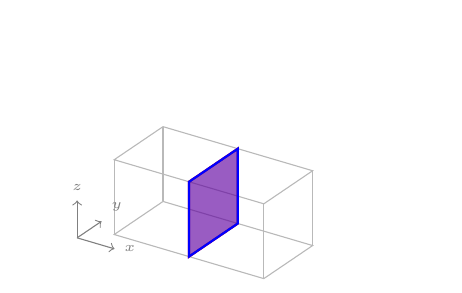
\begin{tikzpicture}[geo]\useasboundingbox (-0.7,-0.7,-0.3) rectangle (2.7,2.4,2.5); \cube{0}{0}{0}\cube{1}{0}{0} \facex{1}{0}{0}{red} \facex{1}{0}{0}{blue} \axes\end{tikzpicture} & 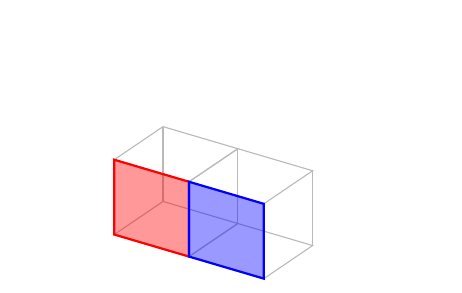
\begin{tikzpicture}[geo]\useasboundingbox (-0.7,-0.7,-0.3) rectangle (2.7,2.4,2.5); \cube{0}{0}{0}\cube{1}{0}{0} \facey{0}{0}{0}{red} \facey{0}{1}{0}{blue}\end{tikzpicture} & 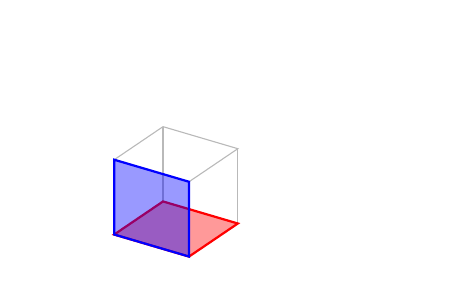
\begin{tikzpicture}[geo]\useasboundingbox (-0.7,-0.7,-0.3) rectangle (2.7,2.4,2.5); \cube{0}{0}{0} \facez{0}{0}{0}{red} \facey{0}{0}{0}{blue}\end{tikzpicture} \\[2pt]
\parbox{0.31\textwidth}{\centering\textbf{S}: coincident\\ {\scriptsize $\Delta=(1,0,0)$: yzL of target, yzU of source}} & \parbox{0.31\textwidth}{\centering\textbf{Ef}: flat edge, coplanar\\ {\scriptsize $\Delta=(1,0,0)$: xzL of target, xzL of source}} & \parbox{0.31\textwidth}{\centering\textbf{Ec}: cornered edge, perpendicular\\ {\scriptsize $\Delta=0$: xzL and xyL of the same cell}} \\[10pt]
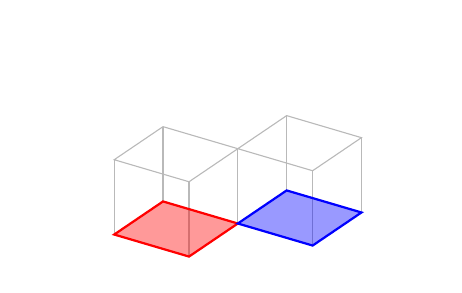
\begin{tikzpicture}[geo]\useasboundingbox (-0.7,-0.7,-0.3) rectangle (2.7,2.4,2.5); \cube{0}{0}{0}\cube{1}{1}{0} \facez{0}{0}{0}{red} \facez{0}{1}{1}{blue}\end{tikzpicture} & 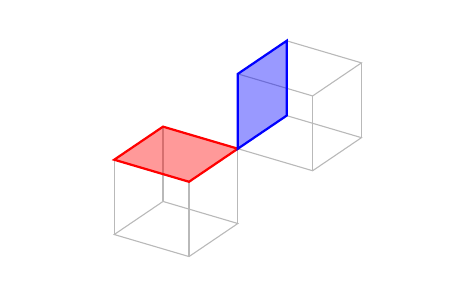
\begin{tikzpicture}[geo]\useasboundingbox (-0.7,-0.7,-0.3) rectangle (2.7,2.4,2.5); \cube{0}{0}{0}\cube{1}{1}{1} \facez{1}{0}{0}{red} \facex{1}{1}{1}{blue}\end{tikzpicture} & 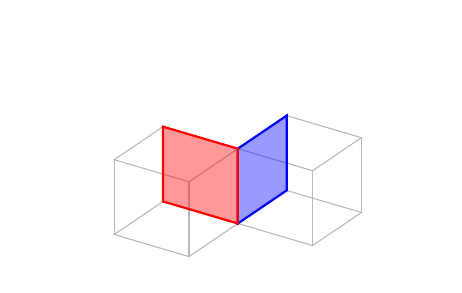
\begin{tikzpicture}[geo]\useasboundingbox (-0.7,-0.7,-0.3) rectangle (2.7,2.4,2.5); \cube{0}{0}{0}\cube{1}{1}{0} \facex{1}{1}{0}{blue} \facey{1}{0}{0}{red}\end{tikzpicture} \\[2pt]
\parbox{0.31\textwidth}{\centering\textbf{Vc}: coplanar vertex\\ {\scriptsize $\Delta=(1,1,0)$: xyL of target, xyL of source}} & \parbox{0.31\textwidth}{\centering\textbf{Vp}: perpendicular vertex\\ {\scriptsize $\Delta=(1,1,1)$: yzL of target, xyU of source}} & \parbox{0.31\textwidth}{\centering\textbf{Ec}: cornered edge across cells\\ {\scriptsize $\Delta=(1,1,0)$: yzL of target, xzU of source}} \\[10pt]
\end{tabular}\end{center}

\caption{The five contact geometries of Table~1. Red: source face $F'$ (source cell at the
origin); blue: target face $F$ (target cell displaced by $\Delta$). Where the two faces
coincide (S) the colours overlap.}
\label{fig:contact}
\end{figure}

\begin{figure}[htbp]
\begin{center}\footnotesize
\begin{tabular}{@{}ccc@{}}
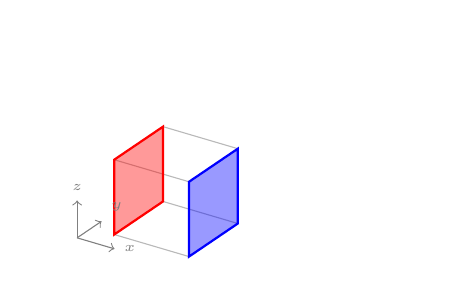
\begin{tikzpicture}[geo]\useasboundingbox (-0.7,-0.7,-0.3) rectangle (2.7,2.4,2.5); \cube{0}{0}{0} \facex{0}{0}{0}{red} \facex{1}{0}{0}{blue} \axes\end{tikzpicture} & 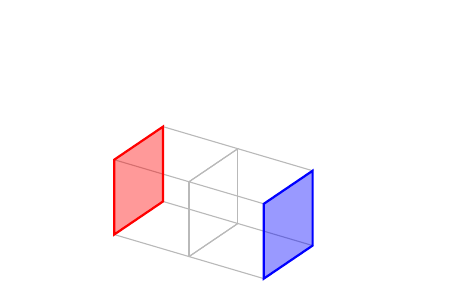
\begin{tikzpicture}[geo]\useasboundingbox (-0.7,-0.7,-0.3) rectangle (2.7,2.4,2.5); \cube{0}{0}{0}\cube{1}{0}{0} \facex{0}{0}{0}{red} \facex{2}{0}{0}{blue}\end{tikzpicture} & 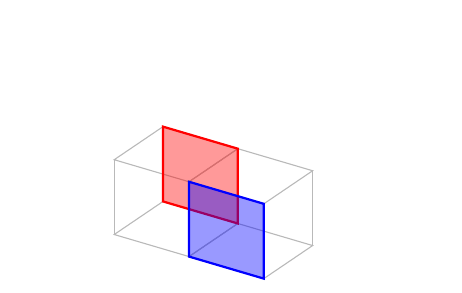
\begin{tikzpicture}[geo]\useasboundingbox (-0.7,-0.7,-0.3) rectangle (2.7,2.4,2.5); \cube{0}{0}{0}\cube{1}{0}{0} \facey{1}{0}{0}{red} \facey{0}{1}{0}{blue}\end{tikzpicture} \\[2pt]
\parbox{0.31\textwidth}{\centering\textbf{P1}: parallel, one cell apart\\ {\scriptsize $\Delta=0$: yzU of target, yzL of source}} & \parbox{0.31\textwidth}{\centering\textbf{P2}: parallel, two cells apart\\ {\scriptsize $\Delta=(1,0,0)$: yzU of target, yzL of source}} & \parbox{0.31\textwidth}{\centering\textbf{P1s}: parallel, one apart, shifted\\ {\scriptsize $\Delta=(1,0,0)$: xzL of target, xzU of source}} \\[10pt]
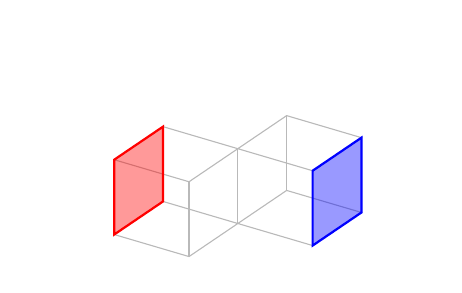
\begin{tikzpicture}[geo]\useasboundingbox (-0.7,-0.7,-0.3) rectangle (2.7,2.4,2.5); \cube{0}{0}{0}\cube{1}{1}{0} \facex{0}{0}{0}{red} \facex{2}{1}{0}{blue}\end{tikzpicture} & 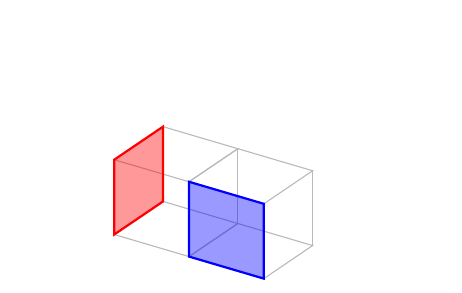
\begin{tikzpicture}[geo]\useasboundingbox (-0.7,-0.7,-0.3) rectangle (2.7,2.4,2.5); \cube{0}{0}{0}\cube{1}{0}{0} \facex{0}{0}{0}{red} \facey{0}{1}{0}{blue}\end{tikzpicture} \\[2pt]
\parbox{0.31\textwidth}{\centering\textbf{P2s}: parallel, two apart, shifted\\ {\scriptsize $\Delta=(1,1,0)$: yzU of target, yzL of source}} & \parbox{0.31\textwidth}{\centering\textbf{Xg}: perpendicular, not meeting\\ {\scriptsize $\Delta=(1,0,0)$: xzL of target, yzL of source}} \\[10pt]
\end{tabular}\end{center}

\caption{The five non-touching face-pair geometries that occur between touching cells.
Same colour convention.}
\label{fig:shell}
\end{figure}

\begin{figure}[htbp]
\begin{center}\footnotesize
\begin{tabular}{@{}ccc@{}}
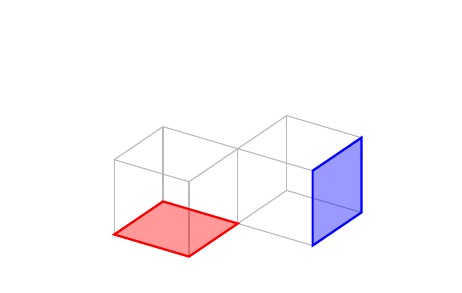
\begin{tikzpicture}[geo]\useasboundingbox (-0.7,-0.7,-0.3) rectangle (2.7,2.4,2.5); \cube{0}{0}{0}\cube{1}{1}{0} \facez{0}{0}{0}{red} \facex{2}{1}{0}{blue}\end{tikzpicture} & 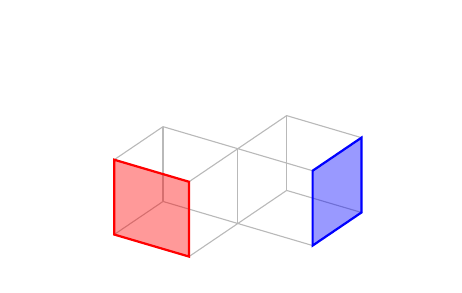
\begin{tikzpicture}[geo]\useasboundingbox (-0.7,-0.7,-0.3) rectangle (2.7,2.4,2.5); \cube{0}{0}{0}\cube{1}{1}{0} \facey{0}{0}{0}{red} \facex{2}{1}{0}{blue}\end{tikzpicture} & 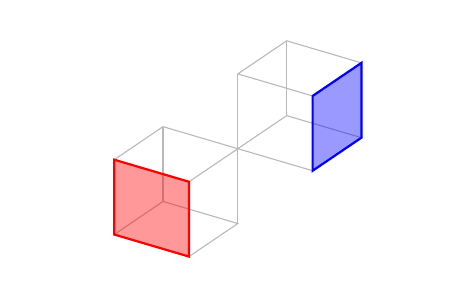
\begin{tikzpicture}[geo]\useasboundingbox (-0.7,-0.7,-0.3) rectangle (2.7,2.4,2.5); \cube{0}{0}{0}\cube{1}{1}{1} \facey{0}{0}{0}{red} \facex{2}{1}{1}{blue}\end{tikzpicture} \\[2pt]
\parbox{0.31\textwidth}{\centering\textbf{Xg-b}: perpendicular, shifted along the shared axis\\ {\scriptsize $\Delta=(1,1,0)$: yzU of target, xyL of source}} & \parbox{0.31\textwidth}{\centering\textbf{Xg-c}: perpendicular, both offsets one cell\\ {\scriptsize $\Delta=(1,1,0)$: yzU of target, xzL of source}} & \parbox{0.31\textwidth}{\centering\textbf{Xg-d}: perpendicular, both offsets one cell, shifted\\ {\scriptsize $\Delta=(1,1,1)$: yzU of target, xzL of source}} \\[10pt]
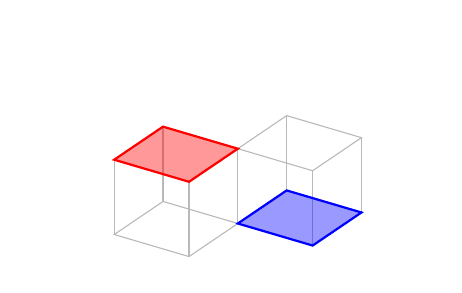
\begin{tikzpicture}[geo]\useasboundingbox (-0.7,-0.7,-0.3) rectangle (2.7,2.4,2.5); \cube{0}{0}{0}\cube{1}{1}{0} \facez{1}{0}{0}{red} \facez{0}{1}{1}{blue}\end{tikzpicture} & 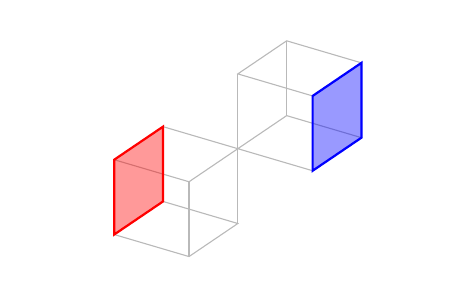
\begin{tikzpicture}[geo]\useasboundingbox (-0.7,-0.7,-0.3) rectangle (2.7,2.4,2.5); \cube{0}{0}{0}\cube{1}{1}{1} \facex{0}{0}{0}{red} \facex{2}{1}{1}{blue}\end{tikzpicture} \\[2pt]
\parbox{0.31\textwidth}{\centering\textbf{P1s-b}: parallel, one apart, doubly shifted\\ {\scriptsize $\Delta=(1,1,0)$: xyL of target, xyU of source}} & \parbox{0.31\textwidth}{\centering\textbf{P2s-b}: parallel, two apart, doubly shifted\\ {\scriptsize $\Delta=(1,1,1)$: yzU of target, yzL of source}} \\[10pt]
\end{tabular}\end{center}

\caption{The five sub-geometries that the signature classification separates from their
Table-1 parents: three further Xg classes, and the doubly shifted parallel classes.
Same colour convention.}
\label{fig:extra}
\end{figure}

\section{The coplanar and parallel-offset geometries}
\label{sec:cop}

Nine of the fifteen sub-codes are two-dimensional in the sense of \eqref{eq:pairbox}: both
panels are parallel to a common plane, the two in-plane axes carry trapezoid weights, and
the third axis contributes a frozen offset $c \in \{0, s_3, 2s_3\}$. They are S, Ef and Vc
at $c = 0$; P1, P1s and P1s-b at $c = s_3$; P2, P2s and P2s-b at $c = 2s_3$. The three
families differ only in which trapezoids appear.

\subsection{The common assembly}
\label{sec:copasm}

Write the weight of a box as $(\alpha_0 + \alpha_1 u)(\beta_0 + \beta_1 v)$ and let
\begin{equation}
C(P,Q) = \alpha_0\beta_0\,M_{00}^{(m)}(P,Q;c) + \alpha_0\beta_1\,M_{01}^{(m)}(P,Q;c)
       + \alpha_1\beta_0\,M_{10}^{(m)}(P,Q;c) + \alpha_1\beta_1\,M_{11}^{(m)}(P,Q;c),
\end{equation}
\begin{equation}
\mathcal{R}[u_1,u_2;v_1,v_2;\alpha,\beta] = C(u_2,v_2) - C(u_1,v_2) - C(u_2,v_1) + C(u_1,v_1),
\end{equation}
the corner inclusion--exclusion that turns corner moments into a moment over
$[u_1,u_2]\times[v_1,v_2]$. Then, with $p, q$ the two in-plane edge lengths, $w$ the width
across a shared edge, $e$ the shared edge length, and $a, b$ the two in-plane edges of a
corner-touching pair,
\begin{equation}
\boxed{\;
\begin{aligned}
\text{S, P1, P2}\ (c = 0,\,s_3,\,2s_3):\quad & I_m = 4\,\mathcal{R}[0,p;0,q;(p,-1),(q,-1)],\\[2pt]
\text{Ef, P1s, P2s}\ (c = 0,\,s_3,\,2s_3):\quad & I_m = 2\bigl\{\mathcal{R}[0,w;0,e;(0,1),(e,-1)]\\
 &\qquad\quad + \mathcal{R}[w,2w;0,e;(2w,-1),(e,-1)]\bigr\},\\[2pt]
\text{Vc, P1s-b, P2s-b}\ (c = 0,\,s_3,\,2s_3):\quad & I_m = \mathcal{R}[0,a;0,b;(0,1),(0,1)]\\
 &\qquad + \mathcal{R}[a,2a;0,b;(2a,-1),(0,1)]\\
 &\qquad + \mathcal{R}[0,a;b,2b;(0,1),(2b,-1)]\\
 &\qquad + \mathcal{R}[a,2a;b,2b;(2a,-1),(2b,-1)].
\end{aligned}\;}
\label{eq:copasm}
\end{equation}
The factor $4$ for S and the factor $2$ for Ef are the reflections of the difference
vector into the positive quadrant; Vc's four terms are the four quadrants of the shifted
triangle pair and carry no reflection factor, because its trapezoids are one-sided.

Two remarks. First, \emph{the three offset values are the only difference between the
three rows of Table~1 they cover}: a parallel-offset geometry is its coplanar parent with
$c\neq 0$, which enters only through the $c^2$ term of \eqref{eq:divid} and the $c$-powers
of $M_{00}$, so no new derivation is required and none was done. Second, the corner
inclusion--exclusion in $\mathcal{R}$ is a genuine source of cancellation for the shifted
boxes, and Section~\ref{sec:cancel} replaces it: the shipped code integrates each shifted
box directly rather than as a four-corner difference.

For the explicit forms it is convenient to have the four corner moments in the notation
the polar route used, with $\alpha = \sqrt{p^2+c^2}$, $\beta = \sqrt{q^2+c^2}$ and
$R = \sqrt{p^2+q^2+c^2}$:
\begin{equation}
G_{ij}(p,q;M,c) = \int_0^p\!\!\int_0^q u^i v^j (u^2+v^2+c^2)^{M/2} = M_{ij}^{(M)}(p,q;c),
\end{equation}
\begin{equation}
G_{00} = \frac{1}{M+2}\Bigl[\sum_{\substack{k\equiv M\ (2)\\ k_0\le k\le M}}
 c^{M-k}\bigl(p\,J_k(q;\alpha) + q\,J_k(p;\beta)\bigr)
 + [M\text{ odd}]\;c^{M+1}\,\Phi(p,q,c)\Bigr],
\label{eq:G00}
\end{equation}
with $k_0 = 1$ for odd $M$ and $0$ for even $M$, and
$\Phi(p,q,c) = p\asinh(q/\alpha) + q\asinh(p/\beta) - c\atan(pq/(cR))$ the rectangle
potential, which is $M_{00}^{(-1)}$ again.

\subsection{S: coincident faces}
\label{sec:S}

\geofig{\figSS}{$\Delta = (1,0,0)$: yzL of the target against yzU of the source. Panels
$A = B = [0,a]\times[0,b]\times\{0\}$.}

This is the case Section~5.2 of the companion document solved for every $m$ at once, and
it is used here as the template and as a test of the machinery rather than as new work.
The difference-variable reduction gives the bilinear weight $(p-u)(q-v)$ on the quadrant,
and in polar coordinates about the corner the radial integral is exact. With
$h = \sqrt{p^2+q^2}$ and
$\mathrm{mom}(m) = \int_0^p\!\int_0^q (p-u)(q-v)(u^2+v^2)^{m+1/2}$, so that
$I_{2m+1} = 4\,\mathrm{mom}(m)$,
{\small
\begin{equation}
\boxed{\;
\begin{aligned}
\mathrm{mom}(m) = {}& B_m\Bigl[\, p^2 q^2 \!\sum_{j=1}^{m+1} \frac{(2j-2)!!}{(2j-1)!!}\, h^{2j-1}\bigl(p^{2(m+1-j)} + q^{2(m+1-j)}\bigr)
+ p\,q^{2m+4}\asinh\frac{p}{q} + q\,p^{2m+4}\asinh\frac{q}{p} \Bigr] \\
& - \frac{h^{2m+5} - p^{2m+5} - q^{2m+5}}{(2m+3)(2m+4)(2m+5)},
\qquad
B_m = \frac{(2m+1)!!}{(2m+2)!!\,(2m+3)(2m+4)},
\end{aligned}\;}
\label{eq:momgen}
\end{equation}}%
which is equation~(31) of the companion document, and its two-term recurrence, with
$X_m(p,q) = q\,p^{2m+4}S_{2m+3}$,
\begin{equation}
X_{-1} = p^2 q\,\asinh\frac{q}{p},\qquad
X_m = \frac{p^2 q^2 h^{2m+1}}{2m+2} + \frac{2m+1}{2m+2}\,p^2 X_{m-1},
\end{equation}
\begin{equation}
\mathrm{mom}(m) = \frac{X_m(p,q) + X_m(q,p)}{(2m+3)(2m+4)} - \frac{h^{2m+5} - p^{2m+5} - q^{2m+5}}{(2m+3)(2m+4)(2m+5)} .
\end{equation}
At $m = -1$ the sum is empty and \eqref{eq:momgen} is \code{rSrfSlf}. The box route reaches
the same value from \eqref{eq:copasm} with $c = 0$; the two agree to $2.33\times10^{-90}$
over the eleven shapes and $m = -1,\ldots,12$, which is the cross-check that the general
assembly is right where the answer was already known.

\paragraph{Cancellation.} The only dangerous group is $h^{2m+5} - q^{2m+5}$, a difference
of two $O(q^{2m+5})$ numbers costing $2\log_{10}(q/p)$ digits. Written as the product
$h^n - b^n = \frac{a^2}{h+b}\sum_{i=0}^{n-1}h^i b^{n-1-i}$ with
$(a,b) = \operatorname{minmax}(p,q)$, every remaining term is positive. In the shipped
code S never reaches that expression at all: its four boxes are corner boxes of type
fall/fall at offset $c = 0$, and the box integrator handles them directly.

\paragraph{Measured.} Correctness $6.34\times10^{-44}$ (thinX, $m=-1$; reference floor),
$144$-pair sweep $1.91\times10^{-48}$, cross-check against \eqref{eq:momgen}
$2.33\times10^{-90}$. Digits lost in \code{Float64} over the $13\times14$ grid, by $m$:

\begin{center}\small
\begin{tabular}{@{}lcccccccccccccc@{}}
\toprule
$m$ & $-1$ & 0 & 1 & 2 & 3 & 4 & 5 & 6 & 7 & 8 & 9 & 10 & 11 & 12\\
\midrule
S & 0.30 & 0.00 & 0.07 & 0.00 & 0.00 & 0.00 & 0.29 & 0.00 & 0.30 & 0.00 & 0.30 & 0.05 & 0.40 & 0.39\\
\bottomrule
\end{tabular}
\end{center}
\noindent
worst $0.40$ at $(a/b, c/b) = (10^{3}, 10^{-6})$, $m = 11$. Against Gila: the series
reproduces \code{wekS} to $6.30\times10^{-11}$ at \code{intOrd} $48$ and
$1.37\times10^{-11}$ at $64$ (worst over the cell scales carrying both orders), and
$I_{-1}$ agrees with $4\pi f^2\,\code{rSrfSlf}$ to $2.51\times10^{-16}$.

\subsection{Ef: coplanar, sharing an edge}
\label{sec:Ef}

\geofig{\figEf}{$\Delta = (1,0,0)$: xzL of the target against xzL of the source. Panels
$A = [0,a]\times[0,b]\times\{0\}$, $B = [a,2a]\times[0,b]\times\{0\}$; shared edge $b$,
width $a$.}

In the direction across the shared edge the convolution weight is the triangle
$a - |u - a|$ on $(0,2a)$, and in the direction along it the triangle $b - |v|$. Splitting
at $u = a$ gives the two boxes of the middle row of \eqref{eq:copasm}: weight $u\,(b-v)$
on $[0,a]\times[0,b]$ and weight $(2a-u)(b-v)$ on $[a,2a]\times[0,b]$. Both are the
corner moments $M_{ij}$, and at $m = -1$ collecting terms gives \code{rSrfEdgFlt},
equation~(17) of the companion document,
\begin{equation}
\boxed{\;
I_{-1}(\text{Ef}) = \tfrac{1}{3}\bigl[Q + 6\,a^2 b\,D_1 + 6\,a b^2\,D_2\bigr],\;}
\qquad
\begin{aligned}
Q &= 2h_1^3 - h_2^3 - a^3 + 6b^3,\\
D_1 &= \asinh\tfrac{2b}{a} - \asinh\tfrac{b}{a},\\
D_2 &= 2\asinh\tfrac{a}{2b} - \asinh\tfrac{a}{b},
\end{aligned}
\end{equation}
with $h_1 = \sqrt{a^2+b^2}$, $h_2 = \sqrt{a^2+4b^2}$. (The companion document's
\code{rSrfEdgFlt} carries the kernel's $1/(4\pi f^2)$; here $I_{-1}$ is the bare integral,
so the prefactor is $1/3$ rather than $1/(12\pi f^2)$.) For general $m$ there is no reason
to collect: the assembly \eqref{eq:copasm} with the general-$m$ $G_{ij}$ of
\eqref{eq:G00}--\eqref{eq:M1011} is a closed form for every integer $m \ge -1$, and it is
what the code evaluates.

\paragraph{Cancellation.} As written the collected $m = -1$ form cancels catastrophically
when $a \ll b$: $Q$ is $O(a^3b^2/b^3)$ out of terms of size $b^3$, and the two $\asinh$
differences are small differences of large logarithms. The remedies are the companion
document's: write $Q$ as a manifestly negative product and each difference as
$\log(1+x)$ with $x$ a ratio of positive quantities. The shipped code again does not use
the collected form; its two box types (fall$_1$/fall$_0$ and rise$_0$/fall$_0$) are
integrated directly.

\paragraph{Measured.} Correctness $3.82\times10^{-44}$ (thinX, $m=-1$), $144$-pair sweep
$1.44\times10^{-48}$, cross-check against the polar explicit form $8.10\times10^{-90}$,
and against \code{rSrfEdgFlt} at $m = -1$, $1.9\times10^{-84}$.

\begin{center}\small
\begin{tabular}{@{}lcccccccccccccc@{}}
\toprule
$m$ & $-1$ & 0 & 1 & 2 & 3 & 4 & 5 & 6 & 7 & 8 & 9 & 10 & 11 & 12\\
\midrule
Ef & 0.05 & 0.00 & 0.00 & 0.05 & 0.24 & 0.03 & 0.03 & 0.14 & 0.17 & 0.09 & 0.21 & 0.34 & 0.37 & 0.26\\
\bottomrule
\end{tabular}
\end{center}
\noindent
worst $0.37$ at $(10^{3}, 10^{-6})$, $m = 11$. Against Gila: \code{wekE} entries 1--6
agree with the series to $2.90\times10^{-10}$ at \code{intOrd} $48$ and
$1.92\times10^{-11}$ at $64$; $I_{-1}$ against $4\pi f^2\,\code{rSrfEdgFlt}$ is
$1.02\times10^{-16}$. Ef is also the one entry where Gila's order refinement moves the
wrong way on the slender cell (Section~\ref{sec:gila}).

\subsection{Vc: coplanar, sharing only a corner}
\label{sec:Vc}

\geofig{\figVc}{$\Delta = (1,1,0)$: xyL of the target against xyL of the source. Panels
$A = [0,a]\times[0,b]\times\{0\}$, $B = [a,2a]\times[b,2b]\times\{0\}$.}

Both in-plane weights are shifted triangles, so the four quadrants of \eqref{eq:copasm}
all survive and none of them touches the origin except at one corner. Nothing was known
about this geometry before; it now has an explicit closed form for every $m$, obtained
independently by the polar route and by numerical discovery with exact coefficient
recovery. With $h_{ab} = \sqrt{a^2+b^2}$, $h_{a2b} = \sqrt{a^2+4b^2}$,
$h_{2ab} = \sqrt{4a^2+b^2}$ and $\lambda_m = m!!/(m+1)!!$,
{\small
\begin{equation}
\boxed{\;
\begin{aligned}
I_m(\text{Vc}) = {}& \frac{\lambda_m\,a^{m+3}b}{(m+2)(m+3)}\Bigl[(2^{m+4}+4)\asinh\tfrac{b}{a}
 - 2^{m+4}\asinh\tfrac{b}{2a} - 4\asinh\tfrac{2b}{a}\Bigr] \;+\; (a\leftrightarrow b)\\
&+ \frac{2}{(m+2)(m+3)(m+4)}\Bigl[-(2^{m+3}-1)(a^{m+4}+b^{m+4})\\
&\hphantom{+\frac{2}{(m+2)(m+3)(m+4)}\Bigl[}
 - (2^{m+3}+2)\,\hat G_m(a,b) + \hat G_m(a,2b) + \hat G_m(2a,b)\Bigr],
\end{aligned}\;}
\label{eq:vcgen}
\end{equation}}%
where $\hat G_m$ is a universal ``hypotenuse polynomial'' in $h = \sqrt{a^2+b^2}$ and
$s = a^2b^2$,
\begin{equation}
\hat G_{-1} = h^3,\quad
\hat G_{1} = (h^4 - 5s)h,\quad
\hat G_{3} = \bigl(h^6 - \tfrac{49}{8}s h^2\bigr)h,\quad
\hat G_{5} = \bigl(h^8 - \tfrac{123}{16}s h^4 + \tfrac{45}{8}s^2\bigr)h,
\end{equation}
the $m = 7$ member having been confirmed out of sample. Specializing,
\begin{align}
I_{-1}(\text{Vc}) &= 2a^2b\Bigl[3\asinh\tfrac{b}{a} - 2\asinh\tfrac{b}{2a} - \asinh\tfrac{2b}{a}\Bigr]
 + 2ab^2\Bigl[3\asinh\tfrac{a}{b} - 2\asinh\tfrac{a}{2b} - \asinh\tfrac{2a}{b}\Bigr]\notag\\
&\qquad - (a^3+b^3) - 2h_{ab}^3 + \tfrac{1}{3}\bigl(h_{a2b}^3 + h_{2ab}^3\bigr),
\label{eq:vcm1}\\
I_{1}(\text{Vc}) &= a^4b\Bigl[\tfrac{3}{2}\asinh\tfrac{b}{a} - \tfrac{4}{3}\asinh\tfrac{b}{2a} - \tfrac16\asinh\tfrac{2b}{a}\Bigr] + (a\leftrightarrow b)\notag\\
&\qquad - \tfrac12(a^5+b^5) - \tfrac35 h_{ab}^5 + 3s\,h_{ab} + \tfrac{1}{30}\bigl(h_{a2b}^5 + h_{2ab}^5\bigr) - \tfrac23 s\bigl(h_{a2b} + h_{2ab}\bigr),\\
I_{3}(\text{Vc}) &= a^6b\Bigl[\tfrac{33}{20}\asinh\tfrac{b}{a} - \tfrac85\asinh\tfrac{b}{2a} - \tfrac1{20}\asinh\tfrac{2b}{a}\Bigr] + (a\leftrightarrow b)\notag\\
&\qquad - \tfrac35(a^7+b^7) - \tfrac{22}{35}h_{ab}^7 + \tfrac{77}{20}s\,h_{ab}^3 + \tfrac1{105}\bigl(h_{a2b}^7 + h_{2ab}^7\bigr) - \tfrac{7}{30}s\bigl(h_{a2b}^3 + h_{2ab}^3\bigr),
\end{align}
with $s = a^2b^2$. Equation~\eqref{eq:vcm1} is \eqref{eq:vcgen} at $m = -1$ term by term;
the two were derived independently and the agreement of the $\lambda_{-1} = 1$,
$(m+2)(m+3) = 2$ specialization with the discovered coefficients is one of the reasons to
trust the general formula. The atom set of Vc has six members and never changes with $m$;
only the coefficients do, and they are homogeneous of degree $m+3$.

\paragraph{Verification of the coefficients.} All $259$ rational coefficients of the
explicit Vc, Vp and Xg forms at $m = -1, 1, 3$ were recovered independently from
\code{pairMom} data by solving a linear system in the conjectured atom basis, with
residuals between $3.9\times10^{-30}$ and $1.8\times10^{-53}$: Vc needs $14$, $17$ and
$20$ terms at those three $m$. This is a genuinely independent confirmation of the algebra,
since the coefficients come from numbers, not from the derivation.

\paragraph{Cancellation.} As written, \eqref{eq:vcgen} loses up to $11.7$ digits at
$b/a = 10^{\pm 6}$, and the top-level amplification explains all of it: there are four
algebraic buckets $a^{m+4}+b^{m+4}$, $h_{ab}$, $h_{a2b}$, $h_{2ab}$, each of size
$O(a^{m+4})$, against an integral of size $O(a^{m+2}b^2)$; the $\asinh$ block is already a
second difference and is fine. The shipped code does not use \eqref{eq:vcgen}: Vc's four
boxes are integrated directly, and its four box types include the doubly shifted
fall$_1$/fall$_1$ that motivated the whole of Section~\ref{sec:cancel}.

\paragraph{Measured.} Correctness $2.43\times10^{-45}$ (sliver, $m=-1$), $144$-pair sweep
$1.37\times10^{-48}$, cross-check against the polar form $9.01\times10^{-90}$ and against
the discovery form $6.95\times10^{-90}$.

\begin{center}\small
\begin{tabular}{@{}lcccccccccccccc@{}}
\toprule
$m$ & $-1$ & 0 & 1 & 2 & 3 & 4 & 5 & 6 & 7 & 8 & 9 & 10 & 11 & 12\\
\midrule
Vc & 0.08 & 0.00 & 0.04 & 0.00 & 0.17 & 0.17 & 0.00 & 0.17 & 0.26 & 0.05 & 0.13 & 0.23 & 0.19 & 0.23\\
\bottomrule
\end{tabular}
\end{center}
\noindent
worst $0.26$ at $(10^{-1}, 10^{-6})$, $m = 7$; the best-conditioned code in the whole set,
which is worth contrasting with the $11.7$ digits of the explicit form. Against Gila:
\code{wekV} entries 1--3 agree with the series to $4.98\times10^{-10}$ at \code{intOrd}
$48$ and $8.99\times10^{-11}$ at $64$. Gila has no closed form for Vc, so there is no
$m = -1$ static-part check; the series is the first exact value this geometry has had.

\subsection{P1 and P2: parallel, aligned}
\label{sec:P12}

\geofig{\figPa\qquad\figPb}{Left, P1 at $\Delta = 0$: yzU of the target against yzL of the
source, one cell length apart. Right, P2 at $\Delta = (1,0,0)$, two cell lengths apart.
Panels $A = [0,a]\times[0,b]\times\{0\}$, $B = [0,a]\times[0,b]\times\{c\}$ or
$\{2c\}$.}

These are S with a frozen offset. The assembly is the first row of \eqref{eq:copasm} with
$c = s_3$ and $c = 2s_3$, and the closed form is \eqref{eq:G00} together with
\eqref{eq:M1011}: the $c$-powers and the $\atan$ term of $\Phi$ are the whole difference
from the self face. Explicitly, for every integer $m\ge -1$,
\begin{equation}
\boxed{\;
I_m(\text{P1}) = 4\,\mathcal{R}[0,a;0,b;(a,-1),(b,-1)] \text{ at } c = s_3,
\qquad
I_m(\text{P2}) = \text{the same at } c = 2s_3 . \;}
\end{equation}
Both are separated pairs: $r$ never vanishes on the domain, so there is no singular
behaviour to arrange around, and the difficulty is purely one of conditioning.

\paragraph{Cancellation.} These two geometries are where the naive route fails worst.
Written through \eqref{eq:M1011}, the P family loses up to $29$ digits, and the culprit is
$M_{11}$ alone: its numerator $R^{p} - d_A^{p} - d_B^{p} + c^{p}$ with $p = m+4$ is a
four-term difference in which, when $c \gg a, b$, all four terms are within
$O((a^2+b^2)/c^2)$ of $c^{p}$ while the true value is $p(p-2)a^2b^2c^{p-4}/4$, so about
$2\log_{10}(c/a) + 2\log_{10}(c/b)$ digits vanish. Measured, $M_{11}$ loses $28.4$ digits
at $(a,b,c,m) = (0.01, 1, 10^{6}, -1)$, and the assembled P1 loses \emph{exactly} the same
$28.4$ at the same point: the whole P-family loss is $M_{11}$ and nothing else. $M_{00}$
by contrast loses $0.9$ digits over the entire grid. The shipped code removes this
completely by never forming $M_{11}$: it integrates each box against its own weight with
the ladder of Section~\ref{sec:cancel2}, and for boxes far from the origin --- which is
exactly the regime $c \gg a,b$ --- it uses the centred Taylor expansion.

\paragraph{Measured.} Correctness $4.50\times10^{-60}$ (P1, fatZ, $m=1$) and
$3.84\times10^{-60}$ (P2, fatX, $m=11$); note that these are three orders of magnitude
below the touching geometries, because \code{pairMom} converges much faster on a separated
pair. $144$-pair sweep $1.12\times10^{-75}$ (P1) and $9.31\times10^{-76}$ (P2).
Cross-checks against the polar explicit forms $1.26\times10^{-84}$ and
$2.24\times10^{-83}$, the worst at fatZ, $m=-1$, where the explicit form is itself
cancelling.

\begin{center}\small
\begin{tabular}{@{}lcccccccccccccc@{}}
\toprule
$m$ & $-1$ & 0 & 1 & 2 & 3 & 4 & 5 & 6 & 7 & 8 & 9 & 10 & 11 & 12\\
\midrule
P1 & 0.48 & 0.00 & 0.29 & 0.12 & 0.41 & 0.24 & 0.36 & 0.45 & 0.42 & 0.44 & 0.46 & 0.53 & 0.60 & 0.53\\
P2 & 0.62 & 0.00 & 0.20 & 0.23 & 0.19 & 0.24 & 0.29 & 0.39 & 0.37 & 0.55 & 0.47 & 0.55 & 0.60 & 0.59\\
\bottomrule
\end{tabular}
\end{center}
\noindent
worst $0.60$ (P1) at $(10^{-2}, 10^{-3})$, $m = 11$ and $0.62$ (P2) at
$(10^{-6}, 10^{-1})$, $m = -1$ --- against $28.4$ and $25.4$ for the plain closed form.
Against Gila: the order-9 fixed rule reproduces the series to $8.9\times10^{-14}$ (P1) and
$1.1\times10^{-15}$ (P2) at a $(1/32)^3$ cell, and P1 is the one code where that rule
fails outright on a slender cell, at $1.57\times10^{-2}$ (Section~\ref{sec:gila}).

\subsection{P1s and P2s: parallel, laterally shifted}
\label{sec:P12s}

\geofig{\figPas\qquad\figPbs}{Left, P1s at $\Delta = (1,0,0)$: xzL of the target against
xzU of the source. Right, P2s at $\Delta = (1,1,0)$: yzU against yzL. Panels
$A = [0,a]\times[0,b]\times\{0\}$, $B = [a,2a]\times[0,b]\times\{c\}$ or $\{2c\}$.}

Ef with a frozen offset: one in-plane axis carries the shifted triangle of the flat edge,
the other the centred triangle of the self face. The assembly is the middle row of
\eqref{eq:copasm} at $c = s_3$ and $c = 2s_3$, and the closed form is again
\eqref{eq:G00}--\eqref{eq:M1011}.

\paragraph{Cancellation.} Two mechanisms combine here, and P1s was the geometry that
exposed the second. As for P1/P2, $M_{11}$ costs up to $28.3$ digits as written. On top of
that, the shifted box $[a,2a]$ carries the corner amplification $u_2/(u_2-u_1) = 2$ per
shifted axis, which was measured exactly: for the fall/fall box type the ratio
$|u_2v_2M_{00}|/|W|$ tends to $u_2v_2/(h_uh_v)$, equal to $4$ for a corner box, $8$ with
one shifted axis and $16$ with two. With the closed forms alone P1s and P2s stalled at
$1.15$ and $1.27$ digits at $m = -1$, above the bar; the centred Taylor branch of
Section~\ref{sec:cancel2} brings them to $0.64$ and $0.63$.

\paragraph{Measured.} Correctness $4.53\times10^{-60}$ (P1s, fatZ, $m=9$) and
$4.01\times10^{-60}$ (P2s, small, $m=7$); $144$-pair sweep $9.44\times10^{-76}$ and
$4.72\times10^{-76}$; cross-checks against the polar forms $5.27\times10^{-85}$ and
$5.60\times10^{-84}$.

\begin{center}\small
\begin{tabular}{@{}lcccccccccccccc@{}}
\toprule
$m$ & $-1$ & 0 & 1 & 2 & 3 & 4 & 5 & 6 & 7 & 8 & 9 & 10 & 11 & 12\\
\midrule
P1s & 0.64 & 0.00 & 0.24 & 0.17 & 0.32 & 0.27 & 0.42 & 0.43 & 0.42 & 0.54 & 0.53 & 0.54 & 0.54 & 0.62\\
P2s & 0.63 & 0.00 & 0.17 & 0.25 & 0.32 & 0.25 & 0.41 & 0.41 & 0.54 & 0.55 & 0.54 & 0.54 & 0.61 & 0.63\\
\bottomrule
\end{tabular}
\end{center}
\noindent
worst $0.64$ (P1s) at $(10^{-2}, 10^{-1})$, $m = -1$ and $0.63$ (P2s) at
$(10^{4}, 10^{-4})$, $m = 12$. Against Gila's order-9 rule at a $(1/32)^3$ cell:
$2.1\times10^{-14}$ (P1s) and $5.7\times10^{-15}$ (P2s); on the slender cell P1s degrades
to $2.81\times10^{-4}$ while P2s stays at $4.3\times10^{-15}$, which is the expected
pattern (the failure is driven by the \emph{gap} being the short edge, and P2s's gap is
two short edges).

\subsection{P1s-b and P2s-b: parallel, doubly shifted}
\label{sec:P12sb}

\geofig{\figPasb\qquad\figPbsb}{Left, P1s-b at $\Delta = (1,1,0)$: xyL of the target
against xyU of the source. Right, P2s-b at $\Delta = (1,1,1)$: yzU against yzL. Panels
$A = [a,2a]\times[b,2b]\times\{0\}$ against $B = [0,a]\times[0,b]\times\{c\}$, and the
analogue at $2c$.}

Both in-plane axes are shifted, where P1s and P2s shift one and leave the other fully
overlapping. Structurally these are \emph{Vc with a frozen offset}: the assembly is the
third row of \eqref{eq:copasm} at $c = s_3$ and $c = 2s_3$, and the four boxes are the four
quadrants of two shifted triangles. Table~1 of the companion document does not distinguish
them from P1s and P2s, which is why they carry the ``-b'' suffix.

These two sub-codes are the only ones in the set with \emph{no independent explicit closed
form}. The polar corner moments $G_{ij}$ already carry $c$, so extending
\eqref{eq:copasm}'s Vc row to $c\neq 0$ is immediate in principle, but no separate
explicit routine was written or cross-checked, and table (c) of the verification
accordingly reports ``no explicit form'' for them. Their evidence is instead: the
$320$-bit reference cache at eleven shapes (table (a)), the $144$-pair sweep against
\code{pairMom} (table (b)), homogeneity, orientation invariance under all six axis
permutations, and the $a\leftrightarrow b$ symmetry --- which they possess, at
$1.33\times10^{-96}$ and $8.65\times10^{-97}$, and P1s and P2s do \emph{not} ($0.99$ and
$0.84$). That last check is the discriminating one: it shows the shifted codes are not
being silently confused with their unshifted parents.

\paragraph{Cancellation.} Their fall$_1$/fall$_1$ box is the worst-conditioned box type in
the two-dimensional set, amplification exactly $16$, and with closed forms only they lost
$1.24$ and $1.38$ digits at $m = -1$. The centred Taylor branch covers that box type in
\emph{every} cell of the grid, at most $42$ levels deep with condition number $1.26$, and
brings them to $0.34$ and $0.28$.

\paragraph{Measured.} Correctness $4.85\times10^{-60}$ (P1s-b, fatZ, $m=1$) and
$4.46\times10^{-60}$ (P2s-b, fatX, $m=1$); $144$-pair sweep $6.42\times10^{-76}$ and
$5.97\times10^{-76}$.

\begin{center}\small
\begin{tabular}{@{}lcccccccccccccc@{}}
\toprule
$m$ & $-1$ & 0 & 1 & 2 & 3 & 4 & 5 & 6 & 7 & 8 & 9 & 10 & 11 & 12\\
\midrule
P1s-b & 0.34 & 0.00 & 0.17 & 0.14 & 0.14 & 0.29 & 0.31 & 0.44 & 0.45 & 0.34 & 0.43 & 0.51 & 0.60 & 0.55\\
P2s-b & 0.28 & 0.00 & 0.13 & 0.13 & 0.14 & 0.18 & 0.37 & 0.38 & 0.38 & 0.54 & 0.50 & 0.58 & 0.58 & 0.60\\
\bottomrule
\end{tabular}
\end{center}
\noindent
worst $0.60$ (P1s-b) at $(10^{0}, 10^{-3})$, $m = 11$ and $0.60$ (P2s-b) at
$(10^{-3}, 10^{-3})$, $m = 12$. Against Gila's order-9 rule at a $(1/32)^3$ cell,
$9.9\times10^{-15}$ and $1.9\times10^{-15}$; on the slender cell, $1.80\times10^{-7}$ and
$1.28\times10^{-8}$.

\section{The perpendicular geometries}
\label{sec:prp}

Six sub-codes are three-dimensional in the sense of \eqref{eq:pairbox}: the two panels lie
in perpendicular planes, so only the shared axis admits a difference variable and carries a
trapezoid, while the two normal axes keep their own coordinates and contribute indicators.
They are Ec, Vp, Xg, Xg-b, Xg-c and Xg-d. These are the hard cases, and they were attacked
by three families independently.

\subsection{The master reduction}
\label{sec:prpasm}

Put the shared axis along $s$, with half-width $a$ and triangle centre
$\delta\in\{0,\pm a\}$, and let the two normal axes carry the indicator ranges
$[\beta_1,\beta_2]$ and $[\gamma_1,\gamma_2]$, each of which is $[0,L]$ (the panels'
projections meet) or $[L,2L]$ (they are a cell apart). With
$\Psi_m(u;B,C) = \int_0^B\!\int_0^C (u^2+v^2+w^2)^{m/2}$ and $P_m$ of \eqref{eq:P},
\begin{equation}
\boxed{\;
I_m \;=\; \sum_{i,j\in\{1,2\}} (-1)^{i+j}\,W_m(\beta_i,\gamma_j),
\qquad
W_m(B,C) = \begin{cases}
2P_m(a;B,C), & \delta = 0,\\[2pt]
P_m(2a;B,C) - 2P_m(a;B,C), & \delta = \pm a,
\end{cases}\;}
\label{eq:prpmaster}
\end{equation}
with $W_m(0,\cdot) = W_m(\cdot,0) = 0$. This single formula covers every perpendicular
face pair of Table~1 including the Xg variants with a shifted weight and both ranges
offset, which need all eight $P_m$ terms. The named orientations are
\begin{equation}
\begin{aligned}
\text{Ec}/x &: 2P_m(a;b,c), &\qquad \text{Ec}/y &: 2P_m(b;a,c),\\
\text{Vp}/x &: P_m(2b;a,c) - 2P_m(b;a,c), &\qquad \text{Vp}/y &: P_m(2a;b,c) - 2P_m(a;b,c),\\
\text{Xg}/y &: 2\bigl[P_m(a;2b,c) - P_m(a;b,c)\bigr], &\qquad \text{Xg}/x &: 2\bigl[P_m(b;2a,c) - P_m(b;a,c)\bigr],
\end{aligned}
\label{eq:prpnamed}
\end{equation}
and Xg-b, Xg-c, Xg-d are \eqref{eq:prpmaster} with $(\delta = \pm a$, one range offset$)$,
$(\delta = 0$, both offset$)$ and $(\delta = \pm a$, both offset$)$ respectively.

The primitives are the ladder of Section~\ref{sec:ladder}. Recorded here in the form the
box-potential route wrote them, with $\rho = \sqrt{t^2+B^2}$, $\sigma = \sqrt{t^2+C^2}$,
$R = \sqrt{t^2+B^2+C^2}$:
\begin{equation}
\boxed{\;
\begin{aligned}
\Psi_n(t;B,C) &= \frac{B\,J_n(C;\rho) + C\,J_n(B;\sigma) + n\,t^2\,\Psi_{n-2}}{n+2},\qquad \Psi_0 = BC,\\
\Psi_{-1}(t;B,C) &= B\asinh\frac{C}{\rho} + C\asinh\frac{B}{\sigma} - t\atan\frac{BC}{tR},\\
K^{(m)}(A,B,C) &= \frac{A\,\Psi_m(A;B,C) + B\,\Psi_m(B;A,C) + C\,\Psi_m(C;A,B)}{m+3},\\
P_m(T;B,C) &= T\,K^{(m)}(T,B,C) - \frac{\Psi_{m+2}(T;B,C) - \Psi_{m+2}(0;B,C)}{m+2}.
\end{aligned}\;}
\label{eq:prpprim}
\end{equation}
Unrolled at odd order, with $G_j = B\,J_{2j-1}(C;\rho) + C\,J_{2j-1}(B;\sigma)$,
\begin{equation}
\Psi_{2q-1}(t;B,C) = \frac{t^{2q}\Psi_{-1} + \sum_{j=1}^{q} t^{2(q-j)}G_j}{2q+1},
\end{equation}
the first three $G_j$ being, with $\alpha = \asinh(C/\rho)$ and $\beta = \asinh(B/\sigma)$,
\begin{equation}
\begin{aligned}
G_1 &= \tfrac12(B\rho^2\alpha + C\sigma^2\beta) + BCR,\\
G_2 &= \tfrac38(B\rho^4\alpha + C\sigma^4\beta) + \tfrac38 BCR(\rho^2+\sigma^2) + \tfrac12 BCR^3,\\
G_3 &= \tfrac{5}{16}(B\rho^6\alpha + C\sigma^6\beta) + \tfrac{5}{16}BCR(\rho^4+\sigma^4) + \tfrac{5}{24}BCR^3(\rho^2+\sigma^2) + \tfrac13 BCR^5 .
\end{aligned}
\end{equation}
The corner box moment at the first two odd orders, with $\alpha_c = \asinh(c/h_{ab})$ and
its mirrors and $\tau_a = \atan(bc/(aR))$ and its mirrors, is
\begin{align}
K^{(1)} &= \tfrac{1}{12}\Bigl[2ab\,h_{ab}^2\alpha_c + 2ac\,h_{ac}^2\alpha_b + 2bc\,h_{bc}^2\alpha_a
 + 3abcR - a^4\tau_a - b^4\tau_b - c^4\tau_c\Bigr],\\
K^{(3)} &= \tfrac{1}{30}\Bigl[ab\bigl(\tfrac54 h_{ab}^4 + a^4 + b^4\bigr)\alpha_c
 + ac\bigl(\tfrac54 h_{ac}^4 + a^4 + c^4\bigr)\alpha_b
 + bc\bigl(\tfrac54 h_{bc}^4 + b^4 + c^4\bigr)\alpha_a\notag\\
&\hphantom{= \tfrac{1}{30}\Bigl[} + 4abcR^3 - a^6\tau_a - b^6\tau_b - c^6\tau_c\Bigr].
\end{align}

Verification of the master formula on its own terms, before any assembly: all $24$
perpendicular face pairs at each of four offsets, cell $(3/2, 1, 2/5)$, $m = -1,\ldots,8$
--- $960$ values, maximum relative error $1.53\times10^{-51}$ against \code{pairMom}.

\subsection{Ec: perpendicular, sharing an edge}
\label{sec:Ec}

\geofig{\figEc\qquad\figEcx}{Left, Ec within one cell: xzL and xyL of the same cell. Right,
Ec across cells at $\Delta = (1,1,0)$: yzL of the target against xzU of the source. Panels
$A = [0,a]\times[0,b]\times\{0\}$, $B = [0,a]\times\{b\}\times[0,c]$; shared edge $a$,
widths $b$ and $c$.}

The shared axis carries the centred triangle $(a-|u|)$, so
$\delta = 0$ and both indicator ranges start at zero: \eqref{eq:prpmaster} collapses to a
single term, $I_m = 2P_m(a;b,c)$, and the boxed formula is \eqref{eq:P} with
\eqref{eq:prpprim}. Collected at the first three odd orders, with
$\Delta_b = \asinh(c/b) - \asinh(c/h_{ab})$ and
$\Delta_c = \asinh(b/c) - \asinh(b/h_{ac})$,
{\small
\begin{align}
P_{-1}(a;b,c) &= \tfrac{b^3}{6}\Delta_b + \tfrac{c^3}{6}\Delta_c
 + \tfrac{a^2b}{2}\alpha_c + \tfrac{a^2c}{2}\alpha_b + abc\,\alpha_a
 - \tfrac{a^3}{6}\tau_a - \tfrac{ab^2}{2}\tau_b - \tfrac{ac^2}{2}\tau_c
 - \frac{a^2bc}{3(h_{bc}+R)},
\label{eq:Pm1}\\
P_{1}(a;b,c) &= \tfrac{1}{120}\Bigl[3b^5\Delta_b + 3c^5\Delta_c
 + 5a^2b(a^2+2b^2)\alpha_c + 5a^2c(a^2+2c^2)\alpha_b + 20abc\,h_{bc}^2\alpha_a\notag\\
&\hphantom{= \tfrac{1}{120}\Bigl[}
 - 2a^5\tau_a - 10ab^4\tau_b - 10ac^4\tau_c + 19a^2bcR - 7bc\,(R^3 - h_{bc}^3)\Bigr],\\
P_{3}(a;b,c) &= \tfrac{1}{1680}\Bigl[15b^7\Delta_b + 15c^7\Delta_c
 + 7a^2b(3a^4+5a^2b^2+9b^4)\alpha_c + 7a^2c(3a^4+5a^2c^2+9c^4)\alpha_b\notag\\
&\hphantom{= \tfrac{1}{1680}\Bigl[}
 + 14abc(5h_{bc}^4 + 4b^4 + 4c^4)\alpha_a - 8a^7\tau_a - 56ab^6\tau_b - 56ac^6\tau_c\notag\\
&\hphantom{= \tfrac{1}{1680}\Bigl[}
 + bc\bigl(172a^2R^3 - 66a^4R - 15\bigl[R(h_{ab}^4+h_{ac}^4) - h_{bc}(b^4+c^4)\bigr] - 26(R^5 - h_{bc}^5)\bigr)\Bigr].
\end{align}}%
Equation~\eqref{eq:Pm1} is \code{rSrfEdgCrn} (equation~(23) of the companion document)
term for term, which is how the identity \eqref{eq:P} was first confirmed: the grouping of
the $b^3$ and $c^3$ logarithms into $\Delta_b$ and $\Delta_c$, which the companion document
found by hand and called the essential step, falls out of \eqref{eq:P} automatically. At
$m = -1$ the new form and \code{rSrfEdgCrn} agree to $1.2\times10^{-88}$.

Ec is symmetric in $b\leftrightarrow c$, and that symmetry is what \code{wekE}'s
two-orientation average relies on. It was computed, not assumed: $3.8\times10^{-96}$ over
all shapes and all $m$, and correspondingly the two orientations Gila averages give
bit-identical closed-form moments (relative difference exactly $0$ at all four cell scales).

\paragraph{Cancellation.} The entire loss of the naive route is the difference
$\Psi_{m+2}(T) - \Psi_{m+2}(0)$ in \eqref{eq:P}, whose amplification reaches $10^{11}$ to
$10^{23}$. Propagating that difference by its own recurrence, rather than forming the two
$\Psi$'s and subtracting, takes Ec from $15.7$ digits lost to $1.2$--$1.3$; the shipped
code goes further and never performs the $TK - \Delta\Psi$ split at all, integrating the
weighted box directly by $\nabla\cdot(f X r^m)$ with $f = q-u$ (Section~\ref{sec:cancel3}),
which removes the fixed factor-3 amplification of that split.

\paragraph{Measured.} Correctness $7.35\times10^{-44}$ (fatX, $m=-1$) --- the worst entry
of the whole correctness table, and it is the reference's floor, not the formula's:
recomputing \code{pairMom} at three increasing order sets at this shape gives
$1.46\times10^{-22}$, $2.64\times10^{-30}$, $7.35\times10^{-44}$. $144$-pair sweep
$4.84\times10^{-49}$; cross-check against the master formula $1.16\times10^{-95}$.

\begin{center}\small
\begin{tabular}{@{}lcccccccccccccc@{}}
\toprule
$m$ & $-1$ & 0 & 1 & 2 & 3 & 4 & 5 & 6 & 7 & 8 & 9 & 10 & 11 & 12\\
\midrule
Ec & 0.17 & 0.01 & 0.15 & 0.41 & 0.30 & 0.28 & 0.43 & 0.46 & 0.49 & 0.54 & 0.72 & 0.67 & 0.74 & 0.77\\
\bottomrule
\end{tabular}
\end{center}
\noindent
worst $0.77$ at $(10^{-3}, 10^{0})$, $m = 12$. Ec is also the code that first exceeds the
one-digit bar above $m = 12$: $1.15$ digits at $m = 25$ and $1.28$ at $m = 30$
(Section~\ref{sec:highm}). Against Gila: \code{wekE} entries 7--9 agree with the series to
$9.29\times10^{-11}$ at \code{intOrd} $48$ and $6.06\times10^{-12}$ at $64$; $I_{-1}$
against $4\pi f^2\,\code{rSrfEdgCrn}$ is $2.54\times10^{-16}$.

\subsection{Vp: perpendicular, sharing only a corner}
\label{sec:Vp}

\geofig{\figVp}{$\Delta = (1,1,1)$: yzL of the target against xyU of the source. Panels
$A = [0,a]\times[0,b]\times\{0\}$, $B = \{a\}\times[b,2b]\times[0,c]$: the two panels
touch only at the point $(a,b,0)$.}

The shared axis now carries a shifted triangle, so $\delta = \pm a$ and
$W_m = P_m(2a;\cdot) - 2P_m(a;\cdot)$; both indicator ranges still start at zero, so the
double sum still collapses to one term. Nothing was known about this geometry before.
Alongside the master formula there is an explicit form for each $m$, obtained by the
discovery route and independently confirmed coefficient by coefficient. With
$h_{ab},h_{a2b},h_{ac},h_{bc},h_{2bc}$ as before, $R = \sqrt{a^2+b^2+c^2}$ and
$R_2 = \sqrt{a^2+4b^2+c^2}$,
{\small
\begin{align}
I_{-1}(\text{Vp}) ={}& -\tfrac{a^3}{6}\asinh\tfrac{c}{a} - \tfrac{c^3}{6}\asinh\tfrac{a}{c}
 + \bigl(\tfrac{a^3}{3} - ab^2\bigr)\asinh\tfrac{c}{h_{ab}}
 + \bigl(2ab^2 - \tfrac{a^3}{6}\bigr)\asinh\tfrac{c}{h_{a2b}}\notag\\
&+ \bigl(\tfrac{c^3}{3} - b^2c\bigr)\asinh\tfrac{a}{h_{bc}}
 + \bigl(2b^2c - \tfrac{c^3}{6}\bigr)\asinh\tfrac{a}{h_{2bc}}
 + 2abc\Bigl[\asinh\tfrac{2b}{h_{ac}} - \asinh\tfrac{b}{h_{ac}}\Bigr]\notag\\
&+ a^2b\Bigl[\atan\tfrac{bc}{aR} - \atan\tfrac{2bc}{aR_2}\Bigr]
 + bc^2\Bigl[\atan\tfrac{ab}{cR} - \atan\tfrac{2ab}{cR_2}\Bigr]\notag\\
&+ \tfrac{b^3}{3}\atan\tfrac{ac}{bR} - \tfrac{4b^3}{3}\atan\tfrac{ac}{2bR_2}
 + \tfrac{ac}{3}\bigl(2R - R_2 - h_{ac}\bigr),
\label{eq:vpm1}\\[4pt]
I_{1}(\text{Vp}) ={}& -\tfrac{a^5}{40}\asinh\tfrac{c}{a} - \tfrac{c^5}{40}\asinh\tfrac{a}{c}
 + \tfrac{a(3a^4-10a^2b^2-5b^4)}{60}\asinh\tfrac{c}{h_{ab}}
 - \tfrac{a(3a^4-40a^2b^2-80b^4)}{120}\asinh\tfrac{c}{h_{a2b}}\notag\\
&- \tfrac{c(5b^4+10b^2c^2-3c^4)}{60}\asinh\tfrac{a}{h_{bc}}
 + \tfrac{c(80b^4+40b^2c^2-3c^4)}{120}\asinh\tfrac{a}{h_{2bc}}\notag\\
&+ \tfrac{abc(a^2+c^2)}{3}\Bigl[\asinh\tfrac{2b}{h_{ac}} - \asinh\tfrac{b}{h_{ac}}\Bigr]
 + \tfrac{a^4b}{6}\Bigl[\atan\tfrac{bc}{aR} - \atan\tfrac{2bc}{aR_2}\Bigr]
 + \tfrac{bc^4}{6}\Bigl[\atan\tfrac{ab}{cR} - \atan\tfrac{2ab}{cR_2}\Bigr]\notag\\
&+ \tfrac{b^5}{30}\atan\tfrac{ac}{bR} - \tfrac{8b^5}{15}\atan\tfrac{ac}{2bR_2}
 + \tfrac{ac(7a^2-12b^2+7c^2)}{60}R - \tfrac{ac(7a^2-48b^2+7c^2)}{120}R_2
 - \tfrac{7ac(a^2+c^2)}{120}h_{ac},\\[4pt]
I_{3}(\text{Vp}) ={}& -\tfrac{a^7}{112}\asinh\tfrac{c}{a} - \tfrac{c^7}{112}\asinh\tfrac{a}{c}
 + \tfrac{a(15a^6-63a^4b^2-35a^2b^4-21b^6)}{840}\asinh\tfrac{c}{h_{ab}}\notag\\
&- \tfrac{a(15a^6-252a^4b^2-560a^2b^4-1344b^6)}{1680}\asinh\tfrac{c}{h_{a2b}}
 - \tfrac{c(21b^6+35b^4c^2+63b^2c^4-15c^6)}{840}\asinh\tfrac{a}{h_{bc}}\notag\\
&+ \tfrac{c(1344b^6+560b^4c^2+252b^2c^4-15c^6)}{1680}\asinh\tfrac{a}{h_{2bc}}
 + \tfrac{abc(9a^4+10a^2c^2+9c^4)}{60}\Bigl[\asinh\tfrac{2b}{h_{ac}} - \asinh\tfrac{b}{h_{ac}}\Bigr]\notag\\
&+ \tfrac{a^6b}{15}\Bigl[\atan\tfrac{bc}{aR} - \atan\tfrac{2bc}{aR_2}\Bigr]
 + \tfrac{bc^6}{15}\Bigl[\atan\tfrac{ab}{cR} - \atan\tfrac{2ab}{cR_2}\Bigr]
 + \tfrac{b^7}{105}\atan\tfrac{ac}{bR} - \tfrac{64b^7}{105}\atan\tfrac{ac}{2bR_2}\notag\\
&+ \tfrac{ac}{840}\bigl(41a^4-90a^2b^2+52a^2c^2-50b^4-90b^2c^2+41c^4\bigr)R\notag\\
&- \tfrac{ac}{1680}\bigl(41a^4-360a^2b^2+52a^2c^2-800b^4-360b^2c^2+41c^4\bigr)R_2
 - \tfrac{ac(41a^4+52a^2c^2+41c^4)}{1680}h_{ac}.
\end{align}}%

\paragraph{The atom-coefficient laws.} The atom set never changes with $m$ --- six atoms
for Vc, fourteen for Vp, sixteen for Xg --- and only the coefficients move, homogeneously
of degree $m+3$. For Vp, with $\lambda_m = m!!/(m+1)!!$,
\begin{equation}
\boxed{\;
\begin{aligned}
\asinh\tfrac{c}{a} &\longmapsto -\frac{\lambda_{m+2}\,a^{m+4}}{(m+2)(m+4)}, & & \\
\atan\tfrac{bc}{aR} &\longmapsto \frac{2b\,a^{m+3}}{(m+2)(m+3)}, &
\atan\tfrac{2bc}{aR_2} &\longmapsto -\frac{2b\,a^{m+3}}{(m+2)(m+3)},\\
\atan\tfrac{ac}{bR} &\longmapsto \frac{2b^{m+4}}{(m+2)(m+3)(m+4)}, &
\atan\tfrac{ac}{2bR_2} &\longmapsto -\frac{2^{m+4}b^{m+4}}{(m+2)(m+3)(m+4)},
\end{aligned}\;}
\end{equation}
together with the $a\leftrightarrow c$ mirrors. These reproduce the explicit forms above at
$m = -1, 1, 3$ and were confirmed out of sample.

\paragraph{Symmetries.} Vp is symmetric in $a\leftrightarrow c$ ($8.97\times10^{-97}$) and
is \emph{not} symmetric in $b\leftrightarrow c$ ($3.67\times10^{+2}$) or
$a\leftrightarrow b$ ($7.32\times10^{+2}$). The absence matters as much as the presence:
Gila's \code{wekV} averages two orientations of each Vp entry, and the two are the same
integral only because of the $a\leftrightarrow c$ symmetry --- which the closed forms
confirm by giving bit-identical values for the two orientations at all four cell scales.

\paragraph{Cancellation.} The explicit form loses up to $22.6$ digits in \code{Float64},
the worst of any geometry, at $b/a = 10^{-6}$, $c/a = 10^{6}$; the three responsible groups
are $\tfrac{ac}{3}(2R - R_2 - h_{ac})$ and the two second differences
$\asinh\tfrac{a}{c} - 2\asinh\tfrac{a}{h_{bc}} + \asinh\tfrac{a}{h_{2bc}}$ and its
$a\leftrightarrow c$ mirror. The shipped code uses none of these expressions.

\paragraph{Measured.} Correctness $3.41\times10^{-44}$ (fatX, $m=-1$; reference floor),
$144$-pair sweep $2.57\times10^{-49}$, cross-check against the master formula
$1.03\times10^{-95}$ and against the discovery form $9.00\times10^{-91}$.

\begin{center}\small
\begin{tabular}{@{}lcccccccccccccc@{}}
\toprule
$m$ & $-1$ & 0 & 1 & 2 & 3 & 4 & 5 & 6 & 7 & 8 & 9 & 10 & 11 & 12\\
\midrule
Vp & 0.46 & 0.00 & 0.21 & 0.06 & 0.23 & 0.18 & 0.35 & 0.23 & 0.49 & 0.42 & 0.50 & 0.47 & 0.61 & 0.73\\
\bottomrule
\end{tabular}
\end{center}
\noindent
worst $0.73$ at $(10^{5}, 10^{5})$, $m = 12$. Against Gila: \code{wekV} entries 4--6 agree
with the series to $1.80\times10^{-9}$ at \code{intOrd} $48$ and $3.26\times10^{-10}$ at
$64$ --- the largest discrepancy anywhere in the comparison, and it is Gila's error, since
it appears on the slender cell where DIRECTFN's transformations produce sliver triangles.

\subsection{Xg: perpendicular planes that do not meet}
\label{sec:Xg}

\geofig{\figXg}{$\Delta = (1,0,0)$: xzL of the target against yzL of the source. Panels
$A = [0,a]\times[0,b]\times\{0\}$, $B = [0,a]\times\{2b\}\times[0,c]$: perpendicular
planes, one cell apart.}

The shared axis carries the centred triangle ($\delta = 0$) and exactly one indicator
range is offset to $[b,2b]$, so \eqref{eq:prpmaster} gives the two-term
$I_m = 2[P_m(a;2b,c) - P_m(a;b,c)]$. Explicitly, with the same hypotenuse names,
{\small
\begin{align}
I_{-1}(\text{Xg}) ={}& \tfrac{8b^3}{3}\asinh\tfrac{c}{2b} - \tfrac{b^3}{3}\asinh\tfrac{c}{b}
 + \tfrac{c^3}{3}\Bigl[\asinh\tfrac{2b}{c} - \asinh\tfrac{b}{c}\Bigr]
 + 2abc\Bigl[2\asinh\tfrac{a}{h_{2bc}} - \asinh\tfrac{a}{h_{bc}}\Bigr]\notag\\
&+ \bigl(a^2c - \tfrac{c^3}{3}\bigr)\Bigl[\asinh\tfrac{2b}{h_{ac}} - \asinh\tfrac{b}{h_{ac}}\Bigr]
 + \bigl(2a^2b - \tfrac{8b^3}{3}\bigr)\asinh\tfrac{c}{h_{a2b}}
 - \bigl(a^2b - \tfrac{b^3}{3}\bigr)\asinh\tfrac{c}{h_{ab}}\notag\\
&+ \tfrac{a^3}{3}\Bigl[\atan\tfrac{bc}{aR} - \atan\tfrac{2bc}{aR_2}\Bigr]
 + ab^2\atan\tfrac{ac}{bR} - 4ab^2\atan\tfrac{ac}{2bR_2}
 + ac^2\Bigl[\atan\tfrac{ab}{cR} - \atan\tfrac{2ab}{cR_2}\Bigr]\notag\\
&+ \tfrac{2bc}{3}\bigl(R - h_{bc}\bigr) - \tfrac{4bc}{3}\bigl(R_2 - h_{2bc}\bigr),
\label{eq:xgm1}\\[4pt]
I_{1}(\text{Xg}) ={}& \tfrac{8b^5}{5}\asinh\tfrac{c}{2b} - \tfrac{b^5}{20}\asinh\tfrac{c}{b}
 + \tfrac{c^5}{20}\Bigl[\asinh\tfrac{2b}{c} - \asinh\tfrac{b}{c}\Bigr]\notag\\
&+ abc\Bigl[\tfrac{2(4b^2+c^2)}{3}\asinh\tfrac{a}{h_{2bc}} - \tfrac{b^2+c^2}{3}\asinh\tfrac{a}{h_{bc}}\Bigr]
 + \tfrac{c(5a^4+10a^2c^2-3c^4)}{60}\Bigl[\asinh\tfrac{2b}{h_{ac}} - \asinh\tfrac{b}{h_{ac}}\Bigr]\notag\\
&+ \tfrac{b(5a^4+40a^2b^2-48b^4)}{30}\asinh\tfrac{c}{h_{a2b}}
 - \tfrac{b(5a^4+10a^2b^2-3b^4)}{60}\asinh\tfrac{c}{h_{ab}}
 + \tfrac{a^5}{30}\Bigl[\atan\tfrac{bc}{aR} - \atan\tfrac{2bc}{aR_2}\Bigr]\notag\\
&+ \tfrac{ab^4}{6}\atan\tfrac{ac}{bR} - \tfrac{8ab^4}{3}\atan\tfrac{ac}{2bR_2}
 + \tfrac{ac^4}{6}\Bigl[\atan\tfrac{ab}{cR} - \atan\tfrac{2ab}{cR_2}\Bigr]\notag\\
&- \tfrac{bc(12a^2-7b^2-7c^2)}{60}R + \tfrac{bc(12a^2-28b^2-7c^2)}{30}R_2
 + \tfrac{7bc(4b^2+c^2)}{30}h_{2bc} - \tfrac{7bc(b^2+c^2)}{60}h_{bc},\\[4pt]
I_{3}(\text{Xg}) ={}& \tfrac{16b^7}{7}\asinh\tfrac{c}{2b} - \tfrac{b^7}{56}\asinh\tfrac{c}{b}
 + \tfrac{c^7}{56}\Bigl[\asinh\tfrac{2b}{c} - \asinh\tfrac{b}{c}\Bigr]\notag\\
&+ abc\Bigl[\tfrac{144b^4+40b^2c^2+9c^4}{30}\asinh\tfrac{a}{h_{2bc}} - \tfrac{9b^4+10b^2c^2+9c^4}{60}\asinh\tfrac{a}{h_{bc}}\Bigr]\notag\\
&+ \tfrac{c(21a^6+35a^4c^2+63a^2c^4-15c^6)}{840}\Bigl[\asinh\tfrac{2b}{h_{ac}} - \asinh\tfrac{b}{h_{ac}}\Bigr]\notag\\
&+ \tfrac{b(21a^6+140a^4b^2+1008a^2b^4-960b^6)}{420}\asinh\tfrac{c}{h_{a2b}}
 - \tfrac{b(21a^6+35a^4b^2+63a^2b^4-15b^6)}{840}\asinh\tfrac{c}{h_{ab}}\notag\\
&+ \tfrac{a^7}{105}\Bigl[\atan\tfrac{bc}{aR} - \atan\tfrac{2bc}{aR_2}\Bigr]
 + \tfrac{ab^6}{15}\atan\tfrac{ac}{bR} - \tfrac{64ab^6}{15}\atan\tfrac{ac}{2bR_2}
 + \tfrac{ac^6}{15}\Bigl[\atan\tfrac{ab}{cR} - \atan\tfrac{2ab}{cR_2}\Bigr]\notag\\
&- \tfrac{bc}{840}\bigl(50a^4+90a^2b^2+90a^2c^2-41b^4-52b^2c^2-41c^4\bigr)R\notag\\
&+ \tfrac{bc}{420}\bigl(50a^4+360a^2b^2+90a^2c^2-656b^4-208b^2c^2-41c^4\bigr)R_2\notag\\
&+ \tfrac{bc(656b^4+208b^2c^2+41c^4)}{420}h_{2bc}
 - \tfrac{bc(41b^4+52b^2c^2+41c^4)}{840}h_{bc},
\end{align}}%
with the general-$m$ atom coefficients
\begin{equation}
\boxed{\;
\begin{aligned}
\asinh\tfrac{c}{2b} &\longmapsto \frac{2^{m+5}\lambda_{m+2}\,b^{m+4}}{(m+2)(m+4)}, &
\asinh\tfrac{c}{b} &\longmapsto -\frac{2\lambda_{m+2}\,b^{m+4}}{(m+2)(m+4)}, \\
\atan\tfrac{bc}{aR} &\longmapsto \frac{2a^{m+4}}{(m+2)(m+3)(m+4)}, &
\atan\tfrac{ac}{bR} &\longmapsto \frac{2a\,b^{m+3}}{(m+2)(m+3)}, \\
\atan\tfrac{ac}{2bR_2} &\longmapsto -\frac{2a\,(2b)^{m+3}}{(m+2)(m+3)}, &
\atan\tfrac{ab}{cR} &\longmapsto \frac{2a\,c^{m+3}}{(m+2)(m+3)}.
\end{aligned}\;}
\end{equation}

Xg has no symmetry at all: $a\leftrightarrow b$, $a\leftrightarrow c$ and
$b\leftrightarrow c$ all give order-unity or larger relative differences
($4.74\times10^{2}$, $1.49\times10^{-1}$, $8.60\times10^{2}$), and the only exception is
the trivial $m = 0$ case where $I_0 = a^2bc$.

\paragraph{Cancellation.} The explicit form loses up to $12.8$ digits at $b/a = 10^{6}$
through three groups: $\tfrac{2bc}{3}(R - h_{bc}) - \tfrac{4bc}{3}(R_2 - h_{2bc})$, and
the two pairs of $\asinh$ differences that mirror each other in $b\leftrightarrow 2b$. The
box route avoids all three.

\paragraph{Measured.} Correctness $3.84\times10^{-60}$ (fatZ, $m=7$) --- three orders
better than the touching geometries, again because \code{pairMom} converges faster on a
non-touching pair; $144$-pair sweep $1.24\times10^{-74}$; cross-check against the master
formula $2.50\times10^{-95}$ and against the discovery form $9.23\times10^{-90}$.

\begin{center}\small
\begin{tabular}{@{}lcccccccccccccc@{}}
\toprule
$m$ & $-1$ & 0 & 1 & 2 & 3 & 4 & 5 & 6 & 7 & 8 & 9 & 10 & 11 & 12\\
\midrule
Xg & 0.45 & 0.00 & 0.35 & 0.36 & 0.39 & 0.46 & 0.47 & 0.54 & 0.59 & 0.59 & 0.64 & 0.65 & 0.61 & 0.73\\
\bottomrule
\end{tabular}
\end{center}
\noindent
worst $0.73$ at $(10^{4}, 10^{5})$, $m = 12$. Against Gila's order-9 rule,
$1.4\times10^{-14}$ at a $(1/32)^3$ cell and $8.3\times10^{-15}$ on the slender cell.

\subsection{Xg-b, Xg-c, Xg-d: the three further perpendicular classes}
\label{sec:Xgbcd}

\geofig{\scalebox{0.9}{\figXgb}\hspace{1mm}\scalebox{0.9}{\figXgc}\hspace{1mm}\scalebox{0.9}{\figXgd}}{Left, Xg-b at $\Delta = (1,1,0)$: yzU against
xyL, the shared-axis triangle shifted and the indicators at (gap 1, gap 0). Middle, Xg-c at
$\Delta = (1,1,0)$: yzU against xzL, triangle centred but both indicators a full cell away.
Right, Xg-d at $\Delta = (1,1,1)$: yzU against xzL, triangle shifted and both indicators a
cell away.}

Table~1 calls all three Xg. They are three different integrals. In the master formula
\eqref{eq:prpmaster}:
\begin{itemize}[nosep]
\item \textbf{Xg-b} has $\delta = \pm a$ and one offset range, so
$I_m = 2\bigl[P_m(2a;\cdot) - 2P_m(a;\cdot)\bigr]$ evaluated at the two ends of the offset
range and differenced: four $P_m$ terms. Its reduced integral is \emph{exactly} Vp's under
the right argument map, a coincidence found independently by the discovery route
(``Xg variant (ii) has exactly Vp's reduced integral'') and by the signature
classification, which puts $20$ of the $144$ pairs in this class --- the third largest,
after Ec and Vp.
\item \textbf{Xg-c} has $\delta = 0$ and both ranges offset: four $P_m$ terms, all with
the unshifted weight. It is symmetric in $b\leftrightarrow c$ ($9.05\times10^{-97}$),
which canonical Xg is not; this is the ``both indicators a full cell away'' symmetry, and
it was found by the symmetry sweep rather than anticipated.
\item \textbf{Xg-d} has $\delta = \pm a$ \emph{and} both ranges offset: the full eight
$P_m$ terms of \eqref{eq:prpmaster}, the most shifted member of the family. It too is
symmetric in $b\leftrightarrow c$ ($8.09\times10^{-97}$).
\end{itemize}
The canonical panels used throughout are
\begin{align}
\text{Xg-b}&: A = \{2b\}\times[a,2a]\times[0,c], & B &= [0,b]\times[0,a]\times\{0\},\\
\text{Xg-c}&: A = \{2b\}\times[c,2c]\times[0,a], & B &= [0,b]\times\{0\}\times[0,a],\\
\text{Xg-d}&: A = \{2b\}\times[c,2c]\times[a,2a], & B &= [0,b]\times\{0\}\times[0,a].
\end{align}
None of the three has a collected explicit form of its own; the master formula is the
closed form, and the box route is the evaluation.

\paragraph{Measured.} Correctness $4.40\times10^{-60}$ (Xg-b, sliver, $m=9$),
$4.06\times10^{-60}$ (Xg-c, cube, $m=3$), $4.75\times10^{-60}$ (Xg-d, fatX, $m=1$);
$144$-pair sweep $2.09\times10^{-74}$, $5.77\times10^{-75}$, $5.26\times10^{-75}$;
cross-checks against the master formula $2.22\times10^{-95}$, $3.85\times10^{-95}$,
$8.73\times10^{-95}$.

\begin{center}\small
\begin{tabular}{@{}lcccccccccccccc@{}}
\toprule
$m$ & $-1$ & 0 & 1 & 2 & 3 & 4 & 5 & 6 & 7 & 8 & 9 & 10 & 11 & 12\\
\midrule
Xg-b & 0.78 & 0.00 & 0.38 & 0.35 & 0.44 & 0.44 & 0.57 & 0.54 & 0.60 & 0.59 & 0.67 & 0.63 & 0.75 & 0.77\\
Xg-c & 0.90 & 0.00 & 0.37 & 0.38 & 0.50 & 0.54 & 0.59 & 0.74 & 0.66 & 0.71 & 0.74 & 0.76 & 0.91 & 0.78\\
Xg-d & 0.85 & 0.00 & 0.14 & 0.31 & 0.18 & 0.21 & 0.37 & 0.38 & 0.43 & 0.43 & 0.59 & 0.56 & 0.68 & 0.66\\
\bottomrule
\end{tabular}
\end{center}
\noindent
Xg-c carries the global worst of the whole digits table, $0.91$ at
$(a/b, c/b) = (10^{5}, 10^{0})$, $m = 11$; Xg-b's worst is $0.78$ at
$(10^{-2}, 10^{1})$, $m = -1$ and Xg-d's is $0.85$ at $(10^{-1}, 10^{0})$, $m = -1$. Xg-c
is also the second code to cross the bar above $m = 12$ ($1.11$ digits at $m = 25$).
Against Gila's order-9 rule at a $(1/32)^3$ cell: $4.1\times10^{-15}$, $2.7\times10^{-15}$
and $7.3\times10^{-15}$; on the slender cell Xg-b degrades to $1.37\times10^{-6}$ while
Xg-c and Xg-d stay at $5.7\times10^{-15}$ and $7.2\times10^{-15}$.

\section{The cancellation-free arrangement}
\label{sec:cancel}

Deriving the closed forms took one round. Arranging them so that \code{Float64} keeps
fifteen of its sixteen digits took three, and produced the only genuinely new mathematics
in this work. This section is that story, told in the order in which the obstructions
appeared.

\subsection{The rules, and the diagnostic}
\label{sec:rules}

The rules are the companion document's, and they held up:
\begin{enumerate}[nosep]
\item \textbf{Never subtract a length from a hypotenuse.}
$\sqrt{x^2+y^2} - x = y^2/(\sqrt{x^2+y^2}+x)$, and
$h^n - b^n = \frac{a^2}{h+b}\sum_{i=0}^{n-1}h^ib^{n-1-i}$, applied recursively to any
polynomial in $h, p, q$ that vanishes as $p\to 0$.
\item \textbf{Write differences of $\asinh$ as $\log(1+x)$} with $x$ a ratio of positive
quantities obtained by rationalizing.
\item \textbf{Keep $\atan$ arguments as ratios of positive quantities}, never
$\atan(1/x)$ or $\operatorname{acot}$ of something that changes sign.
\item \textbf{Find the exact identities first}, using the amplification
$\sum_i|\mathrm{term}_i| / |\sum_i \mathrm{term}_i|$ in extended precision as the
diagnostic: if it explains the digits lost, the loss is between top-level terms and the
fix is to group them; if the top-level amplification is one and digits are still lost, the
loss is inside a sub-expression.
\item \textbf{Make symmetric integrals symmetric in form.}
\item \textbf{Extended precision only as a last resort.}
\end{enumerate}
To these the work added a seventh, which turned out to matter more than any of them:
\emph{measure before regrouping, and measure the amplification of the arrangement you are
proposing before you derive it}. Twice, an arrangement that was obviously better on paper
was measurably worse (Section~\ref{sec:centred}), and once a claimed impossibility
dissolved when the right quantity was measured.

The metric throughout is
$\log_{10}\bigl(|x_{64} - x_{\mathrm{big}}| / (\epsilon\,|x_{\mathrm{big}}|)\bigr)$ with
$\epsilon = 2.22\times10^{-16}$ and $x_{\mathrm{big}}$ the $320$-bit evaluation of the same
expression at the \emph{same} \code{Float64} inputs, converted exactly
(\code{BigFloat(a64)}, never \code{BigFloat(10)\^{}i}). Getting that last detail wrong
shows an input mismatch of $(m+4)/2$ roundings as if it were a loss of the formula.

\subsection{The two-dimensional box}
\label{sec:cancel2}

\code{pairBxs} produces exactly three per-axis shapes: \code{ris0} (weight $u$ on
$[0,p]$), \code{fal0} (weight $p-u$ on $[0,p]$) and \code{fal1} (weight $2p-u$ on
$[p,2p]$), so nine box types in two dimensions. The one-dimensional ladder carries all
three weights at once,
\begin{equation}
\begin{aligned}
(m+1)\,J_1^{(m)} &= t_2\phi_m(t_2) - t_1\phi_m(t_1) + m\,d^2 J_1^{(m-2)},\\
(m+2)\,J_{\mathrm{ris}}^{(m)} &= (t_2-t_1)\,t_2\phi_m(t_2) - t_1 J_1^{(m)} + m\,d^2 J_{\mathrm{ris}}^{(m-2)},\\
(m+2)\,J_{\mathrm{fal}}^{(m)} &= t_2 J_1^{(m)} - (t_2-t_1)\,t_1\phi_m(t_1) + m\,d^2 J_{\mathrm{fal}}^{(m-2)},
\end{aligned}
\end{equation}
running upward from $m = -1$ (odd) or $m = 0$ (even), with the squared offset threaded
through the whole computation so that an offset is rounded once and never re-squared.

The $m = -1$ seeds are where the work is. With $A_i = \sqrt{t_i^2+d^2}$,
\begin{equation}
\zeta = \asinh\tfrac{t_2}{d} - \asinh\tfrac{t_1}{d} = \log\frac{t_2+A_2}{t_1+A_1}
 = \log(1+x),\quad x = \frac{(t_2-t_1) + (t_2^2-t_1^2)/(A_2+A_1)}{t_1+A_1},
\end{equation}
taken as \code{log1p(x)} when $x < 1/2$ and as the logarithm of the ratio itself
otherwise, and $H = A_2 - A_1 = (t_2-t_1)(t_2+t_1)/(A_2+A_1)$. Then
$J_1^{(-1)} = \zeta$, $J_{\mathrm{ris}}^{(-1)} = H - t_1\zeta$, and the new piece,
\begin{equation}
\boxed{\;
J_{\mathrm{fal}}^{(-1)} = h\,\zeta + C,
\qquad
C = 2\bigl(t_1\cosh\delta + A_1\sinh\delta\bigr)\bigl(\delta\cosh\delta - \sinh\delta\bigr),
\quad \delta = \tfrac{\zeta}{2},\;}
\label{eq:jfal}
\end{equation}
with $h = (t_2-t_1)/2$ and
$\delta\cosh\delta - \sinh\delta = \sum_{k\ge1} 2k\,\delta^{2k+1}/(2k+1)!$, every term
positive. This is the centred first moment $\int_{t_1}^{t_2}(t_m - t)/\sqrt{t^2+d^2}$
written as a manifestly positive product; the naive $t_2\zeta - H$ has amplification
$2t_2/(t_2-t_1)$, which is $4$ for a $[p,2p]$ box. The representation \eqref{eq:jfal}
costs $2\delta$ in relative error through the $e^{2\delta}$ growth of its factors, so it is
used only for $\zeta \le 2$; for a $[p,2p]$ box $\delta \le \tfrac12\log 2 = 0.347$
always, so it governs exactly where it is needed.

Offset differences get their own recurrence rather than being formed by subtraction. With
$d_h^2 - d_\ell^2 = \Delta d^2$ passed exactly,
\begin{equation}
\begin{aligned}
2 D_1 &= t_2(A_{2h}-A_{2\ell}) - t_1(A_{1h}-A_{1\ell}) + \bigl[d_h^2 J_1^{h} - d_\ell^2 J_1^{\ell}\bigr],\\
3 D_{\mathrm{ris}} &= (t_2-t_1)t_2(A_{2h}-A_{2\ell}) - t_1 D_1 + \bigl[\cdots\bigr],\qquad
3 D_{\mathrm{fal}} = t_2 D_1 - (t_2-t_1)t_1(A_{1h}-A_{1\ell}) + \bigl[\cdots\bigr],
\end{aligned}
\end{equation}
with $A_{ih} - A_{i\ell} = \Delta d^2/(A_{ih}+A_{i\ell})$, and the bracket written either
as $d_h^2 J^h - d_\ell^2 J^\ell$ or as $d_h^2 D^{(-1)} + \Delta d^2 J^\ell$ --- the same
expression algebraically, but they cancel in complementary regimes, so the one with the
smaller term sum is taken at each call. The $m = -1$ offset difference is again a
$\log(1+x)$ of a manifestly positive rationalization.

The $m = -1$ two-dimensional seed on a corner box is the rectangle potential $\Phi$,
regrouped so that its leading behaviour is one positive product,
\begin{equation}
\Phi = pq\Bigl(\tfrac1\alpha + \tfrac1\beta - \tfrac1R\Bigr)
 + p\Bigl[\asinh\tfrac{q}{\alpha} - \tfrac{q}{\alpha}\Bigr]
 + q\Bigl[\asinh\tfrac{p}{\beta} - \tfrac{p}{\beta}\Bigr] + c\bigl[x - \atan x\bigr],
\quad x = \frac{pq}{cR},
\end{equation}
with $\tfrac1\alpha + \tfrac1\beta - \tfrac1R = \tfrac1\beta + \tfrac{q^2}{\alpha R(R+\alpha)}$
positive and the two bracketed differences summed as their own alternating series for
arguments below $1/2$. On a shifted box the four-corner $\atan$ difference
$\Delta_u\Delta_v\atan(uv/(cR))$ is taken as the best conditioned of three exact forms ---
the plain four-corner difference, the $u$-first nested form, and the $v$-first nested
form --- because the two nested forms degenerate in complementary regimes and never
together. Choosing correctly took that object from $11.78$ digits lost to $0.62$.

\subsection{Why the elementary closed forms cannot reach the bar}
\label{sec:centred}

With all of the above, one box type remained above one digit: \code{fal1/fal1}, the doubly
shifted box, at $1.83$ digits, and with it the assembled P1s, P2s, P1s-b and P2s-b at
$1.15$ to $1.38$. The mechanism is forced. Every exact elementary form of
\begin{equation}
W(\text{fall},\text{fall}) = \int\!\!\int (u_2-u)(v_2-v)\,\frac{\dd u\,\dd v}{R}
 = u_2v_2 M_{00} - u_2 M_{01} - v_2 M_{10} + M_{11}
\end{equation}
has those four coefficients and no others: an antiderivative of $(u_2-u)(v_2-v)/R$ is
fixed up to $f(u)+g(v)$, which drops out of the double difference, and of the four moments
only $M_{00}$ carries the $\atan$, so they are functionally independent and cannot be
recombined. Hence for a slowly varying kernel $W \to h_uh_v M_{00}$ and
\begin{equation}
\frac{|u_2v_2M_{00}|}{|W|} \longrightarrow \frac{u_2v_2}{h_uh_v} =
\begin{cases} 4 & \text{corner box},\\ 8 & \text{one shifted axis},\\ 16 & \text{two shifted axes},\end{cases}
\end{equation}
and these were measured to attain their theoretical values exactly ($4.0$, $8.0$, $8.0$,
$16.0$ on the grid). The first round concluded from this that $1.16$ digits was a floor.

That conclusion was wrong, and the way it was shown wrong is worth recording. The centred
decomposition
\begin{equation}
W = h_uh_v M_{00} - h_v X - h_u Y + Z,
\qquad X = \int\!\!\int\frac{p}{R},\; Y = \int\!\!\int\frac{q}{R},\; Z = \int\!\!\int\frac{pq}{R},
\end{equation}
with $p = u-u_m$, $q = v-v_m$, has $O(1)$ coefficients, so its amplification with
\emph{exact} $X, Y, Z$ is $1.0$ --- measured, exactly $1.0$ over the whole grid. Forming
$X, Y, Z$ as differences of the $M_{ij}$ gives $9.0$, and $9+3+3+1 = 16$ recovers the
direct form's factor, which is why the naive centring gains nothing. So the question is
whether $X, Y, Z$ have accurate elementary forms of their own. They have elementary forms:
with $\alpha_i^2 = u_i^2+c^2$, $\zeta(v) = \asinh(u_2/\beta) - \asinh(u_1/\beta)$,
$D_v$ the offset difference of $\asinh(v/\alpha_i)$ and $T$ the four-corner $\atan$
difference,
\begin{equation}
X = \tfrac12 D_v\bigl[v(A_2-A_1)\bigr] + \tfrac{h_u^2+c^2-u_m^2}{2}\,D_v
 - u_m D_v\bigl[v\,\zeta(v)\bigr] + u_m c\,T,
\end{equation}
\begin{equation}
Z = \Delta\Delta\Bigl[R\Bigl(\tfrac{u^2+v^2+c^2}{3} - \tfrac{u_mu + v_mv}{2}\Bigr)\Bigr]
 + v_m\tfrac{u_1u_2-c^2}{2}D_v + u_m\tfrac{v_1v_2-c^2}{2}D_u - u_mv_m c\,T,
\end{equation}
both verified against the definitions to $4.2\times10^{-72}$ and $2.7\times10^{-48}$. The
collapse that produces $X$ is not obvious: the $\asinh(v/\alpha_i)$ terms of $M_{10}$ and
of $u_mM_{00}$ carry the coefficient
$\alpha_i^2/2 - u_mu_i = ((u_i-u_m)^2 + c^2 - u_m^2)/2$, and $(u_i-u_m)^2 = h_u^2$ for
\emph{both} $i$, so the two pieces merge into a single offset difference with a constant
coefficient.

And they are useless. In the far regime each of the four terms of $X$ is
$O(u_mh_uh_v/c)$ while $X$ itself is $O(u_mh_u^3h_v/c^3)$, so the closed form cancels by
$(c/h_u)^2$: the measured $\max|\mathrm{term}|/|X|$ is $1.2\times10^{25}$ on the grid,
\emph{identical} to the naive route's $u_mM_{00}/|X|$, and for $Z$ both are
$4.8\times10^{37}$. The cancellation is a property of the elementary antiderivative, not
of the arrangement, and forming $X, Y, Z$ from their own closed forms is worse than naive
by six orders of magnitude ($1.94\times10^{6}$ against $9.0$). Two other routes to the
same objects --- carrying the one-dimensional centred primitive \eqref{eq:jfal} into the
second integration, and re-associating the mixed second difference of the antiderivative
--- end at exactly these expressions, because they are the only elementary ones there are.
So: \emph{no elementary closed form of the doubly shifted seed reaches one digit}, and the
$1.16$ figure is a real statement about closed forms. It is not a statement about the
problem.

\subsection{The Taylor series about the box centre}
\label{sec:taylor}

What breaks the deadlock is that the doubly shifted box is, in exactly the regime where its
closed form is ill-conditioned, \emph{small compared with its distance to the singularity}.
There $R^m$ is analytic on a polydisc containing the box, and the moment has an exact,
finitely truncated expansion in which every coefficient is elementary:
\begin{equation}
\boxed{\;
R^m = \bigl(\rho^2 + 2u_mp + 2v_mq + p^2 + q^2\bigr)^{m/2} = \sum_{i,j} c_{ij}\,p^iq^j,
\qquad \rho^2 = u_m^2 + v_m^2 + c^2, \;}
\end{equation}
\begin{equation}
W_{ab} = \sum_{i,j} c_{ij}\,\mu_i^{(a)}\nu_j^{(b)},
\qquad \mu_i^{(a)} = \int_{-h}^{h} w_a(p)\,p^i\,\dd p,
\end{equation}
with the three weight moments exact and one line each,
\begin{equation}
\mu_i^{(1)} = \tfrac{2h^{i+1}}{i+1}\ (i \text{ even}),\ 0\ (i\text{ odd});\qquad
\mu_i^{(2,3)} = \tfrac{2h^{i+2}}{i+1}\ (i\text{ even}),\ \pm\tfrac{2h^{i+2}}{i+2}\ (i\text{ odd}),
\end{equation}
the sign being $+$ for the rise weight $p+h$ and $-$ for the fall weight $h-p$; all nine
$(a,b)$ combinations share one coefficient table. The coefficients come from
$g\,\partial_p f = \tfrac{m}{2}f\,\partial_p g$ with $f = g^{m/2}$ and its mirror in $q$:
\begin{equation}
\boxed{\;
\begin{aligned}
\rho^2(i+1)c_{i+1,j} &= (m-2i)u_m c_{ij} + (m-i+1)c_{i-1,j} - 2v_m(i+1)c_{i+1,j-1} - (i+1)c_{i+1,j-2},\\
\rho^2(j+1)c_{0,j+1} &= (m-2j)v_m c_{0j} + (m-j+1)c_{0,j-1},\qquad c_{00} = \rho^m .
\end{aligned}\;}
\end{equation}
Every entry of level $n = i+j$ needs only levels $n-1$ and $n-2$, so the table is built one
anti-diagonal at a time and stopped when the series has converged.

\emph{This is not quadrature.} No sample of the integrand is ever taken; the expression is
an exact identity truncated at a level whose remainder the series itself controls, in the
same sense that the ladder \eqref{eq:J} is exact and the double-factorial sum
\eqref{eq:Junroll} is finite. It is an evaluation scheme for a closed form, not a
replacement for one, and it is used only where the closed forms are ill-conditioned. The
honest way to state the deliverable is therefore: the closed forms of
Sections~\ref{sec:cop} and \ref{sec:prp} are the answer; the shipped evaluator computes
them by whichever of two exact routes is better conditioned at the point asked for.

Five implementation details decide whether it works.
\begin{itemize}[nosep]
\item \textbf{Prescale the lengths by a power of two} (\code{ldexp}, exact) so that
$\rho = O(1)$. Without it $\mu_i = 2h^{i+1}/(i+1)$ overflows around level $180$ whenever
$h > 1$ while $c_{ij}$ underflows, and the two garbage factors multiply. The unscaling is
per entry, because $W_{ab}$ has homogeneity degree $m+2+\deg w_a+\deg w_b$, not $m+4$;
getting that wrong cost $27$ digits at $(a/b,c/b) = (10^{-6},10^{6})$, measured.
\item \textbf{Add the level sums smallest first.} In the natural order the branch lost
$1.2$ digits at $75$ levels by random-walk accumulation; reversed, $0.2$ at the same depth.
\item \textbf{Require two consecutive small levels} for convergence, because for the
$(1,1)$ weight pair every odd level vanishes identically.
\item \textbf{Gate the attempt}: the polydisc parameter $\lambda > 1/2$, where $\lambda$ is
the positive root of $(h_u^2+h_v^2)\lambda^2 + 2(u_mh_u+v_mh_v)\lambda - \rho^2 = 0$
(this rejects corner boxes at $c\approx 0$, where the origin sits on the box corner and no
expansion converges); a projection from the geometric-mean level ratio at $n\ge 10$ that
abandons an attempt needing more than $140$ levels; and a final guard
$\sum|\mathrm{terms}| \le 4|\sum|$. A rejection falls back to the closed forms, and the
region where it happens is exactly the region where the closed forms amplify by $4$ rather
than $16$.
\item \textbf{Re-seed every rung of the ladder} from the series, not just $m = -1$: its
domain of convergence does not depend on $m$, so the ladder's own six-step accumulation
disappears. This took the \code{fal1/fal1} box at $m = 11$ from $1.04$ to $0.74$.
\end{itemize}
Because the tolerance is $\epsilon(T)$-based, at \code{BigFloat} precision the series needs
about seven times more levels and is mostly rejected --- correctly, since the closed forms
are exact at that precision. It is one code path, generic in $T$.

Measured coverage of the doubly shifted box, the one whose closed form amplifies by $16$:
\emph{every} cell of the $13\times14$ grid, at most $42$ levels deep, condition number
$1.259$. Coverage falls to $70/182$ only for the corner box, whose closed form amplifies by
$4$ and needs no help. The series branch checked on its own against $320$-bit closed forms,
over every used weight pair, every converged cell and every $m = -1,\ldots,12$: worst
$0.61$ digits, that is $4\epsilon$. The effect on the box types and the geometries:

\begin{center}\small
\begin{tabular}{@{}lcc@{\hskip 2em}lcc@{}}
\toprule
box type & closed only & hybrid & geometry & closed only & hybrid\\
\midrule
\code{fal0/fal0} & 0.90 & 0.60 & S     & 0.40 & 0.40\\
\code{fal0/fal1} & 1.40 & 0.91 & Ef    & 0.49 & 0.37\\
\code{fal0/ris0} & 0.63 & 0.63 & Vc    & 0.73 & 0.26\\
\code{fal1/fal0} & 1.46 & 0.95 & P1    & 0.90 & 0.60\\
\code{fal1/fal1} & 1.83 & 0.77 & P2    & 0.88 & 0.87\\
\code{fal1/ris0} & 0.90 & 0.83 & P1s   & 1.15 & 0.62\\
\code{ris0/fal0} & 0.55 & 0.55 & P2s   & 1.27 & 0.63\\
\code{ris0/fal1} & 0.88 & 0.70 & P1s-b & 1.24 & 0.60\\
\code{ris0/ris0} & 0.60 & 0.60 & P2s-b & 1.37 & 0.60\\
\midrule
global & 1.83 & \textbf{0.95} & global & 1.37 & \textbf{0.87}\\
\bottomrule
\end{tabular}
\end{center}
\noindent
At $m = -1$ alone the \code{fal1/fal1} box goes from $1.83$ to $0.12$. The cost is a factor
$1.3$ to $6.9$ over the closed forms on the boxes where the series is used, which is
accepted deliberately: these are build-time integrals evaluated once per cell shape.

\subsection{The three-dimensional box}
\label{sec:cancel3}

The perpendicular geometries needed a different set of identities, because their boxes are
three-dimensional and the weight sits on one axis only. Three ideas carry it.

\paragraph{Shifted-box divergence identities.} Every primitive is written directly on the
shifted range $[lo, hi]$ rather than as a difference of corner-box values, so the
geometry-level inclusion--exclusion disappears entirely: every box enters the assembly with
a positive weight. In one dimension,
\begin{equation}
(n+1)J_n[lo,hi;d] = hi\,S_h^n - lo\,S_\ell^n + n\,d^2 J_{n-2},
\qquad
hi\,S_h^n - lo\,S_\ell^n = \Delta\,S_h^n + lo\,\Delta\,(hi+lo)\frac{\Sigma(S_h,S_\ell,n)}{S_h+S_\ell},
\end{equation}
with $\Delta = hi - lo$ and $\Sigma(A,B,n) = \sum_{i=0}^{n-1}A^iB^{n-1-i}$, and
$J_{-1} = \log(1+x)$ with $x = [\Delta + (hi^2-lo^2)/(S_h+S_\ell)]/(lo+S_\ell)$ positive.
The negative orders that the thin branch needs have their own positive seed,
$J_{-3} = (hi^2-lo^2)/(S_hS_\ell(hi\,S_\ell + lo\,S_h))$.

\paragraph{The $\delta$-grouping.} Every opposite-face pair in a divergence identity has
the form $hi\,f(hi) - lo\,f(lo)$, which is re-associated as
$\Delta\,f(hi) + lo\,[f(hi)-f(lo)]$ with the bracket computed by its own cancellation-free
offset-difference recurrence rather than by subtraction. This single change took the worst
assembled loss from $1.31$ to $1.03$ digits, and it is worth $0.3$ to $0.4$ digits
everywhere downstream.

\paragraph{The solid angle.} The $m = -1$ seed of the shifted rectangle moment is
$\Psi_{-1} = \mathrm{bdy}(-1) - t\,\Omega$ with $\Omega$ the solid angle subtended by
$[a_1,a_2]\times[b_1,b_2]$ at height $t$. Computing $\Omega$ as a four-corner difference of
arctangents cancels; computing it by the van Oosterom--Strackee formula on the two
triangles,
\begin{equation}
\Omega = \sum_{\text{2 triangles}} 2\atan\frac{\mathrm{num}}{\mathrm{den}},\quad
\mathrm{num} = t(a_2-a_1)(b_2-b_1),\quad
\mathrm{den} = |P_1||P_2||P_3| + \textstyle\sum (P_i\!\cdot\!P_j)|P_k|,
\end{equation}
keeps every quantity positive in the positive octant, so there is no arctangent
differencing anywhere in the three-dimensional path.

\paragraph{The weighted box without a split.} Rather than $P_m = TK^{(m)} - \Delta\Psi/(m+2)$,
which carries a fixed amplification of about $3$, the weighted box is integrated by its own
divergence identity: with $f = q-u$, $\nabla\cdot(fXr^m) = [(m+4)f - q]r^m$, and with
$f = u-p$, $\nabla\cdot(fXr^m) = [(m+4)f + p]r^m$, so the near faces contribute their own
terms instead of being differenced away.

\paragraph{Two binomial branches.} Where a box is far from the origin along one axis
($4(hi_j^2+hi_k^2)\le lo_d^2$) the face terms of the divergence identity are $O(\text{dist})$
larger than the integral, so the expansion
$I = \sum_n\binom{m/2}{n}\sum_i\binom{n}{i}X_{2i}Y_{2(n-i)}Z_{m-2n}$ in the polynomial
moments is used instead and the face terms never appear. Where a box is thin on one axis
($hi_i^2 \le (lo_j^2+lo_k^2)/10^4$) the mirror expansion in the small variable is used,
whose term $n$ carries weight $\le 10^{-4n}$ and therefore needs only $16-4n$ digits, which
is what the negative-order recurrences deliver.

\paragraph{The $1/(p+1) - 1/(p+2)$ trap.} The polynomial moment
$\int_{lo}^{hi}u^p(c+du)\,\dd u$ evaluated by its naive antiderivative computes
$hi^{p+2}[1/(p+1) - 1/(p+2)]$ as written and loses $\log_{10}(4p)$ digits; this cost
$1.19$ digits at $m = 9$ until it was found. It is expanded about the near end instead,
\begin{equation}
\int_{lo}^{hi} u^p(c+du)\,\dd u = \sum_j \binom{p}{j} lo^{p-j}
\Bigl[w_{lo}\tfrac{\Delta^{j+1}}{j+1} + d\,\tfrac{\Delta^{j+2}}{j+2}\Bigr]\ (d\ge0),
\end{equation}
with $w_{lo} = c+d\,lo \ge 0$, term by term positive, and the mirror form for $d<0$. The
same trap sits one level up in the two-dimensional weighted moment and is routed around
the same way.

\paragraph{What each stage was worth.} Measured, worst assembled $I_m$ over the
$13\times13$ grid at odd $m$:

\begin{center}\footnotesize
\begin{tabular}{@{}lccc@{}}
\toprule
stage & worst assembled $I_m$ & \code{fall|L0L} box & \code{fall|LLL} box\\
\midrule
shifted-box divergence forms, faces not grouped & 1.31 & 1.43 & 1.61\\
$+$ $\delta$-grouped $\Psi$ face pairs & 1.03 & 1.17 & 1.35\\
$+$ separated and thin branches, before the \code{polMom} fix & 1.19 & 1.09 & 1.19\\
final & \textbf{0.89} & 1.02 & 0.93\\
\bottomrule
\end{tabular}
\end{center}
\noindent
For comparison, the corner-box-plus-inclusion--exclusion route on the same grid, in its own
cancellation-free variant, ranges from $0.15$ to $1.86$ digits and exceeds one digit for
every geometry at high $m$; the shifted-box route is what made the bar reachable.

\paragraph{The residual, named exactly.} One box type sat at $1.02$ digits in the
three-dimensional development: \code{fall|L0L}, the compact box $[1,2]\times[0,1]\times[1,2]$
with weight $(2-u)$ at $m = -1$, at $a = b = c$, that is at the \emph{most benign}
geometry, the unit cube. The diagnosis is complete and structural rather than a regrouping
that was missed. Two amplifications survive every rearrangement: $\Psi_{-1} = \mathrm{bdy} - t\Omega$
has $\sum|\mathrm{terms}|/|\mathrm{total}| \to 3$ exactly for a rectangle at a height
comparable to its own size (measured $2.70$), because the boundary part is $\sim 2A/t$ and
$t\Omega \sim A/t$; and the weighted rectangle moment
$B_{-1} = q\Psi_{-1} - \int\!\int a/r$ has amplification $\ge a_2/(\Delta a/2) = 4$ when
$a_1 = a_2/2$ (measured $6.71$), because the weight has mean $\Delta a/2$ over the box while
every unweighted moment carries the scale $a_2$. Their product with the $K$ level,
$2.70\times1.63\times1.65 = 7.3$, is a floor of $0.86$ digits for that box, and $1.02$ is
that floor plus the ordinary rounding of the thirty elementary operations that build the
terms. Three things would remove it, none of them a regrouping: a cancellation-free
$\Delta\Psi_n(t_0,t_1)$ primitive, whose $n\ge1$ steps are routine but whose seed needs
$t_1\Omega(t_1) - t_0\Omega(t_0)$ without cancellation and that identity was not found; a
genuinely second-order weighted primitive $\int(q-u)^2r^m$ via
$\nabla\cdot((q-u)^2Xr^m) = (m+5)(q-u)^2r^m - 2q(q-u)r^m$, at the price of a whole new
family with its own seeds; or double-double evaluation of the $m = -1$ seeds alone. In the
shipped file, assembled through the canonical panels, the worst three-dimensional entry is
$0.91$ (Xg-c at $m = 11$), so this box type never dominates a geometry.

\subsection{Sliver boxes and exact breakpoints}
\label{sec:sliver}

A box whose two breakpoints on some axis differ by one unit in the last place is a disaster
for every divergence identity: each face term is $hi/\Delta \sim 10^{16}$ times the
integral. Such boxes are not produced by an exact decomposition --- \code{pairBox} on the
lattice only ever makes $hi = 2\,lo$ or $lo = 0$ --- but they are produced abundantly when
the breakpoint arithmetic
$\operatorname{sort}(\operatorname{unique}([p-s, q-s, p-r, q-r]))$ is done in
\code{Float64} and two mathematically equal breakpoints round apart. The three-dimensional
integrator's positivity sweep found them: $49$ of $8528$ grid boxes, producing wrong-sign
garbage worth up to $2\%$ of the assembled $I_m$.

The shipped fix is upstream and exact. \code{pairBxs} converts the panel coordinates to
\code{Rational\{BigInt\}} first (exact for any binary float), forms the breakpoints, the
piece weights and the frozen offsets exactly, and rounds to $T$ once at the end. Two
breakpoints that coincide mathematically are then \emph{identical}, never an ulp apart, and
the spurious sliver cannot be produced by the decomposition at all.

What the exact path cannot fix is a sliver already present in the input panels. Gila's own
face coordinates are computed as $\mathrm{off}\cdot s + \mathrm{sig}\cdot s/2$, and $3s/2$
is not exactly representable, so a \code{Float64} panel is one ulp away from the exact one
and the exact decomposition faithfully reproduces that. Two remedies exist and both are
supported: hand \code{facePair} a \code{Rational} $s$, or pass \code{tol}, which merges
breakpoints closer than that relative tolerance. Measured at $s = (0.1, 0.3, 0.7)$, which
is inexact on every axis, over all $144$ face pairs and $m = -1,\ldots,12$: $544$ boxes on
the exact route ($96$ of them caught by the thin-axis guard) against $384$ with
\code{tol} $ = 8\epsilon$, and worst relative errors $2.11\times10^{-15}$ and
$1.92\times10^{-15}$ respectively --- both correct, the tolerance route simply avoiding the
slivers rather than surviving them.

The same ulp effect is why one measurement protocol matters: building the \code{Float64}
box list from \code{Float64} \emph{panels} rather than from the exact panels moves six
entries of the three-dimensional digits table by up to $0.11$ digits, because the two
evaluations then integrate slightly different geometries. \code{canonPanels} only ever
multiplies by two and is exact, which is why the published grids are unaffected.

\subsection{The off-lattice thin-indicator branch}
\label{sec:thin}

The adversarial audit found the one real conditioning failure of the three-dimensional
integrator, and it is off the lattice. For a perpendicular pair whose \emph{indicator} axis
is narrow relative to its offset, the divergence identities amplify exactly as the code's
own comment predicts, and the original guard fired four orders of magnitude too late: with
one narrow axis the loss reached $3.96$ digits just above the gate, and with both indicator
axes narrow --- the guard returned only the first --- it reached $6.90$ and kept growing,
confirmed independently against \code{pairMom} at $6.9$ digits lost. The two-dimensional
integrator has no such problem: the same experiment stays under $0.28$ digits down to a
ratio of $1.5\times10^{-8}$.

The fix has three parts. The gate becomes $2(hi-lo) < hi$, \emph{strict}, so a lattice box
with $hi = 2\,lo$ sits exactly on the boundary and never enters the branch --- which is
what keeps every published table bitwise unchanged. Both thin axes are handled, not one.
And the branch itself uses a precision-adaptive Gauss--Legendre rule along the thin axis
against the two-dimensional closed form at the node heights, with the order taken from the
analyticity radius,
\begin{equation}
n = \operatorname{clamp}\Bigl(\Bigl\lceil\frac{-\log\epsilon(T)}{2\log\varrho}\Bigr\rceil + 3,\ 3,\ 240\Bigr),
\qquad
\varrho = \frac{m_d + \sqrt{m_d^2 - h_f^2}}{h_f} \ \ge\ 3+\sqrt{8},
\end{equation}
the bound following from the gate; that is order $11$ to $14$ in \code{Float64} and about
$66$ at $320$ bits, and the nodes are generated by Newton iteration on the Legendre
recurrence to $\epsilon(T)$, generic in $T$. Measured, the worst loss over the sweep falls
from $3.96$ to $0.84$ digits with one narrow axis and from $7.61$ to $0.90$ with two, with
zero cells above the bar; against \code{pairMom} directly, from $6.9$ digits lost to
$0.06$. The earlier three-point rule also capped \code{BigFloat} accuracy at about
$10^{-24}$ once the gate fired, a $59$-order discontinuity; the adaptive rule removes it,
landing within $5$ to $20$ units of the working precision at $128$, $256$ and $320$ bits
alike, flat across the gate.

Two honest statements about this branch. First, it \emph{is} a quadrature, unlike
everything else in the file, and it is therefore not part of the closed-form claim; it is
an evaluation device for geometries the lattice never produces. Second, \emph{it is never
reached for the fifteen lattice sub-geometries}: every lattice box has $hi = 2\,lo$ or
$lo = 0$, so the strict gate excludes it, and the regression check confirms this the hard
way --- all $39\,438$ values of the digits grid and all eleven reference shapes are
bitwise identical before and after the branch was added.

\subsection{Above $m = 12$}
\label{sec:highm}

The one-digit property is a statement about $m \le 12$. Measured on a coarse grid
($a/b, c/b \in \{10^{-6},10^{-3},1,10^{3},10^{6}\}$, plus $c = 0$ for the
two-dimensional codes):

\begin{center}\small
\begin{tabular}{@{}lccccccc l@{}}
\toprule
code & $m{=}13$ & 15 & 17 & 19 & 21 & 23 & 25 & worst cell\\
\midrule
Ec    & 0.85 & 0.91 & 0.97 & 1.01 & 1.08 & 1.10 & \textbf{1.15} & $(10^{-6}, 10^{0})$\\
Xg-c  & 0.76 & 0.79 & 0.91 & 0.98 & 1.04 & 1.05 & \textbf{1.11} & $(10^{0}, 10^{0})$\\
Vp    & 0.60 & 0.76 & 0.72 & 0.79 & 0.88 & 0.89 & 0.96 & $(10^{6}, 10^{6})$\\
Xg    & 0.55 & 0.75 & 0.80 & 0.85 & 0.89 & 0.91 & 0.96 & $(10^{6}, 10^{6})$\\
P2s   & 0.76 & 0.86 & 0.81 & 0.84 & 0.94 & 0.96 & 0.99 & $(10^{-6}, 10^{-6})$\\
S     & 0.10 & 0.30 & 0.01 & 0.16 & 0.31 & 0.27 & 0.07 & $(10^{-3}, 10^{-6})$\\
Vc    & 0.00 & 0.00 & 0.26 & 0.16 & 0.09 & 0.22 & 0.09 & $(10^{0}, 10^{-6})$\\
\bottomrule
\end{tabular}
\end{center}
\noindent
(global worst $1.15$, $11$ cells above one digit of $1785$; at $m = 30$ the global worst is
$1.28$, again Ec.) The mechanism is neither cancellation nor assembly: it is the
one-dimensional ladder \code{jSeg}. Every term of a rung is positive, so nothing cancels;
the loss is one rounding per rung, accumulated. Measured on $[1,2]$ over $200$ offsets:

\begin{center}\small
\begin{tabular}{@{}lccccccccc@{}}
\toprule
$m$ & $-1$ & 1 & 5 & 9 & 13 & 17 & 21 & 25 & 31\\
\midrule
rungs & 0 & 1 & 3 & 5 & 7 & 9 & 11 & 13 & 16\\
digits lost & 0.07 & 0.03 & 0.56 & 0.74 & 0.94 & 1.04 & 1.13 & 1.20 & 1.28\\
$\log_{10}(\text{rungs})$ & --- & 0.00 & 0.48 & 0.70 & 0.85 & 0.95 & 1.04 & 1.11 & 1.20\\
\bottomrule
\end{tabular}
\end{center}
\noindent
so the law is $\text{loss} = \log_{10}(\text{rungs}) + 0.08$ with
$\text{rungs} = (m+1)/2$, and $\Psi$, $K$ and the assembled moment inherit it. At
$m \le 12$ that is six rungs and a bound of $0.78$, which is why the published table stays
at $0.91$.

The two-dimensional side escapes this because the centred series re-seeds every rung, so
it owns an $m$-independent evaluation. The three-dimensional side has none for the general
box shape (the separated branch covers only the dominant-axis regime), so removing the
accumulation means writing a new integrator, not making a local change; a compensated
ladder would also do it but would move every \code{Float64} value in the published tables.
The behaviour is documented in the file rather than fixed, and it is listed in
Section~\ref{sec:open} as an open item. Correctness is entirely unaffected: at $m = 30$
the worst error against \code{pairMom} over all fifteen sub-codes is $8.9\times10^{-61}$,
while the reference's own order-to-order gap at the same entry is $7.5\times10^{-46}$.

\subsection{The pitfalls, collected}
\label{sec:pitfalls}

Each of these was found by measurement, not by inspection, and each cost real digits. They
are collected here because the next reader of this code will meet them again.

\begin{enumerate}[nosep]
\item \textbf{The \code{log1p} branch.} $\log(1+x)$ is only the right form while
$x < 1/2$; when the ratio is far from one, $1-x$ is the small quantity and the logarithm
of the ratio must be taken directly. Getting this backwards cost $11.99$ digits per box at
$a/b = 10^6$; branching correctly gives $2.03$ at the same point.
\item \textbf{Thread $d^2$, never $d$.} Computing $\sqrt{t^2+d^2}$ from a $d$ that was
itself a square root costs $m/2$ roundings at exponent $m$: about $0.4$ digits at
$m = 11$.
\item \textbf{The grouping of an offset difference.} The bracket
$d_h^2 D + \Delta d^2 J^{\ell}$ and $d_h^2 J^h - d_\ell^2 J^{\ell}$ are algebraically the
same and cancel in complementary regimes; choose per call by term sum. The
three-dimensional analogue is sharper: $d_0^2\,DJ_{n-2} + e^2 J_{n-2}(d_1)$ keeps the
$n = 1$ step finite as $d_0\to0$ while $d_1^2\,DJ + e^2 J(d_0)$ subtracts two
$\log(1/d_0)$-sized quantities. In the polar route the same trap reads: write
$J_{K-2}(q;\alpha) + c^2\delta_{K-2}$, never $\alpha^2\delta_{K-2} + J_{K-2}(q;c)$, which
at $K = 1$, $c \ll p$ subtracts two divergent $\asinh(q/c)$ terms.
\item \textbf{The $1/(p+1) - 1/(p+2)$ cancellation} in the polynomial moment, worth
$1.19$ digits at $m = 9$ (Section~\ref{sec:cancel3}).
\item \textbf{Do not recover a centred moment by subtraction.} Computing
$J_{\mathrm{fal}} = h\zeta + C$ and then recovering $C$ as $J_{\mathrm{fal}} - h\zeta$
destroys it: the two terms agree to eight digits. $C$ must be returned by its own formula.
$6.57 \to 1.01$ digits.
\item \textbf{Nested $\atan$ differences have an order.} One of the two nesting orders
always degenerates and they never degenerate together; selecting by the larger relative
separation took $11.78 \to 0.62$ digits.
\item \textbf{\code{Float64} \code{facePair} coordinates carry ulps.} $3s/2$ is not
representable, so a \code{Float64} panel differs from the exact one by an ulp; this is
visible as up to $0.11$ digits of apparent loss, and as sliver boxes
(Section~\ref{sec:sliver}).
\item \textbf{The digits-lost metric must convert its inputs exactly},
\code{BigFloat(a64)} and not \code{BigFloat(10)\^{}i}.
\item \textbf{Missing even-$m$ base cases.} Two of the discovery route's recursions had
only the $m = -1$ base, so an even $m$ recursed forever; found when the cross-check first
ran at even $m$.
\item \textbf{A silent truncation cap.} The thin-axis expansion stopped at level $6$ as
well as on its tolerance; invisible in \code{Float64} (the tolerance fires at level $3$)
but capping \code{BigFloat} accuracy at about $(\text{thin ratio})^7$, which showed as
$10^{-41}$ entries in a table whose neighbours were at $10^{-60}$.
\item \textbf{Double-factorial ratios as one conversion.} \code{T(a // b)} rounds once;
\code{T(a) / b} rounds twice and can promote a \code{Float32} through \code{BigInt}.
\item \textbf{Prescale by powers of two.} Without it, intermediates overflow
\code{Float32} above a coordinate of about $250$ at $m = 12$ and \code{Float64} above
$10^{25}$; with it, the computation is exactly equivariant, and $62$ premature \code{NaN}s
became zero.
\end{enumerate}

\section{Verification}
\label{sec:verify}

Everything in this section is reproduced by \code{verify.jl}, which writes its five tables
into \code{notes/moments/tables/} as \code{a\_correctness.txt}, \code{b\_faces.txt},
\code{c\_crosschecks.txt}, \code{d\_digits.txt} and \code{e\_timing.txt}.

\subsection{Against the reference at the eleven prescribed shapes}

The reference is \code{pairMom} of \code{notes/gen/ref/mom.jl} at $320$ bits with orders
$(44,30,44)$, cached in \code{refcache.txt}, for $m = -1$ and odd $m$; for even $m$ the
reference is an exact \code{Rational\{BigInt\}} evaluation of the multinomial expansion of
$r^{2k}$ over the four-dimensional product domain, which is independent of the box
decomposition, of both integrators and of \code{pairMom} alike. The shapes are the cube,
the six slender ones at $10^{\mp3}$ on each axis, $(1/32)^3$, and the three permutations of
$(1/32, 1/32, 1/512)$.

\begin{center}\footnotesize
\begin{tabular}{@{}lccccccccccc@{}}
\toprule
code & cube & thinX & thinY & thinZ & fatX & fatY & fatZ & small & slv$_{zzz}$ & slv$_{zyz}$ & slv$_{zzy}$\\
\midrule
S     & 6.5e-60 & 6.3e-44 & 6.3e-44 & 6.5e-60 & 6.3e-44 & 6.3e-44 & 6.5e-60 & 6.6e-60 & 6.6e-60 & 4.2e-44 & 4.2e-44\\
Ef    & 3.1e-60 & 3.8e-44 & 1.1e-47 & 3.1e-60 & 1.1e-47 & 3.8e-44 & 3.1e-60 & 5.3e-60 & 5.3e-60 & 2.4e-45 & 3.3e-44\\
Ec    & 2.8e-60 & 1.1e-45 & 2.6e-45 & 2.6e-45 & 7.4e-44 & 6.3e-44 & 6.3e-44 & 3.6e-60 & 7.5e-46 & 7.5e-46 & 2.6e-46\\
Vc    & 3.0e-60 & 1.1e-47 & 1.1e-47 & 3.0e-60 & 1.1e-47 & 1.1e-47 & 3.0e-60 & 3.8e-60 & 3.8e-60 & 2.4e-45 & 2.4e-45\\
Vp    & 3.7e-60 & 6.0e-48 & 1.1e-45 & 6.0e-48 & 3.4e-44 & 2.9e-47 & 3.4e-44 & 2.5e-60 & 1.3e-46 & 2.7e-46 & 1.3e-46\\
P1    & 2.2e-60 & 2.6e-60 & 2.6e-60 & 2.0e-60 & 2.9e-60 & 2.9e-60 & 4.5e-60 & 2.8e-60 & 7.2e-61 & 3.0e-60 & 3.0e-60\\
P2    & 1.9e-60 & 2.1e-60 & 2.1e-60 & 3.0e-60 & 3.8e-60 & 3.8e-60 & 3.3e-60 & 3.3e-60 & 3.1e-60 & 2.7e-60 & 2.7e-60\\
P1s   & 2.9e-60 & 2.7e-60 & 1.3e-60 & 3.7e-60 & 2.5e-60 & 3.8e-60 & 4.5e-60 & 2.9e-60 & 1.1e-60 & 1.6e-60 & 3.4e-60\\
P1s-b & 2.6e-60 & 1.5e-60 & 1.5e-60 & 1.0e-60 & 3.4e-60 & 3.4e-60 & 4.9e-60 & 2.8e-60 & 3.8e-60 & 1.2e-60 & 1.2e-60\\
P2s   & 2.9e-60 & 3.3e-60 & 3.8e-60 & 1.9e-60 & 3.2e-60 & 2.4e-60 & 1.3e-60 & 4.0e-60 & 1.8e-60 & 3.8e-60 & 2.8e-60\\
P2s-b & 3.1e-60 & 2.1e-60 & 2.1e-60 & 1.6e-60 & 4.5e-60 & 4.5e-60 & 3.5e-60 & 3.8e-60 & 1.7e-60 & 4.1e-60 & 4.1e-60\\
Xg    & 9.6e-61 & 3.3e-60 & 6.6e-61 & 2.5e-60 & 3.1e-60 & 3.8e-60 & 3.8e-60 & 2.2e-60 & 2.1e-60 & 9.0e-61 & 2.6e-60\\
Xg-b  & 2.2e-60 & 3.0e-60 & 3.1e-60 & 2.4e-60 & 2.6e-60 & 3.9e-60 & 1.8e-60 & 2.1e-60 & 4.4e-60 & 2.6e-60 & 2.4e-60\\
Xg-c  & 4.1e-60 & 1.9e-60 & 3.2e-60 & 3.2e-60 & 2.0e-60 & 2.5e-60 & 2.5e-60 & 2.5e-60 & 2.0e-60 & 2.0e-60 & 2.8e-60\\
Xg-d  & 1.9e-60 & 4.1e-60 & 2.6e-60 & 2.6e-60 & 4.8e-60 & 3.8e-60 & 3.8e-60 & 2.7e-60 & 2.3e-60 & 2.3e-60 & 3.1e-60\\
\bottomrule
\end{tabular}
\end{center}
\noindent
Worst relative error over $m = -1,\ldots,12$ per (sub-code, shape). Global worst
$7.35\times10^{-44}$; \textbf{zero of $2310$ values above $10^{-30}$}.

Two things in that table are worth pointing out. First, the even-$m$ columns of the
per-$m$ breakdown land at $10^{-96}$ to $10^{-97}$, which is exactly the $320$-bit unit
roundoff: the box decomposition and both integrators are \emph{exact} there, and that is
the sharpest statement available anywhere in this document, because the even-$m$ reference
is an exact rational number. Second, the $10^{-44}$ to $10^{-47}$ entries occur only for
the five touching codes and only at $1000{:}1$ aspect ratios, and they are the reference's
own refinement residual. That was established by refinement, not asserted: recomputing
\code{pairMom} at three increasing order sets at each geometry's worst shape gives

\begin{center}\small
\begin{tabular}{@{}llccc@{}}
\toprule
code & worst shape & orders $(28,16,22)$ & $(36,22,30)$ & $(44,30,44)$\\
\midrule
S   & $a = 10^{3}$    & 1.26e-22 & 2.27e-30 & 6.34e-44\\
Ef  & $a = 10^{-3}$   & 7.60e-23 & 1.37e-30 & 3.82e-44\\
Ec  & $a = 10^{3}$    & 1.46e-22 & 2.64e-30 & 7.35e-44\\
Vc  & $(512,32,32)$   & 7.45e-24 & 5.62e-32 & 2.43e-45\\
Vp  & $c = 10^{3}$    & 6.79e-23 & 1.22e-30 & 3.41e-44\\
P1  & $a = 10^{3}$    & 7.36e-44 & 3.87e-56 & 1.81e-68\\
P2  & $b = 10^{3}$    & 5.78e-44 & 3.09e-56 & 1.33e-68\\
P1s & $b = 10^{3}$    & 7.40e-44 & 3.65e-56 & 1.73e-68\\
P2s & $b = 10^{3}$    & 5.66e-44 & 2.97e-56 & 1.24e-68\\
Xg  & $a = 10^{3}$    & 6.60e-44 & 3.19e-56 & 1.60e-68\\
\bottomrule
\end{tabular}
\end{center}
\noindent
Every row falls by $8$ to $14$ orders per order-step and shows no floor, which is the
signature of an exact formula measured against a converging quadrature. \emph{The
verification is limited by the reference, not by the formulas}, and the honest statement of
the correctness bar is therefore ``at the reference's own convergence floor'', which on the
non-touching geometries is $10^{-68}$ and on the touching ones $10^{-44}$.

\subsection{All 144 face pairs}

\code{faceMoments} against \code{pairMom} at $s = (3/7, 5/11, 2/3)$, $256$ bits,
$m = -1,\ldots,8$: $1440$ values, \textbf{zero above $10^{-30}$}, worst
$1.91\times10^{-48}$ at $\Delta = (0,0,0)$, xzL--xzL, code S, $m = -1$, which is
\code{pairMom}'s Duffy floor. Per sub-code:

\begin{center}\small
\begin{tabular}{@{}lclclclclc@{}}
\toprule
S & 1.91e-48 & Ec & 4.84e-49 & Vp & 2.57e-49 & P2 & 9.31e-76 & P1s-b & 6.42e-76\\
Ef & 1.44e-48 & Vc & 1.37e-48 & P1 & 1.12e-75 & P1s & 9.44e-76 & P2s & 4.72e-76\\
P2s-b & 5.97e-76 & Xg & 1.24e-74 & Xg-b & 2.09e-74 & Xg-c & 5.77e-75 & Xg-d & 5.26e-75\\
\bottomrule
\end{tabular}
\end{center}

\subsection{Cross-checks, homogeneity, symmetries, orientation}

Against the plain explicit closed forms of Sections~\ref{sec:cop} and \ref{sec:prp}, over
the eleven shapes and $m = -1,\ldots,12$ at $320$ bits: the coplanar and parallel codes
agree with the polar forms at $10^{-83}$ to $10^{-90}$ and the perpendicular ones with the
master formula at $10^{-95}$ and with the discovery forms at $10^{-90}$ to $10^{-91}$. The
$10^{-83}$ to $10^{-85}$ entries are all at fatZ ($1000{:}1$ offset) and are the explicit
forms' own cancellation, not the box path's --- which is the point of the box path.

Homogeneity $I_m(\lambda\mathbf{s}) = \lambda^{m+4}I_m(\mathbf{s})$ at $\lambda = 3$ and
$1/7$: worst $2.09\times10^{-95}$. Orientation invariance under all six axis permutations
of both panels: worst $2.89\times10^{-96}$. In the earlier development the sweep was even
wider --- $24$ orientations per geometry (six permutations times four reflection states),
worst $3.75\times10^{-90}$, and in the audit all $48$ signed axis permutations of all
$144$ face pairs, worst $1.71\times10^{-96}$ with zero of $69\,120$ values above
$10^{-60}$, plus the $A\leftrightarrow B$ swap at $9.16\times10^{-97}$.

The symmetry sweep is a two-sided test and is reported as such: a swap is a symmetry when
its entry sits at the reference floor, and its absence shows as an order-unity number, the
two being ninety-five orders apart so that nothing is ambiguous.

\begin{center}\small
\begin{tabular}{@{}lccc@{\hskip 2em}lccc@{}}
\toprule
code & $a\!\leftrightarrow\! b$ & $a\!\leftrightarrow\! c$ & $b\!\leftrightarrow\! c$ &
code & $a\!\leftrightarrow\! b$ & $a\!\leftrightarrow\! c$ & $b\!\leftrightarrow\! c$\\
\midrule
S     & 0        & n/a & n/a & P2s   & 8.4e-01 & 1.8e-01 & 4.6e+01\\
Ef    & 1.5e+00 & n/a & n/a & P2s-b & 8.7e-97 & 1.8e-01 & 3.4e+01\\
Ec    & 8.4e-01 & 1.6e-01 & \textbf{9.1e-97} & Xg & 4.7e+02 & 1.5e-01 & 8.6e+02\\
Vc    & \textbf{8.3e-97} & n/a & n/a & Xg-b & 8.7e-01 & 4.9e-01 & 1.9e+01\\
Vp    & 7.3e+02 & \textbf{9.0e-97} & 3.7e+02 & Xg-c & 5.6e+00 & 9.7e-01 & \textbf{9.1e-97}\\
P1    & \textbf{1.3e-96} & 2.7e-01 & 4.9e+01 & Xg-d & 8.4e-01 & 1.0e-01 & \textbf{8.1e-97}\\
P2    & \textbf{1.3e-96} & 9.1e-01 & 7.0e+01 & P1s & 9.9e-01 & 4.2e-01 & 3.1e+01\\
P1s-b & \textbf{1.3e-96} & 4.1e-01 & 5.4e+01 & & & &\\
\bottomrule
\end{tabular}
\end{center}
\noindent
The symmetries the brief named are all present: Ec in $b\leftrightarrow c$, Vp in
$a\leftrightarrow c$, and S, Vc, P1, P2 in $a\leftrightarrow b$. The sweep found three
more that follow from the same reasoning and were not on the list: P1s-b and P2s-b in
$a\leftrightarrow b$ (both in-plane axes are shifted, symmetrically) and Xg-c, Xg-d in
$b\leftrightarrow c$ (both indicator axes are a full cell away). Every other swap is
absent, including P1s and P2s in $a\leftrightarrow b$, which is the discriminating check
that the shifted codes are not being confused with their unshifted parents. The
\code{n/a} entries are honest: \code{canonPanels} for S, Ef and Vc does not depend on $c$
at all, so a swap involving $c$ tests nothing, and reporting a number there would be
vacuous.

\subsection{Digits lost in \code{Float64}}

The grid is $b = 1$, $a$ and $c$ over $10^{-6},\ldots,10^{6}$, with $c = 0$ as well for
the nine two-dimensional codes ($13\times14 = 182$ cells there, $13\times13 = 169$ for the
six three-dimensional ones), and $m = -1,\ldots,12$: about $37\,000$ values.

\begin{center}\footnotesize
\begin{tabular}{@{}lcccccccccccccc@{}}
\toprule
code & $-1$ & 0 & 1 & 2 & 3 & 4 & 5 & 6 & 7 & 8 & 9 & 10 & 11 & 12\\
\midrule
S     & 0.30 & 0.00 & 0.07 & 0.00 & 0.00 & 0.00 & 0.29 & 0.00 & 0.30 & 0.00 & 0.30 & 0.05 & 0.40 & 0.39\\
Ef    & 0.05 & 0.00 & 0.00 & 0.05 & 0.24 & 0.03 & 0.03 & 0.14 & 0.17 & 0.09 & 0.21 & 0.34 & 0.37 & 0.26\\
Ec    & 0.17 & 0.01 & 0.15 & 0.41 & 0.30 & 0.28 & 0.43 & 0.46 & 0.49 & 0.54 & 0.72 & 0.67 & 0.74 & 0.77\\
Vc    & 0.08 & 0.00 & 0.04 & 0.00 & 0.17 & 0.17 & 0.00 & 0.17 & 0.26 & 0.05 & 0.13 & 0.23 & 0.19 & 0.23\\
Vp    & 0.46 & 0.00 & 0.21 & 0.06 & 0.23 & 0.18 & 0.35 & 0.23 & 0.49 & 0.42 & 0.50 & 0.47 & 0.61 & 0.73\\
P1    & 0.48 & 0.00 & 0.29 & 0.12 & 0.41 & 0.24 & 0.36 & 0.45 & 0.42 & 0.44 & 0.46 & 0.53 & 0.60 & 0.53\\
P2    & 0.62 & 0.00 & 0.20 & 0.23 & 0.19 & 0.24 & 0.29 & 0.39 & 0.37 & 0.55 & 0.47 & 0.55 & 0.60 & 0.59\\
P1s   & 0.64 & 0.00 & 0.24 & 0.17 & 0.32 & 0.27 & 0.42 & 0.43 & 0.42 & 0.54 & 0.53 & 0.54 & 0.54 & 0.62\\
P1s-b & 0.34 & 0.00 & 0.17 & 0.14 & 0.14 & 0.29 & 0.31 & 0.44 & 0.45 & 0.34 & 0.43 & 0.51 & 0.60 & 0.55\\
P2s   & 0.63 & 0.00 & 0.17 & 0.25 & 0.32 & 0.25 & 0.41 & 0.41 & 0.54 & 0.55 & 0.54 & 0.54 & 0.61 & 0.63\\
P2s-b & 0.28 & 0.00 & 0.13 & 0.13 & 0.14 & 0.18 & 0.37 & 0.38 & 0.38 & 0.54 & 0.50 & 0.58 & 0.58 & 0.60\\
Xg    & 0.45 & 0.00 & 0.35 & 0.36 & 0.39 & 0.46 & 0.47 & 0.54 & 0.59 & 0.59 & 0.64 & 0.65 & 0.61 & 0.73\\
Xg-b  & 0.78 & 0.00 & 0.38 & 0.35 & 0.44 & 0.44 & 0.57 & 0.54 & 0.60 & 0.59 & 0.67 & 0.63 & 0.75 & 0.77\\
Xg-c  & 0.90 & 0.00 & 0.37 & 0.38 & 0.50 & 0.54 & 0.59 & 0.74 & 0.66 & 0.71 & 0.74 & 0.76 & \textbf{0.91} & 0.78\\
Xg-d  & 0.85 & 0.00 & 0.14 & 0.31 & 0.18 & 0.21 & 0.37 & 0.38 & 0.43 & 0.43 & 0.59 & 0.56 & 0.68 & 0.66\\
\bottomrule
\end{tabular}
\end{center}
\noindent
\textbf{Global worst $0.91$ digits, zero cells above $1.0$.} The per-code worst cells are
listed in Sections~\ref{sec:cop} and \ref{sec:prp}; the full $15$ grids are in
\code{tables/d\_digits.txt}. For scale, the same quantities for the plain closed forms
range from $11.7$ (Vc) through $12.8$ (Xg), $16.1$ (Ec) and $22.6$ (Vp) to $29.3$
(P2s), and the original Gila formulas that this work replaces lost up to $18.8$ digits at
$m = -1$ alone.

An independent version of the same measurement, run in the audit over all $144$ face pairs
at nine cell shapes including $2^{\pm20}$ on each axis --- that is, real face pairs at
extreme cell aspect ratios rather than canonical panels --- gives global worst $0.90$
digits and zero of $18\,144$ values above the bar.

\subsection{Genericity and cost}

\begin{itemize}[nosep]
\item \code{Float32} in gives \code{Float32} out with no type leak; worst relative
difference from the \code{BigFloat} evaluation $1.12\times10^{-6} = 9.4\,\epsilon_{32}$,
i.e.\ $0.97$ digits, so the digits bar holds in single precision too. After the
prescaling fix, of $2310$ (code, shape, $m$) triples $51$ return \code{Inf}, all of them
true overflows of \code{Float32}, and none returns \code{NaN}.
\item \code{Rational\{Int\}} panels give \emph{exactly} the values of the corresponding
float panels, relative difference $0.0$, for $T = $ \code{Float64} and \code{BigFloat}.
\item \code{BigFloat} at $128$ bits against $320$ bits: worst $7.95\times10^{-39}$,
i.e.\ $2.7\times2^{-128}$, so every $\epsilon(T)$-based termination test tracks the working
precision. A single \code{Float64} constant anywhere in the file would floor this at
$10^{-16}$; a grep of every transcendental call and every numeric literal confirms there is
none.
\item Cost, \code{Float64}, all fourteen moments of one face pair: $87\,\mu$s (Ec, two
boxes) to $973\,\mu$s (P1, four boxes). At $36$ face pairs per cell pair that is $3$ to
$35$\,ms per contact pair, against \code{pairMom}'s few seconds per pair at $256$ bits.
The two-dimensional codes are the expensive ones because they pay for the centred series
at every rung; that is a deliberate trade of time for digits.
\item \code{verify.jl} in full: (a) $7.7$\,s, (b) $5$\,min $16$\,s, (c) $37.6$\,s,
(d) $58.5$\,s, (e) $5.0$\,s; $7$ minutes $5$ seconds single-threaded.
\end{itemize}

\subsection{The adversarial audit}
\label{sec:audit}

An independent sub-agent was given the finished file and told to break it. It found
\textbf{no wrong value}. In \code{BigFloat}, every geometry it could construct --- on
lattice, off lattice, plateau trapezoids, intersecting panels, degenerate panels, aspect
ratios $10^{-6}$ to $10^{6}$, $m$ up to $30$, all $48$ signed axis permutations --- agrees
with \code{pairMom} at the reference's own convergence floor. Specifically:

\begin{itemize}[nosep]
\item \textbf{Off-lattice geometry}: $40$ random axis-aligned pairs with exact dyadic
endpoints (coplanar, parallel at random offsets, perpendicular, partial overlaps,
difference boxes straddling the origin, one panel $30\times$ smaller), plus nine targeted
cases including three-piece plateau trapezoids on both axes and intersecting perpendicular
panels: worst $3.28\times10^{-43}$, at a touching configuration, i.e.\ the Duffy floor
again. The plateau path, which the lattice never exercises, is correct.
\item \textbf{Extreme aspect ratios}: shapes with $10^{\mp6}$ on each axis, $320$ bits,
against \code{pairMom} at raised orders $(60,40,60)$: worst $1.56\times10^{-60}$, while
the reference's own order-$44$ to order-$60$ gap at the same entry is
$8.09\times10^{-45}$. The reference limits the agreement by fifteen orders of magnitude at
every one of the $76$ (code, shape) pairs measured.
\item \textbf{Higher $m$}: $m$ up to $30$ for all fifteen sub-codes, worst
$8.93\times10^{-61}$ against a reference gap of $7.51\times10^{-46}$; no \code{NaN} or
\code{Inf} at any $m$ in \code{BigFloat}.
\item \textbf{Branches and signs}: every helper containing an $\atan$, $\log$,
\code{log1p} or $\asinh$ branch evaluated at $320$ bits against an exact $1024$-bit
reference, on sweeps crossing each threshold from both sides to within $10^{-14}$: worst
$2.5\times10^{-88}$, most at $10^{-96}$. At box level, each shape branch against the
unbranched divergence path at $1024$ bits, sweeping to within $10^{-9}$ of each gate:
$9.7\times10^{-211}$ (dominant-axis gate), $5.4\times10^{-158}$ (thin gate),
$4.7\times10^{-294}$ (series gate). No jump at any of them.
\item \textbf{The series indicator} is an honest upper bound in all $240$ rows of its
sweep, over-stating by a factor $3.4$ or more and never under-stating.
\end{itemize}

The audit's five substantive findings were all about conditioning, precision ceilings or
coverage claims, and all five were fixed: the off-lattice thin-indicator loss and the
\code{BigFloat} ceiling of the sliver branch (Section~\ref{sec:thin}), the premature
\code{Float32} overflow (prescaling), and the unreachable \code{tol} keyword. The fifth,
the $m > 12$ digit growth, was measured, its mechanism identified and documented, and
deliberately not fixed (Section~\ref{sec:highm}). The fix pass was itself regression
controlled: all $39\,438$ values of the digits grid and all eleven reference shapes are
\emph{bitwise identical} before and after, and \code{tables/a\_correctness.txt} is
byte-identical to the copy taken before the work.

\section{Comparison with Gila's numerics}
\label{sec:gila}

This is the end-to-end test: it exercises the geometry bookkeeping as well as the algebra,
because a formula that is right but attached to the wrong face pair fails it. All of it is
in \code{tables/f\_gila\_\{a,b,c\}.txt}.

\subsection{The entry-to-geometry map}

The map from Gila's \code{wS}, \code{wE}, \code{wV} entries to the sub-codes was read out
of \code{wekGrdPts!} and \code{wekEDir}/\code{wekVDir} and then confirmed numerically. In
the local frame $(g_X,g_Y,g_Z) = \code{grdScl}(\mathrm{dir}, \mathbf{s})$, panel $A$ is
$[0,g_X]\times[0,g_Y]\times\{0\}$ and the second panel of each call identifies the
geometry: \code{wS} is S, \code{wE} entries 1--6 are Ef, entries 7--9 are Ec (each averaged
over two orientations), \code{wV} entries 1--3 are Vc and 4--6 are Vp (again averaged over
two). The confirmation is that $I_{-1}$ from the closed forms equals $4\pi f^2$ times
Gila's own static part where Gila has one: $2.51\times10^{-16}$ for \code{rSrfSlf},
$1.02\times10^{-16}$ for \code{rSrfEdgFlt}, $2.54\times10^{-16}$ for \code{rSrfEdgCrn},
at every cell scale. And the two orientations that Gila averages give
\emph{bit-identical} closed-form moments, relative difference exactly zero at all four
scales: Ec by its $b\leftrightarrow c$ symmetry, Vp by its $a\leftrightarrow c$ symmetry.
Gila's $(\mathrm{xyA}+\mathrm{xyB})/2$ is an average of two evaluations of the same
integral.

\subsection{The weak integrals: \code{wekS}, \code{wekE}, \code{wekV}}

The series $\frac{1}{4\pi f^2}\sum_n\frac{(2\pi\ii f)^n}{n!}I_{n-1}$, summed in $256$-bit
arithmetic from closed-form moments only, against Gila's \code{intOrd} $48$ and $64$ values
at four cell scales and two frequencies:

\begin{center}\small
\begin{tabular}{@{}lcc@{}}
\toprule
code & \code{intOrd} 48 & \code{intOrd} 64\\
\midrule
S  & 6.30e-11 & 1.37e-11\\
Ef & 2.90e-10 & 1.92e-11\\
Ec & 9.29e-11 & 6.06e-12\\
Vc & 4.98e-10 & 8.99e-11\\
Vp & \textbf{1.80e-09} & 3.26e-10\\
\bottomrule
\end{tabular}
\end{center}
\noindent
Worst relative difference per code; the order-$64$ column is over the three cell scales
that carry both orders. These reproduce the error estimates of Section~5.4 of the companion
document quantitatively: $6\times10^{-11}$ for self and edge at $\lambda/4$,
$9\times10^{-13}$ at $\lambda/32$, $7\times10^{-11}$ for the vertex integrals at all
scales, and $1.8\times10^{-9}$ for the vertex integrals on the slender cell.

The direction of the discrepancy is the point. Of the $108$ rows carrying both orders,
$99$ converge (the order-$64$ value is closer to the series in both components), and $21$
of those bracket it (the two Gila values straddle the series in the real part, so the
series lies between them). \emph{Gila's own numerics converge toward the closed-form
series}, which is the strongest available confirmation that the new formulas and the
existing code compute the same integral.

Nine rows fail that criterion, and seven of them fail only as an artefact of the test:
their imaginary parts are already at round-off and cannot improve, so a criterion
demanding improvement in \emph{both} components marks them as plateaus even though the real
part improves (by a factor of four for three of them, and slightly for the other four).
The two genuine failures are the documented one. On the slender cell
$(1/32,1/32,1/512)$ the flat-edge entry \code{E2} differs from the series by
$3.105\times10^{-13}$ at order $48$ and by $3.233\times10^{-13}$ at order $64$: refinement
moves \emph{away} from the truth, while the $48$-to-$64$ spread is only
$1.28\times10^{-14}$. Section~5.4 of the companion document flagged exactly this
("differs from the series by $3\times10^{-13}$ while its own spread is
$1.3\times10^{-14}$"), and it is reproduced here to two digits at both frequencies.
Refinement-based convergence tests are not a reliable error proxy for slender cells.

Two further facts. A \code{Float64} evaluation of the series with \code{Float64} moments
agrees with the $256$-bit sum to $9.12\times10^{-16}$ over all rows, about $4$ units in the
last place, so nothing is lost by summing in double precision at these cell sizes. And the
term counts needed for $10^{-16}$ relative accuracy are $10$--$13$ at $\lambda/32$,
$15$--$21$ at $\lambda/8$, $20$--$29$ at $\lambda/4$, identical at $f = 1$ and
$f = 1+0.1\ii$: one more term than Section~5.4's table, which used $10^{-15}$.

Cost: the fourteen Gila runs behind that table took $2160$ seconds single-threaded. One
\code{Float64} series sum takes $0.42\,\mu$s once the moments are built, and the moments do
not depend on $f$.

\subsection{The order-9 fixed rule on the non-touching pairs}

Gila evaluates the touching-shell pairs with a fixed order-$9$ tensor Gauss--Legendre rule.
The raw face-pair integral is \code{srfMat[fp]}$\,\times V_t$, which was verified by an
independent \code{BigFloat} re-implementation of the same rule agreeing with Gila's value
to $2.3\times10^{-16}$--$1.2\times10^{-14}$. The comparison covers all $70$ non-touching
pairs of the four offsets ($6 + 15 + 22 + 27$, matching the counts of Section~3.2 of the
companion document) at four cell scales.

\begin{center}\small
\begin{tabular}{@{}lcccc@{}}
\toprule
code & $(1/32)^3$ & $(1/8)^3$ & $(1/32,1/32,1/512)$ & $(1/4)^3$\\
\midrule
P1    & 8.92e-14 & 9.27e-14 & \textbf{1.57e-02} & 9.46e-14\\
P2    & 1.10e-15 & 1.75e-15 & 6.16e-15 & 9.17e-16\\
P1s   & 2.12e-14 & 2.33e-14 & \textbf{2.81e-04} & 2.28e-14\\
P1s-b & 9.92e-15 & 9.58e-15 & \textbf{1.80e-07} & 7.03e-15\\
P2s   & 5.71e-15 & 5.32e-15 & 4.27e-15 & 4.03e-15\\
P2s-b & 1.90e-15 & 6.31e-15 & \textbf{1.28e-08} & 6.80e-15\\
Xg    & 1.45e-14 & 1.43e-14 & 8.30e-15 & 1.72e-14\\
Xg-b  & 4.09e-15 & 3.76e-15 & \textbf{1.37e-06} & 6.74e-15\\
Xg-c  & 2.74e-15 & 1.41e-15 & 5.66e-15 & 7.25e-15\\
Xg-d  & 7.32e-15 & 3.56e-15 & 7.20e-15 & 7.59e-15\\
\bottomrule
\end{tabular}
\end{center}
\noindent
Worst relative difference between Gila's order-$9$ value and the series, per (sub-code,
cell scale), at $f = 1$.

On cubic cells the rule is better than expected: $3.5\times10^{-16}$ to $1.1\times10^{-13}$
across every pair, scale and frequency, with the worst being the P1 pair (faces one cell
apart, where the kernel peaks hardest) and the best the two-cell P2 and P2s pairs at
$7\times10^{-16}$. That is consistent with the code comment behind \code{cntOrd} $= 9$.

On the slender cell $(1/32,1/32,1/512)$ it breaks down, for exactly the pairs whose
\emph{gap} is the short edge. Thirteen of the $70$ pairs exceed $10^{-9}$ relative, the
worst being $1.57\times10^{-2}$ for the P1 pair $\Delta = (0,0,0)$, xyL--xyU (two
$1/32\times1/32$ panels $1/512$ apart), then $2.81\times10^{-4}$ for the laterally shifted
version of the same pair, $1.37\times10^{-6}$ for the Xg-b pairs whose perpendicular gap is
$1/512$, and $1.80\times10^{-7}$ and $1.28\times10^{-8}$ for the doubly shifted pairs. Gila
matches an independent implementation of its own rule to $10^{-14}$ on those rows, so this
is the rule's truncation error and not a mapping error. With the assembly amplification of
$10$ to $1000$ documented in Section~3.3 of the companion document, $1.6\times10^{-2}$ at
the face-pair level is not a small number. \code{cntOrd} $= 9$ was measured on cubic cells
only; it is not safe for slender cells. This is a finding about the existing code rather
than about the present work, and the series removes it.

One bookkeeping correction fell out of the same exercise: at $\Delta = (1,1,1)$ the pairs
xyL--xyU and yzL--yzU are \emph{Vc}, not P1s (the two faces become coplanar at that
offset), and $\Delta = (1,0,0)$ yzL--yzU is S, not P1s. The genuine doubly shifted P1s at
$\Delta = (1,1,1)$ is yzL--yzL. Applying the order-$9$ rule to the mis-identified pairs
gives $8.3\times10^{-7}$ relative error, and applying it to the code-S pair returns
$\mathrm{Inf} + \mathrm{NaN}\,\ii$ --- which is correct behaviour, since \code{egoSrfFxd!}
is documented as valid only for pairs that are not in contact and the production path never
calls it on them.

\subsection{Frequency homogeneity}

Every integral of $1/r$ is proportional to $1/f^2$ and nothing else, and term $n$ of the
series scales exactly as $f^{n-2}$. Checked at $f = 1$, $1+0.1\ii$ and $0.37$ on a
$(1/8)^3$ cell for S, Ef, Ec, Vc, Vp and a P1 shell pair: $f^{2-n}\,\mathrm{term}_n$ agrees
between frequencies to between $0$ and $4.7\times10^{-77}$ for $n = 0,\ldots,9$, i.e.\ at
the $256$-bit round-off. On the Gila side, $f^2$ times \code{rSrfSlf}, \code{rSrfEdgFlt}
and \code{rSrfEdgCrn} agrees with $I_{-1}/(4\pi)$ to $2.5\times10^{-16}$ or better at all
three frequencies. This is the one-line test that would have caught the missing $1/f^2$
of Section~4.5 of the companion document, and the closed forms now pass it by construction.

\section{The registry of approach families}
\label{sec:registry}

The search was run as a portfolio: several mathematical mechanisms alive at once, kept
independent in the early rounds so that they would not all converge on the same attractive
reduction, with a written registry of what each had achieved and where it was blocked. That
discipline is the reason the result is believable, and the failures are as instructive as
the successes, so both are recorded.

\subsection{(a) Polar and Duffy coordinates with the secant-power reduction}

\textbf{Mechanism.} On a two-dimensional box with a corner at the origin, polar coordinates
make the radial integral of $r^m$ exact --- it is a power of the boundary radius
$p\sec\theta$ or $q\csc\theta$ --- and the angular integrals are of $\sec^j\theta$ and
$\csc^j\theta$, which reduce by
$\int\sec^j = \frac{\sec^{j-2}\tan}{j-1} + \frac{j-2}{j-1}\int\sec^{j-2}$ down to
$\int\sec = \asinh\tan$ and $\int\sec^2 = \tan$. This is Section~5.2 of the companion
document generalized to trapezoidal weights and to a frozen offset $c$.

\textbf{Outcome: complete} for S, Ef, Vc, P1, P2, P1s, P2s, all integer $m \ge -1$, at the
reference floor, and it produced the assembly \eqref{eq:copasm} and the corner moments
$G_{ij}$ of \eqref{eq:G00}. The double-factorial coefficients of \eqref{eq:Junroll} appear
here as the $\sec$-reduction coefficients, and the identification
$J_K(L,g) = g^{K+1}S_{K+2}(L/g)$ is what showed that this route and the divergence route
compute the same object.

\textbf{Where it stopped.} It was not attempted on Ec, Vp or Xg, because a perpendicular
pair does not reduce to a two-dimensional difference variable and the polar reduction has
nothing to act on. After regrouping it reached $1.3$ (S) to $2.0$ (Vc) digits lost, above
the bar; the residual weaknesses it named --- the four-quadrant inclusion--exclusion of Vc,
and the weighted primitives it lacked --- are exactly what the box route later supplied.

\subsection{(b, d) The divergence recursion as an algorithm}

\textbf{Mechanism.} Theorem~5.1's proof is constructive, so implement it: represent the
domain as the product box, apply \eqref{eq:divid}, restrict on each facet, drop null
directions, complete the square to find the new offset, recurse, and integrate the
one-dimensional terminal cases in closed form. Families (b) and (d) of the original plan
--- the divergence recursion and $m$-recurrences from $\nabla\cdot(Xr^m) = (N+m)r^m$ ---
are the same identity and were merged.

\textbf{Outcome: complete} for all ten Table-1 codes, all $m$ from $-1$ to $12$, agreeing
with \code{pairMom} between $10^{-36}$ and $10^{-85}$, which order refinement showed to be
the reference's residual. Every identity in the architecture was checked numerically before
use and none was wrong: the $M_{11}$ recurrence to $3.6\times10^{-81}$, the unrolled $J$
against its recurrence to $5.7\times10^{-96}$, and the collapse $K^{(-1)} = N_0$ to
$1.8\times10^{-96}$. This route is the one that generalizes without thought to any
axis-aligned pair, and it is the skeleton of the shipped file.

\textbf{What it left.} As written it cancels badly: $28$ to $29$ digits for the P family
(all of it inside $M_{11}$), $16$ for Ec and Xg (inside the $K_u$ difference), $12$ to $13$
for S, Ef and Vc (inclusion--exclusion at extreme aspect ratio). Its diagnosis named the
exact sub-expressions, which is what made the cancellation rounds tractable.

\subsection{(c) The box potential and integration by parts}

\textbf{Mechanism.} Reduce a perpendicular pair to $\int(\text{weight})\,\Phi_m(u)\,\dd u$
with $\Phi_m$ the potential of a rectangle at a point, then integrate along the shared
direction, as \code{rSrfEdgCrn} was originally derived.

\textbf{Outcome: complete} for Ec, Vp and Xg for all integer $m$, and it produced the
master formula \eqref{eq:prpmaster} covering every perpendicular face pair of Table~1
including the Xg variants: $960$ values at $1.53\times10^{-51}$. Its central discovery is
\eqref{eq:P}: because $x\,r^m\,\dd x$ is an exact differential, the by-parts integral is
$TK^{(m)}$ minus a plain difference of $\Psi$ at exponent $m+2$, and \emph{the antiderivative
of an arctangent, which the naive by-parts route seems to demand, is never needed}. That
one identity is why the perpendicular geometries turned out to be no harder than the
coplanar ones.

\textbf{Where it stopped.} Its arrangement is a corner-box form plus inclusion--exclusion,
which regroups to $1.2$ to $2.1$ digits --- above the bar, and above it for every geometry
at high $m$ (its measured range on the aspect grid is $0.15$ to $1.86$). It correctly
identified the fix as an offset-range primitive obtained by applying the divergence
identity on the shifted box, and did not implement it; that became the shifted-box
development of Section~\ref{sec:cancel3}.

\subsection{(e, f) Numerical discovery and symbolic integration}

\textbf{Mechanism.} Compute a moment to $200$ bits at rational geometry, conjecture a basis
of elementary atoms (powers of the lengths, hypotenuses, $\asinh$ and $\atan$ of length
ratios), recover the rational coefficients by solving a linear system, then derive them.
SymPy on the reduced one- and two-dimensional integrals supplied the conjectures for fixed
$m$, and the pattern across $m$ supplied the general law.

\textbf{Outcome: complete} for Vc, Vp and Xg for all $m$, with explicit forms at
$m = -1, 1, 3, 5$ (Vc also at $7$) and \emph{all $259$ rational coefficients recovered
independently from \code{pairMom} data}, residuals $3.9\times10^{-30}$ to
$1.8\times10^{-53}$. It produced the general-$m$ Vc formula \eqref{eq:vcgen} with its
universal hypotenuse polynomial $\hat G_m$, and the atom-coefficient laws for Vp and Xg ---
the observation that the atom set never changes with $m$ (six atoms for Vc, fourteen for
Vp, sixteen for Xg) and only the coefficients move, homogeneously of degree $m+3$. It also
found, from the algebra rather than from the classification, that one Xg variant has
exactly Vp's reduced integral.

\textbf{Where it stopped.} Cancellation was not addressed at all: up to $22.6$ digits for
Vp. And it explicitly noted that Xg in Table~1 covers at least three distinct reduced
integrals without enumerating them, which is the same discovery the signature
classification made from the other direction.

\subsection{(g) Generating functions: deprioritized, and why}

\textbf{Mechanism.} Sum the moments against $t^m$ to a closed form in $t$ and read the
moments off, or relate the moment sequence to the special-function form of Section~5.3 of
the companion document.

\textbf{Outcome: not pursued}, on a specific ground rather than on effort. The exponential
generating function of the moments \emph{is} the face-pair integral of the full kernel,
$\sum_m t^m I_m/m! = \int\!\int e^{tr}$, and Section~5.3 of the companion document
establishes that this object is not elementary: for coplanar pairs it reduces to
incomplete Hankel functions of the family $F_m$, which have no certified evaluator and
whose small-argument evaluation is the Taylor series in disguise, and for perpendicular
pairs no reduction to one-variable special functions was found at all. So a closed form for
the generating function is a closed form for the thing we are trying to expand, and reading
the moments off it is re-expanding the series --- the moments are the coefficients, and one
computes them directly. The route was registered as reopenable only if a sub-agent proposed
a mechanism that avoids the full kernel; none did, and none was invented.

This is worth stating plainly because it is the one place where a natural-looking approach
is not merely hard but circular.

\subsection{The claimed $1.16$-digit floor, and its resolution}

The most instructive episode of the whole search. The second round measured the doubly
shifted two-dimensional seed and reported a floor: every exact elementary form of
$W(\text{fall},\text{fall})$ has the four coefficients $u_2v_2$, $-u_2$, $-v_2$, $1$ on the
four functionally independent moments, so the amplification $u_2v_2/(h_uh_v) = 16$ is
forced, and the measured assembly-only loss with all primitives exact was $1.16$ digits,
matching $\log_{10} 16 = 1.20$. The conclusion drawn was that $1.16$ could not be beaten
without double-double arithmetic.

The reasoning is correct and the conclusion is wrong, and the gap between them is the
lesson. The floor is a statement about \emph{closed forms}, not about the integral: the
centred decomposition has amplification exactly $1.0$ with exact centred moments, and the
centred moments are perfectly well defined objects. What the floor really says is that
their elementary antiderivatives cancel intrinsically (Section~\ref{sec:centred}) --- which
was then measured, at $1.2\times10^{25}$ for $X$ and $4.8\times10^{37}$ for $Z$, and is a
much sharper and more useful statement than the original claim. The resolution was to
compute the centred moments by an exact finitely truncated expansion instead
(Section~\ref{sec:taylor}), which took the worst box type from $1.83$ to $0.77$ digits and
every geometry under $0.87$.

The procedural lesson: a floor argument should be tested by measuring the quantity it
claims to bound, in the arrangement it claims is optimal, before it is accepted. Here the
measurement cost an afternoon and moved the deliverable from ``one and a bit digits'' to
``under one digit everywhere''.

\subsection{The atan antiderivative that was never needed}

Worth its own note as a near-miss. Integrating the box potential $N_0$ along the shared
direction, as \code{rSrfEdgCrn} was derived, appears to require the antiderivative of
$u^2\atan(bc/(uR))$ and its relatives --- messy objects that would have to be found for
every $m$. The identity \eqref{eq:P} makes them unnecessary: the $x$-weighted part of the
integral is exactly $\Psi_{m+2}(T) - \Psi_{m+2}(0)$, because $x\,r^m\,\dd x$ integrates by
inspection, and the unweighted part is the box moment $K^{(m)}$, which has its own
recurrence. Two of the four families spent time on the antiderivative before this was
noticed. It is the single most useful simplification in the perpendicular half of the
problem.

\subsection{Round structure}

For the record, the search ran in four rounds. Round one launched four derivation families
in parallel plus an infrastructure agent (geometry catalogue, reference cache); it returned
all ten geometries solved by at least two independent routes, plus the finding that Table~1
lumps inequivalent sub-geometries, which forced the fine classification. Round two attacked
cancellation in two and three dimensions separately and ran the Gila comparison; it returned
the three-dimensional bar met, the two-dimensional bar missed with a floor argument, and
the sliver-box bug. Round three resolved the floor argument and integrated everything into
one file with its verification. Round four was an adversarial audit by an agent that had
not seen the development, followed by a fix pass under bitwise regression control.

\section{What remains uncertain or unfinished}
\label{sec:open}

\paragraph{The verification is limited by the reference, not by the formulas.} Every
correctness number in Section~\ref{sec:verify} is \code{pairMom}'s own refinement residual.
Raising the reference's orders drops the disagreement by $8$ to $14$ orders per step with
no floor, at every geometry and every shape tested, so what has actually been demonstrated
is agreement to $10^{-44}$ (touching pairs) or $10^{-68}$ (non-touching pairs), and the
true accuracy of the closed forms in extended precision is unknown from below. The
even-$m$ columns are the exception and the reassurance: there the reference is an exact
rational number, and the agreement is at the $320$-bit unit roundoff, $10^{-96}$, meaning
the box decomposition and both integrators are exact.

\paragraph{Two evaluation schemes are not closed forms, and are labelled as such.} The
centred Taylor branch (Section~\ref{sec:taylor}) is an exact, finitely truncated expansion
with elementary coefficients and exact weight moments, used only where the elementary
antiderivatives are ill-conditioned; it is not a quadrature, but neither is it a closed
form, and the closed form it is evaluating is the one in Section~\ref{sec:cop}. The
off-lattice thin-indicator branch (Section~\ref{sec:thin}) genuinely \emph{is} a
quadrature --- a precision-adaptive Gauss--Legendre rule along the thin axis --- and it is
the one place in the file where that word applies. It is never reached for the fifteen
lattice sub-geometries, and the evidence is bitwise: all $39\,438$ values of the digits
grid are identical before and after it was added. A reader who needs the deliverable to be
closed-form all the way down should note that the general entry point
\code{pairMoments(A, B, mMax)} accepts arbitrary axis-aligned pairs, and for a
sufficiently thin off-lattice indicator axis it will take that branch.

\paragraph{Digits above $m = 12$.} The one-digit property holds for $m \le 12$ and degrades
predictably above it, $\log_{10}(\text{rungs}) + 0.08$ with $\text{rungs} = (m+1)/2$:
$1.15$ digits for Ec and $1.11$ for Xg-c at $m = 25$, $1.28$ for Ec at $m = 30$, with $11$
cells above one digit out of $1785$ measured on a coarse grid --- and the published
$13\times13$ grid would probably find slightly worse. Since $m = 25$ is what a $\lambda/4$
cell needs, this is a real limitation for coarse cells, not a curiosity. The cause is
identified (one rounding per rung of the three-dimensional one-dimensional ladder, no
cancellation involved) and the two fixes are known (an $m$-independent evaluation of the
three-dimensional primitives for the general box shape, or a compensated ladder). Neither
was done, because both change every \code{Float64} value in the published tables and this
pass was regression controlled. Correctness at high $m$ is unaffected: $8.9\times10^{-61}$
against \code{pairMom} at $m = 30$.

\paragraph{\code{Float32} overflows.} At $\mathrm{fatX}$ and $\mathrm{fatZ}$ shapes and
$m \ge 10$, $51$ of $2310$ \code{Float32} results are $\mathrm{Inf}$. All $51$ are true
overflows --- the exact value exceeds $\mathrm{floatmax}(\mathrm{Float32}) = 3.4\times10^{38}$
--- and after the prescaling fix none is a \code{NaN} produced by an
$\mathrm{Inf}-\mathrm{Inf}$ inside the identities, which was the dangerous failure mode
(it discarded $21$ representable answers silently). The same mechanism sits at about
$10^{307}$ in \code{Float64}, i.e.\ at a coordinate ratio around $10^{25}$ at $m = 12$.

\paragraph{The order-9 rule on slender cells.} Section~\ref{sec:gila} documents relative
errors up to $1.6\times10^{-2}$ at the face-pair level for the non-touching pairs whose gap
is the short edge of a $16{:}1$ cell, against $10^{-14}$ on cubic cells. This is a finding
about Gila's current contact path and not about this work: \code{cntOrd} $= 9$ was measured
on cubic cells, and the measurement did not cover the case where the \emph{gap} rather than
the panel is the small length. With the assembly amplification of $10$ to $1000$ it is not
negligible. The series removes it, which is one more reason to wire this in.

\paragraph{Coverage claims that were overstated and are now corrected.} The canonical panels
of S, Ef and Vc do not depend on $c$, so their ``$13\times14$'' digits grids contain $13$
distinct geometries, their eleven-shape rows contain eight distinct geometries, and the
$a\leftrightarrow c$ and $b\leftrightarrow c$ symmetry entries for those three codes test
nothing. The tables now say so and print \code{n/a} rather than a vacuous number. The
numbers themselves were never wrong; only the counts were inflated.

\paragraph{Small things left as they are.} Reversed intervals (a panel given with
$x_1 > x_2$) return zero silently rather than raising, matching the reference
\code{pairBox}'s behaviour; \code{momentSeries} at $f = 0$ returns \code{NaN} rather than
erroring; and the thin-axis expansion has a relative floor around $10^{-158}$ at $1024$
bits, invisible at $512$ bits and below. None affects anything the deliverable claims.

\paragraph{Two sub-codes rest on numerics alone.} P1s-b and P2s-b have no independent
explicit closed form in any of the four families. Structurally they are the Vc assembly
with a frozen offset, and the box route computes them; their evidence is the $320$-bit
reference cache, the $144$-pair sweep, homogeneity, orientation invariance and the
$a\leftrightarrow b$ symmetry that distinguishes them from P1s and P2s. Writing out the
collected explicit form, which is mechanical, would close the gap.

\paragraph{The Gila comparison tables and the fix pass.} The audit fixes changed
\code{Float64} face-pair values by at most $4$ units in the last place ($9.2\times10^{-16}$
relative) on panels whose coordinates are inexact, which is what Gila's cell coordinates
are. The (f) tables were produced around that boundary. Nothing they report at the
$10^{-15}$ level or coarser can move, but a last-digit agreement quoted from them should be
regenerated before being relied on.

\paragraph{What is now settled.} Theorem~5.1 of the companion document --- that every
$I_m$ with integer $m \ge -1$ is elementary --- was described there as ``a well-founded
plan rather than a finished proof until the first odd moments have been written out''. It
is now confirmed constructively for all fifteen sub-geometries and every integer
$m \ge -1$: the closed forms exist, they are built from polynomials, square roots of sums
of squares, $\asinh$ and $\atan$ exactly as the theorem predicts, and they have been
verified against an independent evaluator at the evaluator's own floor. Nothing in the
theorem's proof sketch turned out to be wrong, and its exceptional cases ($N'+m = 0$)
appear exactly where predicted, as the $\asinh$ and $\atan$ seeds.

\paragraph{The next task.} Wiring this into Gila. It was deliberately out of scope, and
Section~\ref{sec:impl} is the plan.

\section{Implementation notes for Gila}
\label{sec:impl}

Section~6.8 of the companion document sketched the integration point; here is the version
informed by what the moments actually cost and by what the comparison found.

\begin{enumerate}[nosep]
\item \textbf{Where.} \code{wekTrp}, which already memoizes the weak integrals per cell
shape. The moments are frequency independent, so the memo key loses its $f$ dependence
entirely and a frequency sweep on a fixed geometry rebuilds the contact terms for nothing.
\item \textbf{What to compute once per cell shape.} For each of the fifteen sub-codes and
the three face orientations, $I_m$ for $m = -1,\ldots,M$: a few hundred real numbers, at
$87$ to $973\,\mu$s per face pair for all fourteen moments. Against the $5$ seconds per
cubic cell shape and $20$ to $35$ seconds per slender shape that DIRECTFN currently costs,
this is free.
\item \textbf{What to compute per frequency.}
$\frac{1}{4\pi f^2}\sum_n \frac{(2\pi\ii f)^n}{n!}I_{n-1}$ in \code{Float64}: $0.42\,\mu$s
per entry, $10$ to $13$ terms at $\lambda/32$ and $20$ to $29$ at $\lambda/4$. Summing to
$M = 12$ covers cells up to about $\lambda/8$; $\lambda/4$ needs $M \approx 30$. Use the
returned indicator $|\text{last term}|/|\text{sum}|$ as the gate: it is an honest upper
bound on the truncation error, over-stating by a factor of at least $3.4$ in every case
measured.
\item \textbf{Keep the DIRECTFN fallback behind a cell-size gate.} The series loses about
$kD/\ln 10$ digits for coarse cells; below $\lambda/4$ the loss is under one digit and the
\code{Float64} sum is within $4$ units in the last place of a $256$-bit one, so the gate
can sit around $kD \approx 3$ as the companion document proposed.
\item \textbf{Assemble with the existing conventions}: raw integrals divided by the cell
volume, and the Ec and Vp cross terms averaged over the two orientations --- which become
\emph{exactly} equal, since the closed forms give bit-identical values for the two
orientations. That average can therefore be dropped, halving that part of the work.
\item \textbf{Replace the order-9 rule for the touching-shell pairs with the same series.}
All five shell codes and their four sub-codes are covered here, and the comparison shows
the rule failing by $1.6\times10^{-2}$ on slender cells, so this is a correctness fix and
not only a speed one.
\item \textbf{Feed exact panel coordinates.} \code{facePair} computes a face coordinate as
$\mathrm{off}\cdot s + \mathrm{sig}\cdot s/2$, and $3s/2$ is not representable in binary,
so \code{Float64} cell coordinates produce panels an ulp away from the exact ones and
hence ulp-wide sliver boxes. Gila stores \code{scl} as exact \code{Rational}s already, so
the clean route is to hand \code{pairMoments} the rational panels; the \code{tol} keyword
is the fallback if that is inconvenient.
\item \textbf{Test the way this document tests.} Compare each new closed form with the
extended-precision evaluator on an aspect-ratio grid, check homogeneity in $f$ (the one-line
test that would have caught the historical missing $1/f^2$), and check the assembled
operator against the current DIRECTFN values at two orders, which must bracket the new
value --- as they do here for $21$ of the $108$ rows and converge toward it for $99$.
\end{enumerate}

\section*{Acknowledgement of method}
\addcontentsline{toc}{section}{Acknowledgement of method}

This work was organized by me as the root agent (Claude Fable 5.1). The derivations, the
cancellation analyses, the numerical verification and the adversarial audit were carried
out by sub-agents running Claude Opus, kept independent of one another in the early rounds
so that the four derivation families would not converge prematurely; mechanical
transcription, classification sweeps and tabulation were done by sub-agents running Claude
Sonnet. I read only the sub-agents' written reports, never their transcripts, and required
every report to contain actual formulas, actual numbers, and the exact point at which
anything was stuck. Every number in this document is traceable to one of those reports or to a table
in \code{notes/moments/tables/}. Paul Virally offered Mathematica access on request; it was
not needed and was not used, and no symbolic algebra system beyond SymPy in a throwaway
environment appears anywhere in the chain.

The synthesis, the architecture of Section~\ref{sec:struct}, the decision to reject the
$1.16$-digit floor argument, and this document are mine.

\appendix
\section{The sub-geometry map}
\label{app:map}

The four tables below give the sub-code of every face pair $(\Delta, F, F')$ of the source
cell and its three kinds of touching neighbour: rows are the target face $F$ (on the cell
displaced by $\Delta$), columns the source face $F'$ (on the cell at the origin), in Gila's
face order \code{yzL yzU xzL xzU xyL xyU}. The other $22$ touching neighbours are these up
to reflection. Compared with Table~1 of the companion document, the entries Xg, P1s and P2s
are refined into Xg, Xg-b, Xg-c, Xg-d, P1s, P1s-b, P2s and P2s-b by the exact per-axis
convolution signature of Section~\ref{sec:cat}; every other entry is unchanged. Each of the
$144$ assignments was confirmed numerically against the canonical panels of the named
sub-code, $144/144$ at a maximum relative error of $1.60\times10^{-74}$.

\begin{center}\small
\begin{tabular}{@{}l@{\hskip 1.2em}cccccc@{}}
\multicolumn{7}{@{}l}{\textbf{$\Delta = (0,0,0)$: the cell itself}}\\
\toprule
$F\backslash F'$ & yzL & yzU & xzL & xzU & xyL & xyU\\
\midrule
yzL & S  & P1 & Ec & Ec & Ec & Ec\\
yzU & P1 & S  & Ec & Ec & Ec & Ec\\
xzL & Ec & Ec & S  & P1 & Ec & Ec\\
xzU & Ec & Ec & P1 & S  & Ec & Ec\\
xyL & Ec & Ec & Ec & Ec & S  & P1\\
xyU & Ec & Ec & Ec & Ec & P1 & S\\
\bottomrule
\end{tabular}
\qquad
\begin{tabular}{@{}l@{\hskip 1.2em}cccccc@{}}
\multicolumn{7}{@{}l}{\textbf{$\Delta = (1,0,0)$: face neighbour}}\\
\toprule
$F\backslash F'$ & yzL & yzU & xzL & xzU & xyL & xyU\\
\midrule
yzL & P1 & S  & Ec  & Ec  & Ec  & Ec\\
yzU & P2 & P1 & Xg  & Xg  & Xg  & Xg\\
xzL & Xg & Ec & Ef  & P1s & Vp  & Vp\\
xzU & Xg & Ec & P1s & Ef  & Vp  & Vp\\
xyL & Xg & Ec & Vp  & Vp  & Ef  & P1s\\
xyU & Xg & Ec & Vp  & Vp  & P1s & Ef\\
\bottomrule
\end{tabular}
\end{center}

\begin{center}\small
\begin{tabular}{@{}l@{\hskip 1.2em}cccccc@{}}
\multicolumn{7}{@{}l}{\textbf{$\Delta = (1,1,0)$: edge neighbour}}\\
\toprule
$F\backslash F'$ & yzL & yzU & xzL & xzU & xyL & xyU\\
\midrule
yzL & P1s  & Ef  & Xg   & Ec   & Vp   & Vp\\
yzU & P2s  & P1s & Xg-c & Xg   & Xg-b & Xg-b\\
xzL & Xg   & Ec  & P1s  & Ef   & Vp   & Vp\\
xzU & Xg-c & Xg  & P2s  & P1s  & Xg-b & Xg-b\\
xyL & Xg-b & Vp  & Xg-b & Vp   & Vc   & P1s-b\\
xyU & Xg-b & Vp  & Xg-b & Vp   & P1s-b & Vc\\
\bottomrule
\end{tabular}
\qquad
\begin{tabular}{@{}l@{\hskip 1.2em}cccccc@{}}
\multicolumn{7}{@{}l}{\textbf{$\Delta = (1,1,1)$: vertex neighbour}}\\
\toprule
$F\backslash F'$ & yzL & yzU & xzL & xzU & xyL & xyU\\
\midrule
yzL & P1s-b & Vc    & Xg-b  & Vp    & Xg-b  & Vp\\
yzU & P2s-b & P1s-b & Xg-d  & Xg-b  & Xg-d  & Xg-b\\
xzL & Xg-b  & Vp    & P1s-b & Vc    & Xg-b  & Vp\\
xzU & Xg-d  & Xg-b  & P2s-b & P1s-b & Xg-d  & Xg-b\\
xyL & Xg-b  & Vp    & Xg-b  & Vp    & P1s-b & Vc\\
xyU & Xg-d  & Xg-b  & Xg-d  & Xg-b  & P2s-b & P1s-b\\
\bottomrule
\end{tabular}
\end{center}

\noindent
Counts over the $144$ pairs: Ec $34$, Vp $22$, Xg-b $20$, Xg $12$, P1 $8$, P1s $8$,
P1s-b $8$, S $7$, Ef $6$, Xg-d $6$, Vc $5$, P2s-b $3$, P2s $2$, Xg-c $2$, P2 $1$. The
non-touching pairs (masked $0$ in \code{egoFunSng!}, evaluated by the order-9 rule) number
$6$, $15$, $22$ and $27$ for the four offsets, matching Section~3.2 of the companion
document; the count of $70$ over the four offsets is what Section~\ref{sec:gila} sweeps.

The canonical panels of the fifteen sub-codes, as \code{canonPanels} defines them with
$A$ or the first panel listed first, are
\begin{center}\small
\begin{tabular}{@{}ll@{\hskip 2em}ll@{}}
\toprule
code & panels & code & panels\\
\midrule
S     & $A$, $A$ & P2s   & $A$, $[a,2a]\times[0,b]\times\{2c\}$\\
Ef    & $A$, $[a,2a]\times[0,b]\times\{0\}$ & Xg & $A$, $[0,a]\times\{2b\}\times[0,c]$\\
Ec    & $A$, $[0,a]\times\{b\}\times[0,c]$  & Xg-b & $\{2b\}\times[a,2a]\times[0,c]$, $[0,b]\times[0,a]\times\{0\}$\\
Vc    & $A$, $[a,2a]\times[b,2b]\times\{0\}$ & Xg-c & $\{2b\}\times[c,2c]\times[0,a]$, $[0,b]\times\{0\}\times[0,a]$\\
Vp    & $A$, $\{a\}\times[b,2b]\times[0,c]$  & Xg-d & $\{2b\}\times[c,2c]\times[a,2a]$, $[0,b]\times\{0\}\times[0,a]$\\
P1    & $A$, $[0,a]\times[0,b]\times\{c\}$   & P1s-b & $[a,2a]\times[b,2b]\times\{0\}$, $[0,a]\times[0,b]\times\{c\}$\\
P2    & $A$, $[0,a]\times[0,b]\times\{2c\}$  & P2s-b & $\{2c\}\times[a,2a]\times[b,2b]$, $\{0\}\times[0,a]\times[0,b]$\\
P1s   & $A$, $[a,2a]\times[0,b]\times\{c\}$  & & \\
\bottomrule
\end{tabular}
\end{center}
\noindent
with $A = [0,a]\times[0,b]\times\{0\}$. Note that S, Ef and Vc do not use $c$ at all, which
is why the symmetry sweep reports \code{n/a} for swaps involving it.

\section{The files in \code{notes/moments}}
\label{app:files}

\begin{center}\small
\begin{tabular}{@{}lp{0.66\textwidth}@{}}
\toprule
file & what it is and what it produces\\
\midrule
\code{moments.jl} &
The deliverable. $1720$ lines, no dependencies, generic in the number type. Sections in
order: the two-dimensional box integrator (\code{asnD}, \code{dchs}, \code{ctrM1},
\code{jFal}, \code{lad1}, \code{offD}, \code{potCrn}, \code{ddAtn}, \code{potBox},
\code{box2Tay}, \code{box2lad}, \code{box2}); the three-dimensional box integrator
(\code{jSeg}, \code{djSeg}, \code{wmSeg}, \code{wpSeg}, \code{slAng}, \code{psiBox},
\code{kBox3}, \code{wmBox3}, \code{wpBox3}, \code{polMom}, \code{box3Ser}, \code{box3Thn},
\code{box3Slv}, \code{box3}); the box decomposition with exact breakpoints (\code{axsCnv},
\code{pairBxs}, \code{pairBxsTol}); the geometry layer (\code{facePair},
\code{classifyFull}, \code{geomCode}, \code{canonPanels}, \code{loadRef}); the entry points
(\code{pairMoments}, \code{faceMoments}, \code{momentSeries}); and the plain explicit
closed forms, marked as cross-checks only.\\
\addlinespace
\code{verify.jl} &
The verification driver, \code{julia -{}-startup-file=no verify.jl a|b|c|d|e}. Writes the
five tables below. Total $7$ min $05$ s single-threaded.\\
\addlinespace
\code{gilacmp.jl} &
The Gila comparison, \code{julia -{}-startup-file=no -{}-project=<env> gilacmp.jl a|b|c}.
Needs an environment where \code{using GilaElectromagnetics} works. Writes the three
\code{f\_gila\_*} tables. (a) $37$ min, (b) $35$ min, (c) $5$ s.\\
\addlinespace
\code{refcache.txt} &
$1155$ lines: $320$-bit \code{pairMom} values for the $15$ sub-codes at the $11$ shapes for
$m \in \{-1,1,3,5,7,9,11\}$. Built in $36.7$ minutes; read by part (a) so that no cached
case is recomputed.\\
\addlinespace
\code{tables/a\_correctness.txt} &
$15$ sub-codes $\times$ $11$ shapes $\times$ $m = -1..12$ against the reference. Global
worst $7.35\times10^{-44}$, $0$ of $2310$ above $10^{-30}$.\\
\code{tables/b\_faces.txt} &
All $144$ face pairs against \code{pairMom} at $s = (3/7,5/11,2/3)$, $m = -1..8$. $1440$
values, worst $1.91\times10^{-48}$, $0$ above $10^{-30}$.\\
\code{tables/c\_crosschecks.txt} &
Against the plain explicit forms; homogeneity; the symmetry sweep; orientation invariance;
\code{momentSeries} against \code{pairKer}; the \code{tol} test.\\
\code{tables/d\_digits.txt} &
Digits lost in \code{Float64} over the $13\times14$ aspect grid, per sub-code and per $m$,
plus the $15$ full grids. Global worst $0.91$, $0$ cells above $1.0$.\\
\code{tables/e\_timing.txt} &
\code{Float64} cost of \code{pairMoments(A,B,12)} per sub-code, at the cube and at the
slender cell: $87$ to $973\,\mu$s.\\
\code{tables/f\_gila\_a.txt} &
\code{wekS}/\code{wekE}/\code{wekV} at \code{intOrd} $48$ and $64$ against the series, $18$
entries $\times$ $4$ scales $\times$ $2$ frequencies, plus the entry-to-geometry map and
the $m = -1$ check against Gila's static parts.\\
\code{tables/f\_gila\_b.txt} &
The order-9 fixed rule on all $70$ non-touching face pairs of the four offsets, $4$ cell
scales, against the series and (one representative per sub-code) against \code{pairKer}.\\
\code{tables/f\_gila\_c.txt} &
Frequency homogeneity of the series terms at $f = 1$, $1+0.1\ii$, $0.37$.\\
\addlinespace
\code{moments.tex}, \code{moments.pdf} & This document.\\
\code{figs/} & \code{figextra.tex} (the grid of the five extra sub-geometries) and
\code{figgeo.tex} (one macro per sub-geometry, used by the per-geometry figures); the shared
TikZ macros and the two original figure grids are input from \code{notes/gen/}.\\
\bottomrule
\end{tabular}
\end{center}

\begin{thebibliography}{9}
\bibitem{integrals} Claude (Anthropic, Claude Fable 5.1), ``The Integrals of Gila: What
They Are, Which Are Analytic, and How to Finish the Rest,'' prepared for Paul Virally,
GilaElectromagnetics, 5 September 2026 (\code{notes/integrals.tex}). Referred to throughout
as the companion document.
\bibitem{directfn} A.~G. Polimeridis, F.~Vipiana, J.~R. Mosig, D.~R. Wilton,
``DIRECTFN: Fully numerical algorithms for high precision computation of singular
integrals in Galerkin SIE methods,'' \emph{IEEE Trans.\ Antennas Propag.}\ 61(6),
3112--3122 (2013).
\bibitem{waldvogel} J.~Waldvogel, ``The Newtonian potential of homogeneous
polyhedra,'' \emph{Z.\ Angew.\ Math.\ Phys.}\ 30, 388--398 (1979).
\bibitem{hummer} G.~Hummer, ``Electrostatic potential of a homogeneously charged
square and cube in two and three dimensions,'' \emph{J.\ Electrostatics} 36,
285--291 (1996).
\bibitem{vos} A.~van Oosterom, J.~Strackee, ``The solid angle of a plane triangle,''
\emph{IEEE Trans.\ Biomed.\ Eng.}\ BME-30(2), 125--126 (1983).
\end{thebibliography}

\end{document}
